\RequirePackage{fix-cm}  % CM math fonts at the 6.5pt listing size
\documentclass{article} % For LaTeX2e
\usepackage{iclr2027_conference,times}

% Common packages. These do not change the ICLR style parameters.
\usepackage[hidelinks]{hyperref}
\usepackage{url}
% URLs break only after / ? = & _, never inside a word, at a hyphen or at a dot. The colon keeps its
% relation class (so // stays together) but its break penalty is raised to infinity.
\def\UrlBreaks{\do\/\do\?\do\=\do\&\do\_}
\def\UrlBigBreaks{}
% Punctuation left out of every url list falls back to the math fonts, so list it as ordinary.
\def\UrlOrds{\do\*\do\-\do\~\do\'\do\"\do\.\do\@\do\\\do\!\do\|\do\;\do\>\do\]\do\)\do\,\do\+\do\#\do\<\do\[\do\(}
\mathchardef\UrlBigBreakPenalty=10000
\renewcommand{\UrlFont}{\small\ttfamily}  % 9pt Courier sits level with 10pt Times and lets long URLs fit a line
\newcommand{\todo}[1]{#1}% slots that move with new runs; red brackets: \textcolor{red}{[#1]}
\usepackage{graphicx}
\usepackage{rotating}
\usepackage{booktabs}
\usepackage{amsmath}
\usepackage{amssymb}
\usepackage{listings}
% Appendix typography: highlighted code, prompt, and schema boxes.
% Loaded from the preamble. tcolorbox + listings only, so the paper compiles
% without shell escape, locally and on hosted builds.
\usepackage{xcolor}
% T1 encoding: listings' upquote needs \textquotedbl, which OT1 lacks.
\usepackage[T1]{fontenc}
\usepackage{textcomp}
\usepackage{array}
\usepackage{longtable}
\usepackage[many]{tcolorbox}
\tcbuselibrary{listings,breakable,skins}

% Palette. One slate family for prompts and transcripts, neutral gray for
% shell and Python, muted plum for schemas. Nothing load-bearing is red/green.
\definecolor{rbPromptFrame}{HTML}{34506B}
\definecolor{rbPromptBack}{HTML}{F4F6F9}
\definecolor{rbCodeFrame}{HTML}{3F3F3F}
\definecolor{rbCodeBack}{HTML}{F7F7F7}
\definecolor{rbSchemaFrame}{HTML}{5B4B7A}
\definecolor{rbSchemaBack}{HTML}{F8F6FB}
\definecolor{rbToolFrame}{HTML}{6E6E6E}
\definecolor{rbToolBack}{HTML}{FAFAFA}
\definecolor{rbKeyword}{HTML}{0B4F8A}
\definecolor{rbString}{HTML}{9A3B2E}
\definecolor{rbComment}{HTML}{6A737D}
\definecolor{rbNumber}{HTML}{875F00}
\definecolor{rbPlaceholder}{HTML}{8A2D6B}
\definecolor{rbRule}{HTML}{C9CED6}

\lstdefinelanguage{json}{
  morestring=[b]",
  morekeywords={true,false,null},
  sensitive=true,
  comment=[l]{//},
}

\lstdefinestyle{rbBase}{
  basicstyle=\fontsize{6.5}{7.6}\selectfont\ttfamily,
  columns=fullflexible,
  keepspaces=true,
  breaklines=true,
  breakatwhitespace=true,
  showstringspaces=false,
  upquote=true,
  tabsize=2,
  postbreak=\mbox{\textcolor{rbComment}{$\hookrightarrow$}\space},
  numbers=none,
  % The prompt files are UTF-8; map non-ASCII characters for pdflatex.
  literate={—}{{\textemdash}}1 {–}{{\textendash}}1 {→}{{$\rightarrow$}}1 {±}{{$\pm$}}1
           {×}{{$\times$}}1 {·}{{$\cdot$}}1 {≠}{{$\neq$}}1 {≥}{{$\geq$}}1
           {≤}{{$\leq$}}1 {≈}{{$\approx$}}1 {…}{{\ldots}}1 {’}{{'}}1
           {“}{{``}}1 {”}{{''}}1 {✓}{{$\checkmark$}}1 {✗}{{$\times$}}1
           {•}{{$\bullet$}}1 {←}{{$\leftarrow$}}1 {↔}{{$\leftrightarrow$}}1
           {≡}{{$\equiv$}}1 {⁻}{{$^-$}}1 {²}{{$^2$}}1 {°}{{$^\circ$}}1
           {∞}{{$\infty$}}1 {≫}{{$\gg$}}1 {≪}{{$\ll$}}1 {μ}{{$\mu$}}1
           {α}{{$\alpha$}}1 {β}{{$\beta$}}1 {σ}{{$\sigma$}}1 {Δ}{{$\Delta$}}1
           {δ}{{$\delta$}}1 {λ}{{$\lambda$}}1 {τ}{{$\tau$}}1 {ε}{{$\epsilon$}}1
           {ρ}{{$\rho$}}1 {π}{{$\pi$}}1 {γ}{{$\gamma$}}1 {θ}{{$\theta$}}1,
}
% Courier has no TS1 grave, so upquote's \textasciigrave would fall back to cmtt; take the
% glyph from Courier's OT1 table. Done here rather than in literate so `token` never
% breaks after the opening tick.
\AtBeginDocument{\renewcommand{\textasciigrave}{{\fontencoding{OT1}\ttfamily\selectfont\char18}}}
% Prompt text: verbatim, with the template's {PLACEHOLDER} fields set off in
% colour. Only the fields the renderers substitute are listed
% (src/reclaim_repro/prompt_render.py, src/reclaim_vllm/audit/inputs.py).
\lstdefinestyle{rbPrompt}{
  style=rbBase,
  moredelim=**[s][\bfseries\color{rbPlaceholder}]{\{ARXIV_ID}{\}},
  moredelim=**[s][\bfseries\color{rbPlaceholder}]{\{PAPER_KIND}{\}},
  moredelim=**[s][\bfseries\color{rbPlaceholder}]{\{TIER}{\}},
  moredelim=**[s][\bfseries\color{rbPlaceholder}]{\{BAND}{\}},
  moredelim=**[s][\bfseries\color{rbPlaceholder}]{\{BUDGET_H100_HOURS}{\}},
  moredelim=**[s][\bfseries\color{rbPlaceholder}]{\{CENTRAL_CLAIM}{\}},
  moredelim=**[s][\bfseries\color{rbPlaceholder}]{\{CLAIM_EVIDENCE}{\}},
  moredelim=**[s][\bfseries\color{rbPlaceholder}]{\{MATCH_TARGET}{\}},
  moredelim=**[s][\bfseries\color{rbPlaceholder}]{\{VERIFIED_LINKS}{\}},
  moredelim=**[s][\bfseries\color{rbPlaceholder}]{\{SIGNALS}{\}},
  moredelim=**[s][\bfseries\color{rbPlaceholder}]{\{WORKSPACE_DIR}{\}},
  moredelim=**[s][\bfseries\color{rbPlaceholder}]{\{REFERENCE_DIR}{\}},
  moredelim=**[s][\bfseries\color{rbPlaceholder}]{\{EVIDENCE_DIR}{\}},
  moredelim=**[s][\bfseries\color{rbPlaceholder}]{\{RUN_DIR}{\}},
  moredelim=**[s][\bfseries\color{rbPlaceholder}]{\{RUN_BUNDLE}{\}},
  moredelim=**[s][\bfseries\color{rbPlaceholder}]{\{RUBRIC}{\}},
  moredelim=**[s][\bfseries\color{rbPlaceholder}]{\{PAPER_TEXT}{\}},
}
\lstdefinestyle{rbCode}{
  style=rbBase,
  keywordstyle=\color{rbKeyword}\bfseries,
  stringstyle=\color{rbString},
  commentstyle=\color{rbComment}\itshape,
  numberstyle=\tiny\color{rbComment},
}
\lstdefinestyle{rbCodeNumbered}{
  style=rbCode,
  numbers=left,
  numbersep=6pt,
  xleftmargin=1.4em,
}

% A blank line in a listing is vertical glue instead of an empty line box, so a box that breaks
% at a blank line drops it from both parts. Unbroken boxes keep the same spacing.
\makeatletter
\patchcmd{\lst@DoNewLines}{{\lsthk@OnEmptyLine \lst@NewLine}}{{\lsthk@OnEmptyLine \lst@EmptyLine}}{}{\errmessage{lst@DoNewLines patch failed}}
\def\lst@EmptyLine{%
    \ifx\lst@OutputBox\@gobble\else \par\vskip\baselineskip \fi
    \global\advance\lst@newlines\m@ne
    \lst@newlinetrue}
\makeatother

% Common frame. Verbatim boxes share the document figure counter, so they print
% and cross-reference as Figure N alongside the body figures.
\tcbset{
  rbFrame/.style={
    halign title=left,
    breakable,
    boxrule=0.5pt, arc=1.5pt,
    left=5pt, right=5pt, top=4pt, bottom=4pt,
    toptitle=2.5pt, bottomtitle=2.5pt,
    topsep at break=6pt, bottomsep at break=6pt,  % a split part keeps the padding of a whole box
    fonttitle=\bfseries\footnotesize,
    before skip=8pt plus 2pt, after skip=10pt plus 2pt,
    lefttitle=5pt, righttitle=5pt,
    titlerule=0.4pt,
  },
}

% \begin{promptbox}[label]{Title} ... \end{promptbox}
\newtcblisting[use counter=figure]{promptbox}[2][]{
  rbFrame, listing only, listing options={style=rbPrompt},
  colback=rbPromptBack, colframe=rbPromptFrame, colbacktitle=rbPromptFrame!10!white, coltitle=rbPromptFrame!85!black,
  title={Figure~\thetcbcounter:\ #2}, title after break={Figure~\thetcbcounter\ (continued):\ #2}, label={#1},
}
% \promptfile[label]{Title}{path}
\newtcbinputlisting[use counter from=promptbox]{\promptfile}[3][]{
  rbFrame, listing only, listing options={style=rbPrompt}, listing file={#3},
  colback=rbPromptBack, colframe=rbPromptFrame, colbacktitle=rbPromptFrame!10!white, coltitle=rbPromptFrame!85!black,
  title={Figure~\thetcbcounter:\ #2}, title after break={Figure~\thetcbcounter\ (continued):\ #2}, label={#1},
}
% \promptexcerpt[label]{Title}{path}{linerange}   e.g. {12-48,90-97}
\newtcbinputlisting[use counter from=promptbox]{\promptexcerpt}[4][]{
  rbFrame, listing only, listing options={style=rbPrompt, linerange={#4}}, listing file={#3},
  colback=rbPromptBack, colframe=rbPromptFrame, colbacktitle=rbPromptFrame!10!white, coltitle=rbPromptFrame!85!black,
  title={Figure~\thetcbcounter:\ #2}, title after break={Figure~\thetcbcounter\ (continued):\ #2}, label={#1},
}
% \begin{codebox}[label]{language}{Title} ... \end{codebox}   language in {bash,Python,json}
\newtcblisting[use counter from=promptbox]{codebox}[3][]{
  rbFrame, listing only, listing options={style=rbCode, language=#2, deletekeywords={eval,exec}},
  colback=rbCodeBack, colframe=rbCodeFrame, colbacktitle=rbCodeFrame!8!white, coltitle=rbCodeFrame,
  title={Figure~\thetcbcounter:\ #3}, title after break={Figure~\thetcbcounter\ (continued):\ #3}, label={#1},
}
% \begin{schemabox}[label]{Title} ... \end{schemabox}   JSON, plum frame
\newtcblisting[use counter from=promptbox]{schemabox}[2][]{
  rbFrame, listing only, listing options={style=rbCode, language=json},
  colback=rbSchemaBack, colframe=rbSchemaFrame, colbacktitle=rbSchemaFrame!10!white, coltitle=rbSchemaFrame!85!black,
  title={Figure~\thetcbcounter:\ #2}, title after break={Figure~\thetcbcounter\ (continued):\ #2}, label={#1},
}
% \codefile[label]{language}{Title}{path}
\newtcbinputlisting[use counter from=promptbox]{\codefile}[4][]{
  rbFrame, listing only, listing options={style=rbCode, language=#2, deletekeywords={eval}}, listing file={#4},
  colback=rbCodeBack, colframe=rbCodeFrame, colbacktitle=rbCodeFrame!8!white, coltitle=rbCodeFrame,
  title={Figure~\thetcbcounter:\ #3}, title after break={Figure~\thetcbcounter\ (continued):\ #3}, label={#1},
}

% Transcript excerpts: an agent turn and a tool result, unnumbered, prose-set.
% \begin{agentturn}{Round 12, agent} ... \end{agentturn}
\newtcolorbox{agentturn}[1]{
  rbFrame, colback=rbPromptBack, colframe=rbPromptFrame, colbacktitle=rbPromptFrame!10!white, coltitle=rbPromptFrame!85!black,
  title={#1}, fontupper=\scriptsize\ttfamily\raggedright,
}
% The decisive round of an annotated run (Appendix H): gold frame, heavier
% left rule, and \keyline for the sentence the reader should see.
\definecolor{rbDecisiveFrame}{HTML}{8C6B1F}
\definecolor{rbDecisiveBack}{HTML}{FCF3D9}
\newtcolorbox{decisiveturn}[1]{
  rbFrame, colback=rbDecisiveBack, colframe=rbDecisiveFrame, colbacktitle=rbDecisiveFrame!12!white, coltitle=rbDecisiveFrame!85!black,
  leftrule=3pt, title={#1}, fontupper=\scriptsize\ttfamily\raggedright,
}
\usepackage{soul}  % \hl breaks across lines where \colorbox cannot
\colorlet{rbDecisiveHl}{rbDecisiveFrame!32!white}
\newcommand{\keyline}[1]{{\sethlcolor{rbDecisiveHl}\hl{#1}}}
\newtcolorbox{toolresult}[1]{
  rbFrame, colback=rbToolBack, colframe=rbToolFrame, colbacktitle=rbToolFrame!10!white, coltitle=rbToolFrame!85!black,
  title={#1}, fontupper=\scriptsize\ttfamily\raggedright,
}

% Inline code in prose.
\newcommand{\code}[1]{\texttt{#1}}
  % code, prompt, and schema boxes for the appendices
\usepackage{microtype}
\usepackage{etoolbox}
\usepackage{needspace}
\usepackage{placeins}  % \FloatBarrier keeps each run card inside its vignette
% Figure captions sit closer to their own figure than to the next float.
\AtBeginEnvironment{figure}{\setlength{\abovecaptionskip}{7pt}}
% Table captions sit below the tabular: give them clearance from the bottom rule.
\AtBeginEnvironment{table}{\setlength{\abovecaptionskip}{6pt}\setlength{\belowcaptionskip}{0pt}}
\setlength{\LTcapwidth}{\dimexpr\textwidth-2.3pt\relax}  % longtable captions span the text block (longtable centres them 1.1pt left)
\setlength{\LTpost}{3pt}  % caption-to-text gap after a longtable matches a table float's
\makeatletter
\patchcmd{\LT@makecaption}{\reset@font}{\reset@font\normalsize}{}{}  % caption stays 10pt inside \small tables
% A float-only page stacks its floats from the top at the text-page separation instead of
% spreading them down the page.
\setlength{\@fptop}{0pt}
\setlength{\@fpsep}{\floatsep}
\setlength{\@fpbot}{0pt plus 1fil}
% A reference URL cannot break inside a word, so the line before it, or a URL line ending at a
% slash, stretched its word spaces. The block before a URL (the only block of the .bbl that opens
% with U) or a single slash or underscore in a URL may instead end its line short, at a penalty that keeps ordinary
% lines full.
\apptocmd{\thebibliography}{%
  \renewcommand\newblock{\@ifnextchar U%
    {\hskip 0pt plus 1fil\relax\penalty500\hskip .11em plus .33em minus .07em\relax\hskip 0pt plus -1fil\relax}%
    {\hskip .11em plus .33em minus .07em\relax}}%
  \expandafter\def\expandafter\UrlSpecials\expandafter{\UrlSpecials\do\/{\@ifnextchar/{\mathchar"002F\mathchar"002F\@gobble}{\mathchar"002F\mskip 0mu plus 1fil\relax\penalty2000\mskip 0mu plus -1fil\relax}}\do\_{\mathchar"005F\mskip 0mu plus 1fil\relax\penalty\UrlBreakPenalty\mskip 0mu plus -1fil\relax}}%
}{}{}
\makeatother

\title{RECLAIM: Can Agents Reproduce the Claims of Machine Learning Papers?}

\author{Anonymous Authors}

% Uncomment only for the camera-ready version after acceptance.
% \iclrfinalcopy

\begin{document}
% The style's flushbottom stretches the paragraph and section skips whenever a
% page cannot fill exactly (widow and club penalties are 10000, and the
% appendix has breakable verbatim boxes), so the whole paper is ragged bottom.
\raggedbottom

\maketitle

\begin{abstract}
Reproducing a machine learning paper involves most research steps, from
installing software and debugging to running experiments, work that AI agents
increasingly do. We introduce RECLAIM, a benchmark of 100 NeurIPS 2025 papers
that can be rebuilt yearly from new conferences. For each paper we fix in
advance the result to reproduce, what counts as a successful reproduction, and
a GPU-hour budget. An agent must reproduce that result using the paper and
whatever its authors released. What the authors released decides the
difficulty tier. Run-tier releases include code, data, and weights;
Retrain-tier releases lack weights, so the agent trains the model;
Reimplement-tier releases lack code, so the agent writes it. A separate
language model grades runs from logs and outputs rather than agents' reports.
We run four agents once per paper; the best agent in each tier reproduces only
38\% of Run-tier papers, 27\% at Retrain, and 15\% at Reimplement, where every
agent does worst. Failed attempts use on average 29\% of their budget, so most
stop with budget left. The most common agent error is writing the method
without checking any part against the paper's numbers, in 63 of 400
runs.
\end{abstract}

\section{Introduction}
\label{sec:introduction}

AI agents do a growing share of the engineering behind machine learning
research. They implement, execute, and debug software projects and machine
learning pipelines~\citep{jimenez2024swebench,chan2024mlebench,
merrill2026terminalbench}, and usage studies show that people already use them
for software work in practice~\citep{handa2025economic,huang2025aiwork,murphyhill2026adoption}. As their capabilities rise,
static benchmarks tend to saturate soon after they are
released~\citep{kiela2021dynabench,phan2025hle,ott2022mapping,akhtar2026plateau}, so evaluation has to move
closer to the workflows agents are deployed into. Reproducing a published machine learning (ML) paper by
obtaining results consistent with those its authors report is an ideal
ground for that evaluation, both for its direct value to the field and for
its difficulty~\citep{siegel2024corebench,starace2025paperbench}. In ML
research, published results are often not easy to reproduce. One sustained
replication effort reproduced only 162 of 255 attempted papers without
using the authors' code~\citep{raff2019step}, and independent studies
attribute the shortfall to missing code, missing data, and underspecified
experimental detail~\citep{gundersen2018state,henderson2018deep,
pineau2021improving,gundersen2022sources,gundersen2025unreasonable}. Reproduction is also
discussed as a prerequisite for the original research that a recursively
self-improving system would conduct, and both Anthropic and OpenAI report that
their researchers increasingly delegate the running of experiments to agents
and retain the judgment of which results to
trust~\citep{favaro2026recursive,openai2026acceleration}.

To support this evaluation, we introduce RECLAIM,\footnote{\renewcommand{\UrlFont}{\fontsize{8}{9}\selectfont\ttfamily}Code:
\textcolor{blue}{\href{https://anonymous.4open.science/r/reclaim-5733}{\nolinkurl{anonymous.4open.science/r/reclaim-5733}}}.
Run logs: \textcolor{blue}{\href{https://reclaim-traces.vercel.app}{\nolinkurl{reclaim-traces.vercel.app}}}.\label{fn:artifacts}}
a benchmark in which we
provide the agent with the paper and the artifacts its authors released, then
evaluate the agent on the execution evidence it produced and on how its result
compares with the authors' claim (Figure~\ref{fig:overview}). Our results show that the rate at
which agents are able to reproduce the results of a paper falls considerably
when no code is available. DeepSeek-V4-Flash reproduces
38\% of Run-tier papers (code, data, and weights all
released), 27\% of Retrain-tier papers (no weights, so the model must
be trained first), and 12\% of Reimplement-tier papers (no code). Muse Spark 1.2 reproduces 15\% of Reimplement-tier papers, the
best rate at that tier.

While missing code is a plausible reason for an agent to fail, the failures at
the Run tier are more perplexing. At this tier the
authors released the artifacts the reproduction requires, which we verified,
yet every agent still fails on most of its papers. Our analysis of the results
yields three observations.
First, while stronger agents do not always recover the full result, they
achieve partial reproduction at a far higher rate. On Retrain-tier
papers DeepSeek-V4-Flash reaches a verified partial result or better on 67\% of runs
and MiniMax-M2.7 on 27\%,
which provides evidence of an emerging ability to close the loop of
reproduction. Second, full recovery of
the reported number is where progress stalls, holding between 15\% and 27\% at the Retrain tier
across four agents whose overall mean audit scores span a 1.7-fold range. Third,
compute does not bind either, since the 48 cells in the 96 H100-hour
band spend 6.2\% of the compute granted to them and 1 of them reproduces its claim (Section~\ref{subsec:compute}). A small set of agent
mistakes accounts for a majority of the failures, and some of them become rarer
as agents become stronger while others do not
(Figure~\ref{fig:modes-by-strength}, Section~\ref{subsec:mechanisms}).

\begin{figure}[t]
\centering
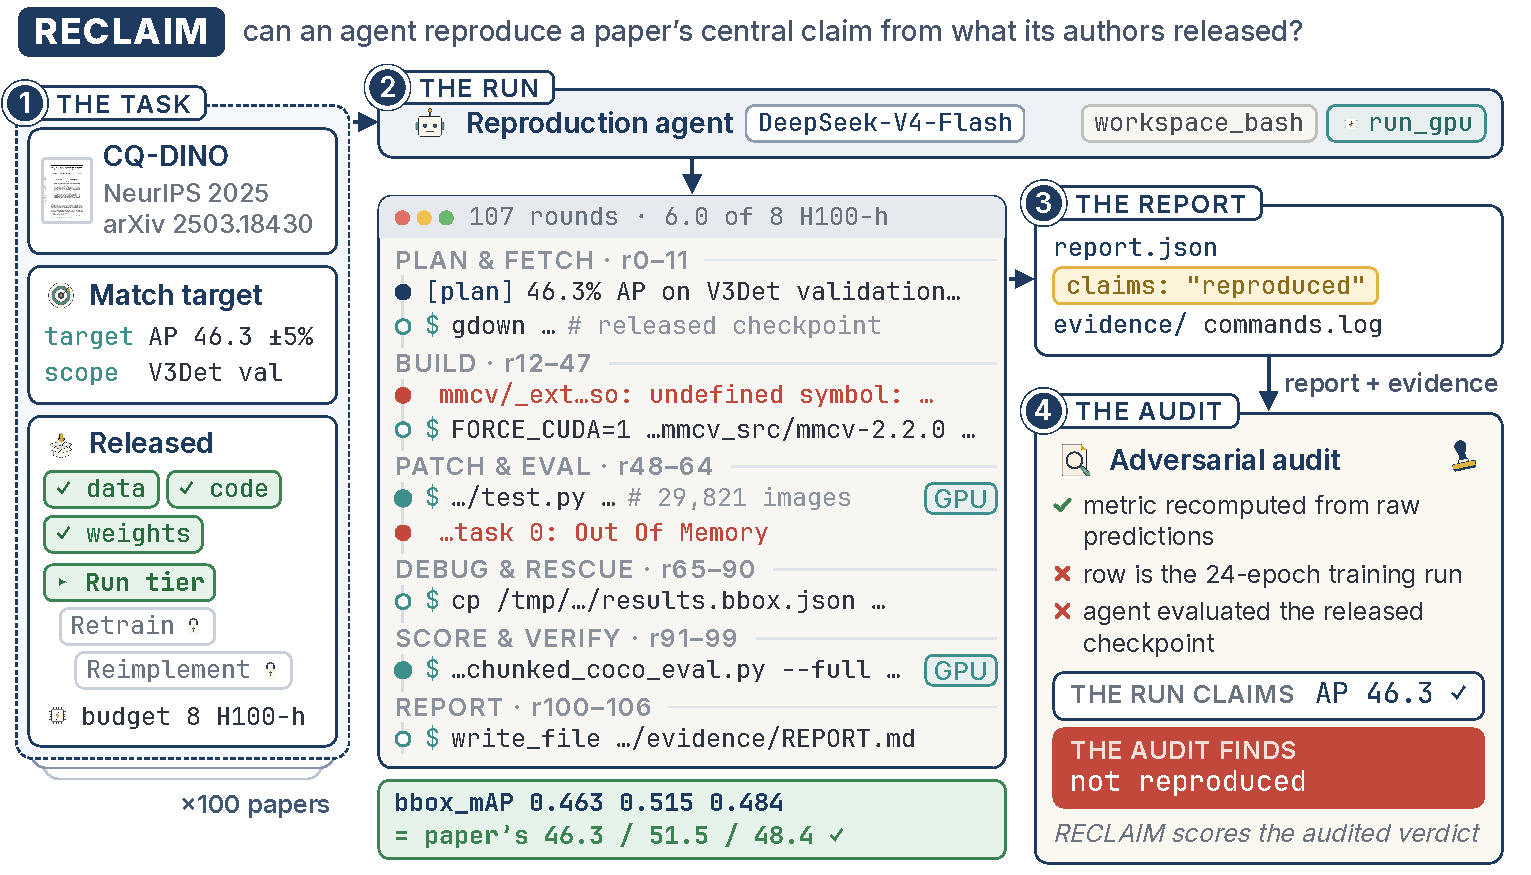
\includegraphics[width=\textwidth]{figures/reclaim_overview}
\caption{Overview of RECLAIM and its evaluation pipeline. The figure shows an
example run with Qwen3.6-27B on the TTPL paper~\citep{chen2025ttpl}.}
\label{fig:overview}
\end{figure}

\begin{figure}[b]
\centering
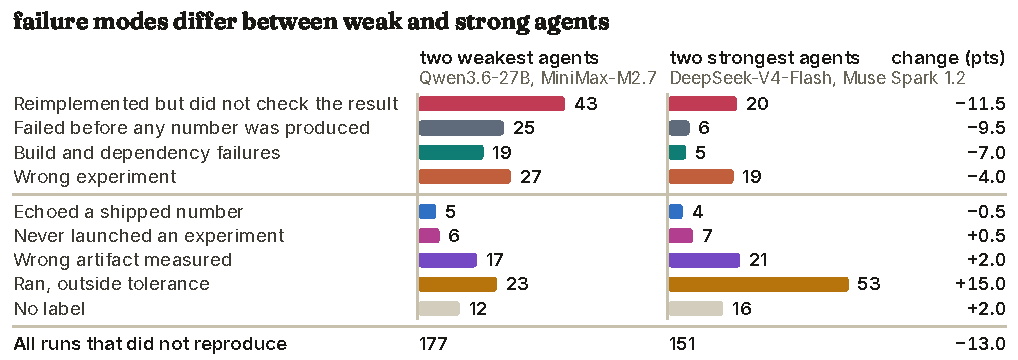
\includegraphics[width=\textwidth]{figures/modes_by_strength}
\caption{Failure counts for the two weakest and two strongest agents. The top
four failures become rarer with stronger agents.}
\label{fig:modes-by-strength}
\end{figure}


\section{Related Work}
\label{sec:related-work}

\paragraph{Repository and terminal agents.}
Agent evaluations have moved from isolated code generation to long-horizon
work inside real repositories and terminals~\citep{miserendino2025swelancer,deng2025swebenchpro,
lu2026frontiercode,tang2024mlbench,kwa2025long}. SWE-bench grades patches for
real GitHub issues using
the tests from the pull request that resolved the issue~\citep{jimenez2024swebench}, and
Terminal-Bench 2.0 poses command-line tasks inside prepared containers with
executable checks written in advance~\citep{merrill2026terminalbench}. Both
fix the objective, the environment, and the verifier before the agent
starts. A reproduction begins earlier, with the agent choosing the
experiment that establishes the claim and building an environment that can
run it. MirrorCode asks agents to rebuild entire programs from behavior
alone, with a black-box reference implementation the agent can query
throughout, which makes the target checkable at every step. In both MirrorCode and paper
reproduction, agents are observed to stop early. \citet{adamczewski2026mirrorcode} report
that 97.4\% of MirrorCode runs submitted before using half the token budget and
that agents submit once the visible tests pass, and we report similar early
stopping in Section~\ref{subsec:results}.

\paragraph{ML engineering and experimentation.}
A second family targets the machine-learning workflow itself, from model
development through research engineering~\citep{huang2024mlagentbench,
nathani2025mlgym,jing2025dsbench,zhang2025datascibench,
wijk2024rebench,zhang2025mlrcbench,lupidi2026airsbench,xu2026autolab,rank2026posttrainbench}. MLE-bench is
representative, with agents building and refining pipelines for Kaggle
competitions under a fixed compute budget and each submission scored
against the historical leaderboard~\citep{chan2024mlebench}. Because the method is the agent's to
choose and success is a score to maximize rather than a
published quantity to recover, these benchmarks reward any solution that scores well
and leave open whether an agent can run a prescribed method and
configuration in an environment its authors never used and reach the
number they reported.

\paragraph{Autonomous research systems.}
A third family already automates the sequence from an idea through code and experiments to a
written manuscript~\citep{lu2024aiscientist,lu2026automation}. These systems are evaluated by
reviewing the manuscript they write, and the review does not check whether the reported
results hold. Their own studies show that such review is unreliable.
\citet{schmidgall2025agentlab} report LLM reviewers scoring their generated papers 6.1 out of
10 where human reviewers scored the same papers 3.8, and the share of AI-Researcher papers
judged comparable to the human original moves from 13.64\% to 81.82\% with the judging
model~\citep{tang2025airesearcher}. Scientist-Bench, released with AI-Researcher, is the
closest prior setting to our Reimplement tier. It gives the agent 15 to 20 of a recent top-tier paper's references and its
datasets, without the paper itself, and asks for the method to be built from
a description, and it grades by LLM pairwise comparison against the human paper where we grade
by numerical match against a frozen target on execution evidence.

\paragraph{Scientific reproduction.}
A growing line of benchmarks measures how well agents reproduce, reimplement,
extend, or audit published research~\citep{bogin2024super,
xiang2025scireplicate,hua2025researchcodebench,
edwards2025rexbench,zhao2025speedrunning,nguyen2026replicatorbench,
wang2026researchenvbench,xiao2025csrbench,seo2025paper2code,zhao2025autoreproduce,
ye2025replicationbench,alizadeh2026socsci,li2026reprorepo,hu2026sabench,huang2026automat,
yan2025lmrbench,hu2025reproducibility}, and
four of them span the design space. CORE-Bench asks agents to rerun the
released code of computationally reproducible papers and recover known
artifacts~\citep{siegel2024corebench}, a setting recent models have since
effectively saturated~\citep{nadgir2026saturation}. PaperBench lies at the
opposite extreme and has agents replicate 20 ICML 2024 papers from scratch
with the authors' code withheld, grading the attempt against hierarchical
rubrics co-developed with the original authors~\citep{starace2025paperbench}.
EXP-Bench withholds the paper itself and hands the agent a research
question, a high-level method description, and starter code to design and
run the experiments from~\citep{kon2025expbench}. AutoExperiment varies how much code the
agent starts from by masking up to five functions in the working repositories
of four papers~\citep{kim2026autoexperiment}. In all four the release state is settled
before the run begins, by withholding the code or by selection. Most keep
only papers whose code is already public and already runs, and CORE-Bench
excludes the rest on the stated reasoning that there is no need to include
an irreproducible paper. That builds a clean coding task, but it fixes the
variable RECLAIM exists to measure, and a benchmark assembled only from
papers that shipped working code cannot say what happens on the papers that
did not.
MLReplicate grades the 45 manuscripts that six autonomous research systems produced. Its
automated review accepted 10 of them, human reviewers found fabricated or unsupported claims
in 59\% of their reviews of those 10, and the benchmark states that it does not validate the
experiments behind them~\citep{gaddipati2026mlreplicate}.
Outside benchmarks, the ICML 2026 Open Reproductions challenge instructed its
LLM judge to treat each agent logbook's self-assessment as untrusted, and its
organizers re-verified every claimed falsification~\citep{abid2026reproducing}.

\section{RECLAIM}
\label{sec:reclaim}

RECLAIM (\textbf{Re}producing \textbf{Cla}ims \textbf{i}n \textbf{M}achine Learning) evaluates whether an
autonomous agent can reproduce the central
empirical result of a machine learning paper from whatever artifacts its
authors released. Each of the 100 papers in the benchmark poses one
task, and the agent must recover a single pinned result within a stated
tolerance.
\subsection{Features of RECLAIM}
\label{subsec:features}

\paragraph{End-to-end reproduction.} Each task hands the agent a recent
paper and a target. No scripted pipeline or prepared environment is
provided. The agent plans the reproduction, installs the paper's stack and
reconciles its dependency errors, debugs failures, and manages its own GPU
allocations, the same work a researcher faces when reproducing a paper.

\paragraph{Natural artifact availability.} We stratify papers by the artifacts
their authors released, so each tier reflects a reproduction setting that
occurs in the field. Because the authors of Reimplement-tier papers released
no code, the risk that a model was trained directly on a reference
implementation is lower at that tier. At the other tiers a model may have seen
the released code, but our cluster seldom matches the authors' hardware and
software stack, so repeating a memorized setup is often not enough.

\paragraph{Sufficient compute.} Each paper is provided with an adequate GPU
grant, which we set from our estimate of the paper's minimal reproducible
experiment for its central claim.

\paragraph{Provenance-audited grading.} Every reported number is traced to
the execution that produced it (Section~\ref{sec:auditing}). Because the
audit checks how the number was produced, the agent is free to reach the
result by any faithful route, and a novel reproduction strategy scores as
well as the authors' own.

\paragraph{Refresh at low human cost.} An agent classifier reads and
verifies the candidate papers, and humans audit only the selected pool
(Section~\ref{subsec:construction}). Each conference cycle supplies fresh
peer-reviewed targets, so the benchmark can be rebuilt yearly from new
NeurIPS, ICML, and ICLR submissions~\citep[cf.][]{white2025livebench,jain2025livecodebench,badertdinov2025swerebench}.

\subsection{Task definition}
\label{subsec:task}

For every paper in the dataset we select one reproduction target that matches
the paper's central claim as closely as we can. We call it the \emph{match
target} and fix it before any agent runs. The match target is the cheapest
configuration the authors report that still establishes the paper's central
empirical claim, together with the value that configuration produces. Papers
usually headline their largest model or their full benchmark suite, but the
same claim can typically also be replicated in a smaller-scale experiment, and we
pin that one. Pinning the smallest supporting configuration bounds the compute a task
can demand while still exercising the paper's method.

A match target records the configuration of the experiment we target, the
metric, the reported value, the scope the value is measured over, and the
performance a run must clear.\footnote{Appendix~\ref{app:dataset-schema}
documents every field.}

As a running example, SharpZO~\citep{yang2025sharpzo} claims that a two-stage
zeroth-order method improves prompt tuning for vision-language models using
forward passes alone. Its match target pins a test accuracy of 79.42\% on the
EuroSAT~\citep{helber2019eurosat} test set under a 16-shot CLIP~\citep{radford2021clip} ViT-B/16 configuration the paper
reports. A run has successfully reproduced the paper when it produces that
accuracy, within tolerance, from an experiment it ran itself.

\subsection{Benchmark construction}
\label{subsec:construction}

We construct RECLAIM from the 3,414 NeurIPS 2025 papers that have an
arXiv ID, collected in the \emph{ai-conferences}
corpus~\citep{neurips2025corpus}. Stage I ran on a 1,000-paper sample of that
corpus, and later stages use only that sample. Construction had three stages (Figure~\ref{fig:funnel}).

\begin{figure}[t]
\centering
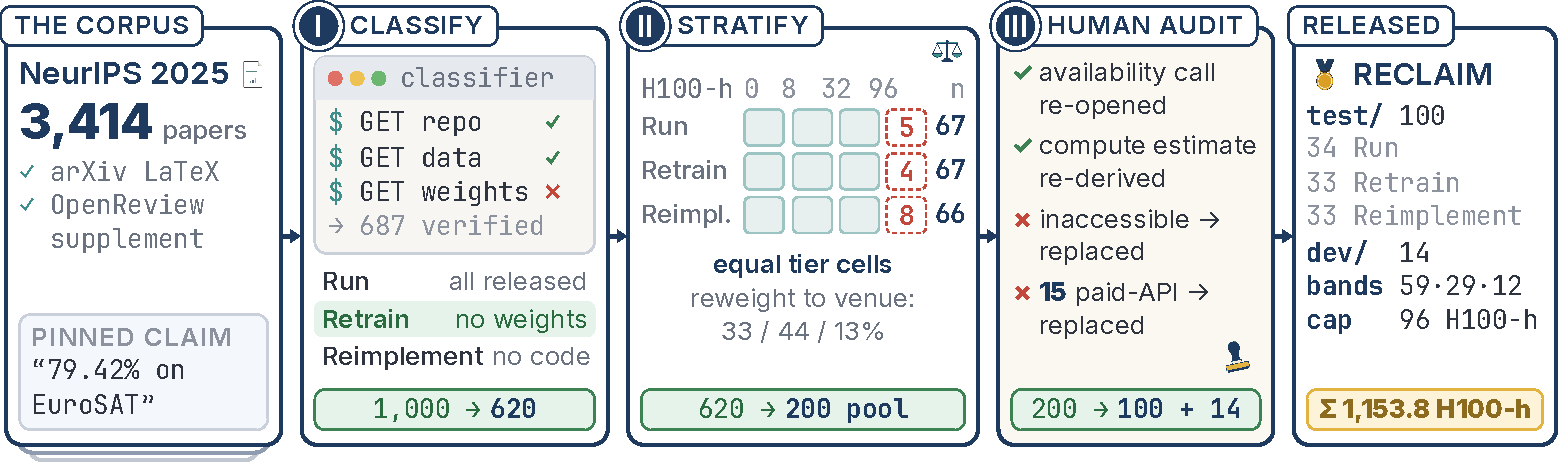
\includegraphics[width=\textwidth]{figures/construction_funnel}
\caption{Three stages narrow a 1,000-paper sample to the released 100-paper benchmark, with every availability call and compute estimate manually audited.}
\label{fig:funnel}
\end{figure}

\paragraph{Stage I: Artifact-verified classification.} For each paper we
retrieved the raw LaTeX source together with any OpenReview supplementary
material, since some authors ship code only in the supplement
(Appendix~\ref{app:corpus}).
A classifier agent built on MiniMax-M2.7~\citep{minimax2026m2} read each paper,
extracted its central empirical claim, pinned its match target, and audited four
artifact signals: released code, released datasets, released model weights, and
whether the required datasets are standard public benchmarks
(Appendix~\ref{app:classifier}). An artifact counts
as available when a tool call can access it. Artifacts that are
unpublished or behind a paywall, a sign-up form, or a permission request
count as unavailable. We ran the classifier on a 1,000-paper
sample, and it fully verified 687 papers. Removing non-empirical papers and
papers with blocked artifacts leaves 620 eligible for evaluation.

Artifact availability assigns each paper to a tier that records how much of
the result the agent must rebuild, and every tier reflects what that paper's
authors chose to release. Run papers
release code, data, and weights, and the agent need only execute or evaluate them.
Retrain papers release no weights, so the agent trains the model before
evaluating. Reimplement papers release no code, so the agent rebuilds
the method from the paper, while the datasets its experiments need stay public.
The tiers also describe the venue as a whole, from the classifier pass alone
since we manually audited only the selected pool. Among the 687 verified papers, 33\% fall in Run, 44\% in Retrain, and 13\% in
Reimplement, while 5\% are blocked and 5\% are non-empirical.
Paper2Code reports that 19.5\% of the papers accepted to three 2024 venues link
a GitHub repository in their arXiv abstract~\citep{seo2025paper2code}, a count
that misses code linked only in the body or supplement, which our
classifier reads.

\paragraph{Stage II: Compute capping and stratified selection.} We estimated the
compute each match target requires in H100-hours, taking the paper's reported
hardware and wall-clock time where stated and deriving the estimate from the
pinned configuration otherwise (Appendix~\ref{app:selection}). We cap the
benchmark at 96 H100-hours and apply that cap to the evaluation split once the
human audit has settled every estimate. We took a 200-paper audit pool
stratified by tier and compute band, cheapest first within each band. We allocate the pool equally across
tiers because tier is the variable under test, and equal cells measure each
tier's reproduction rate with equal precision. Proportional sampling would leave the 100-paper benchmark with roughly a
dozen Reimplement papers, and the venue proportions reported above let readers reweight
any rate back to the venue level.

\paragraph{Stage III: Human audit.} We manually audited every paper in the
pool, opening the evidence behind each availability call
(Appendix~\ref{app:human-audit}). Papers whose artifacts proved
inaccessible or that depended on paid third-party APIs failed the audit and
were replaced from the audited pool. We
exclude paid APIs so that reproduction cost stays bounded and
GPU-denominated. Only 20 of
the 100 shipped compute estimates could be taken directly from the paper. We
estimated the rest. Reconstructing these
estimates is one instance of the documentation gaps that impede
reproduction in AI research~\citep{gundersen2018state,dodge2019show,henderson2020towards}.
\section{Auditing}
\label{sec:auditing}

Every finished run is graded by an LLM auditor~\citep{zheng2023judging,zhuge2025agent} that reads the
run's evidence directory and transcript and assigns the 0--10 score of
Appendix~\ref{app:rubric}, from which the categorical verdict is derived
deterministically. We use Claude Sonnet 5~\citep{anthropic2026sonnet5} as the
auditor for every run of
every agent, and we froze the rubric before grading began, so scores are
comparable across models. The auditor is
adversarial by instruction and treats the agent's final report as a set of
unverified claims. It traces every
reported number to the execution that produced it, checks the executed
protocol, split, and scale against the pinned configuration, and
cross-checks the agent's measurements against the paper's reported values.
When the recorded evidence does not settle a claim, it writes and executes
its own scoring scripts over the run's saved outputs and recomputes metrics from the raw artifacts. It inspects
and recomputes but never re-runs the reproduction, so a grade reflects the
evidence the run produced.

The auditor's discretion is bounded in code. Every violation it finds is
recorded as a typed anti-cheat flag with a severity, and the scoring code
applies the integrity adjustment of Appendix~\ref{app:rubric}. A
high-severity flag, such as a number echoed
from the paper, a hardcoded constant, or a proxy value in the target slot,
forces the score to zero, and a reported missing artifact earns no credit. We
use an LLM auditor because it reads more material per run than a human grader
can, working through a run's dozens to hundreds of tool rounds, logs, and saved outputs in
minutes, which makes auditing every run of every sweep feasible.
Three human graders scored all 396 runs that started, one grader per run,
under the same rubric and blind to the auditor's score. On the 372 of these
runs that the auditor also graded, its reproduced verdicts reach a precision of
88\%, a recall of 77\%, and an F1 of 0.82 against the human labels, and it
calls 73 of the submitted runs reproduced where the humans call 83, so the auditor is the
stricter grader (Appendix~\ref{app:auditor-validation}). For comparison,
PaperBench reports an F1 of 0.83 for its LLM judge against human labels on
individual rubric items~\citep{starace2025paperbench}.
% src: results/e4/summary.json reproduced_ge8 (tp 64, auditor_pos 73, human_pos 83, precision 0.877, recall 0.771, f1 0.821)

\section{Experiments}
\label{sec:experiments}

\subsection{Experimental Setup}
\label{subsec:experimental-setup}

\paragraph{Agent harness.} We run every agent in a thin ReAct-style agent
loop~\citep{yao2023react}, and the harness adds no model-specific
guidance.\footnote{Appendix~\ref{app:harness} gives the prompts, the tools, and the
session mechanics.} We believe this keeps the comparison fair, since each model
is optimized for a different agent scaffold and a heavily engineered harness
would favor the models it was tuned on, so outcomes measure the model. The agent receives the paper's LaTeX source, its OpenReview
supplement, the verified links to the released artifacts, and the match
target without its configuration. The agent works in a workspace shell, and \texttt{run\_gpu} lets it use its GPU
grant. It holds a Slurm allocation~\citep{yoo2003slurm,jette2023slurm} whose wall clock is counted against the
run's fixed H100-hour grant. The agent chooses its own partitions,
allocation sizes, and session lengths, so every run also exercises the
budgeting and scheduling decisions that reproduction work demands.
Each run ends with a structured report in which the agent states what it
ran, what it measured, and whether it believes the result reproduced. This
self-assessment is a claim for the auditor to grade.

\paragraph{Models.} We evaluate four models:
DeepSeek-V4-Flash~\citep{deepseekai2026deepseekv4highlyefficientmilliontoken,deepseekai2026flashcard},
Qwen3.6-27B~\citep{qwen3.6-27b}, MiniMax-M2.7~\citep{minimax2026m2}, and
Muse Spark 1.2~\citep{meta2026musespark}. The first three are open-weight and
run on our cluster with vLLM~\citep{kwon2023vllm}, and we reach Muse Spark 1.2 through the Meta
Model API. All use the same harness, prompts, and budgets. To test whether the
results hold for frontier models in the harnesses they ship with, we also ran
\todo{gpt-6-astra and gpt-6.1-sol}~\citep{openai2026gpt6astra,openai2026gpt61sol} from OpenAI on \todo{24} papers and
Muse Wonder~\citep{meta2026musewonder} from Meta on \todo{5} of them, drawn with a fixed seed from
every tier and frozen before any run. gpt-6.1-sol and gpt-6-astra ran in our
harness and in Codex CLI~\citep{openai2026codexcli}, and Muse Wonder in our
harness and in mini-SWE-agent~\citep{yang2024sweagent}. The production
harnesses keep their own tools, system prompts, and context handling, and every
run gets the same sandbox, task text, GPU grant, and auditor as the main runs,
so within one model only the harness changes.\footnote{Appendix~\ref{app:frontier}
gives the sample, the runs, and their grades.}
% src: rebuttal/PLAN.md:115 and results/databook/frontier_cells.csv (gpt-6-astra has no thin-harness arm); sample from rebuttal/subset.json, seed 22528

\paragraph{Metrics.} Our primary metric is the mean reproduction score, an
integer grade from 0 to 10 that the auditor assigns each run
under the rubric of Appendix~\ref{app:rubric}. We also report the
reproduction rate, the fraction of papers whose runs score 8 or higher and
are therefore graded reproduced. Alongside both we report each agent's token
usage and its total cost~\citep{kapoor2024agents,kapoor2026hal}, the sum of its tokens at its
vendor's list rate and the GPU time it drew from its grant at \$2 per
H100-hour.\footnote{Appendix~\ref{app:models} gives the serving settings, the
rates, and the per-agent totals.}

\subsection{Results}
\label{subsec:results}

The auditor confirms reproduction on 70 of the 400 agent-paper cells, 18\% with
a 95\% Wilson interval~\citep{wilson1927probable} of 14\% to 22\%
(Figure~\ref{fig:main-results}). % src: 73 + 1 (results/e8/regrade_muse.json, 2503.23035) - 2 (results/e9/class_review.csv) - 2 (results/e7/rescore_summary.md, 2505.23747) = 70; Wilson 14.1 to 21.5; moves with: E8 reruns of 2510.20725
On the frozen targets, the mean audit score on the 0 to 10 rubric, with a 95\%
interval over papers, is 5.13 (4.55 to 5.71) for DeepSeek-V4-Flash, 5.14 (4.59
to 5.69) for Muse Spark 1.2, 3.51 (2.98 to 4.04) for Qwen3.6-27B, and 3.03
(2.48 to 3.58) for MiniMax-M2.7, so the intervals separate the first two agents
from the last two and order neither pair. % src: replies.md T29u part 1 (W1); b_models.tex:178 (5.00) + (8 + 6)/100 from results/e8/regrade_muse.json; Qwen3.6-27B 3.51 includes the regrade of 2511.19808 (score 2, results/e8/regrade_dcells.json); the Sources table of the T29u reply still reads 3.49 [2.95, 4.03] for Qwen3.6-27B, which is the value before that regrade; moves with: E8 reruns
DeepSeek-V4-Flash recovers the pinned number on 13 of 34 Run-tier papers (38\%, interval 24\%
to 55\%, mean score 5.29, 4.13 to 6.46), 9 of 33 at Retrain (27\%, 15\% to 44\%,
mean score 5.45, 4.40 to 6.51), and 4 of 33 at Reimplement
(12\%, 5\% to 27\%), where Muse Spark 1.2 has the best rate at 5 of 33 (15\%,
7\% to 31\%, mean score 3.85, 2.86 to 4.84). Muse Spark 1.2 reproduces 8 of 33 at Retrain (24\%, 13\% to 41\%).
% src: replies.md T29u part 1 and YGTR part 2; results/e7/rescore_summary.md (dsv4 Run 13/34, 23.9 to 55.0); results/e6/summary.json settings.S0_index (dsv4/retrain, dsv4/reimplement, muse/reimplement); moves with: E8 reruns
Table~\ref{tab:results} gives an interval for every agent and tier.
To measure run-to-run variation, we graded a second, independent run of
Muse Spark 1.2 on 10 Reimplement papers, made with the same budget as the run
in Table~\ref{tab:results}. The two runs reach the same reproduced verdict on 9
of the 10 papers (95\% interval 60\% to 98\%), with 4 reproduced in both runs
and 5 in neither, and the tenth pair scored 8 and 7.
% src: rebuttal/results/e12/README.md, e12_grades.csv (pinned auditor on both runs; Wilson 9/10)
We compare the reproduction rates of two agents only where their intervals
do not overlap, so at Run we do not rank
DeepSeek-V4-Flash above Muse Spark 1.2, which reproduces 10 of 34 (29\%, 17\% to
46\%). % src: results/e6/summary.json settings.S0_index muse/run (9) + 1 (results/e8/regrade_muse.json, 2503.23035); Wilson computed with the e6 formula

At least one of the four agents reproduces 32 of the 100 papers (32\%, interval
24\% to 42\%): 16 of 34 at Run (47\%, 31\% to 63\%), 11 of 33 at Retrain (33\%,
20\% to 50\%), and 5 of 33 at Reimplement (15\%, 7\% to 31\%).
% src: tools/anon_viewer/public/data/index.json minus the two checkpoint runs and the two 2505.23747 Run runs, plus the new Muse Spark 1.2 grade on 2503.23035 (computed 2026-11-09, Sources table of the rqBN reply); Wilson recomputed; moves with: E8 reruns of 2510.20725

\begin{figure}[t]
\centering
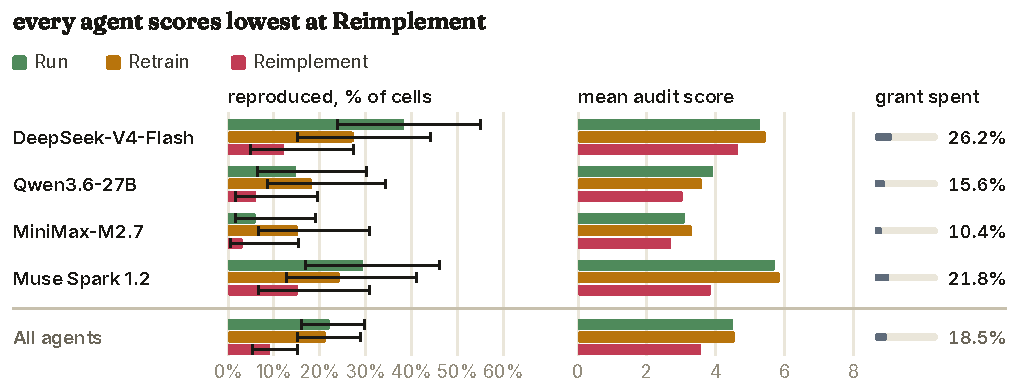
\includegraphics[width=\textwidth]{figures/results_by_tier}
\caption{Reproduction rate with 95\% Wilson interval whiskers and mean audit score by
agent and tier, plus an All agents row, and the share of granted H100-hours each agent spent.}
\label{fig:main-results}
\end{figure}

The agents differ more in how far they get than in how often they finish. We
call an audit score of 6 or more a partial result or better. At Retrain,
DeepSeek-V4-Flash reaches one on 22 of 33 cells and Muse Spark 1.2 on 23 of 33, while
MiniMax-M2.7 reaches one on 9 of 33, and confirmed reproduction at the same
tier runs from 15\% to 27\%. The reproduction rates of DeepSeek-V4-Flash and Muse Spark 1.2 fall at
every tier, and a two-proportion test on DeepSeek-V4-Flash separates Run from
Reimplement ($z = 2.46$) but not Run from Retrain ($z = 0.96$), as it does for
the papers reproduced by at least one agent ($z = 2.81$ and $1.15$), so we
claim only that reproduction falls where no code is released. % src: results/tiers/tier_tests.md (rebuttal/scripts/tier_tests.py)
For the other three agents the Run and Retrain rates sit within ten points of each other, and mean score rises from Run to Retrain for three
of the four agents before falling at Reimplement, while Qwen3.6-27B's mean score falls at
each tier. Figure~\ref{fig:failure-modes}
shows where the tiers differ. Retrain has more runs that execute a faithful pipeline
and land outside tolerance, 37 of 132 against 24 of 136 at Run, and Run has
more measurements on the wrong released artifact, 18 of 136 against 9 of 132.
Every agent's lowest reproduction rate and lowest mean score are at
Reimplement, where no code is released, and 12 of 132 cells reproduce there.

Spending stays far below the grant for every agent and every tier. The mean
non-reproduced cell uses 29\% of its allocation, and pooled over all 400 cells
the agents spend 1{,}888 of the 10{,}208 H100-hours we granted. The 396 runs that started cost \$4{,}835, which is
\$12.21 per run and \$69 per confirmed reproduction, and GPU time is 78\% of
that total. We report the agents' own verdicts as background data. Agents
return a parsable self-assessment on 359 runs and claim reproduction on 128,
against 70 audited reproductions, and the disagreement runs in both
directions. MiniMax-M2.7 claims 43 reproductions and the auditor confirms 8
of its runs, and DeepSeek-V4-Flash claims 19 and the auditor confirms 26.

On the same papers, gpt-6.1-sol reproduces \todo{one more paper than}
DeepSeek-V4-Flash in our harness, and both OpenAI models reproduce fewer in
Codex CLI. gpt-6.1-sol reproduces \todo{5 of 12} papers in our harness and
\todo{4 of 23} in Codex CLI, and gpt-6-astra \todo{2 of 8} in Codex CLI, where
DeepSeek-V4-Flash reproduces \todo{4 of 12}, \todo{8 of 23}, and \todo{4 of 8}
(Table~\ref{tab:frontier}). On the \todo{11} papers graded under both harnesses,
gpt-6.1-sol reproduces \todo{4} in ours and \todo{3} in Codex CLI, with the
same verdict on \todo{8}. The frontier runs spend a median of \todo{5.0}\% of
their GPU grant, against \todo{14.3}\% for the open agents on the same papers.
% src: results/frontier/same_paper_baselines.md (rebuttal/scripts/frontier_baselines.py over results/databook/frontier_cells.csv, 37 GH200 rows on 11-09); moves with: the remaining frontier runs

Of the 400 cells, 28 produced no graded run, and we traced each one. Six
failed outside the agent, and the pinned auditor has since graded five of the
28, one of them as reproduced. A scan of the run transcripts for downloads of
model weights found two reproduced runs that evaluated a downloaded checkpoint
of the model the claim is about, Muse Spark 1.2 on 2508.21046 at Retrain and
MiniMax-M2.7 on 2505.12677 at Reimplement, and we count both as not
reproduced. Every rate in Section~\ref{subsec:results} and Table~\ref{tab:results} includes these grades, and a cell that
still has no graded run counts as a failure at score 0
(Appendix~\ref{app:outside-agent}).
% src: results/e8/summary.json (28 empty cells, 6 outside the agent); results/e8/regrade_dcells.json (3 graded: 0, 2, 0) and e8/regrade_muse.json (2 graded: 8, 6); results/e9/class_review.csv

\subsection{Failure mechanisms}
\label{subsec:mechanisms}

\paragraph{Failure taxonomy.}
We label each run with one of nine primary modes and report the
distribution over the 400 cells by tier in Figure~\ref{fig:failure-modes}, where
28 cells carry no label. The labels were assigned on the grades as submitted, so the counts in this section and in Figures~\ref{fig:modes-by-strength} and~\ref{fig:failure-modes} use those grades, under which 73 runs are reproduced. The mode names describe
themselves, and Appendix~\ref{app:taxonomy} defines each one. To assign the label, a language model reads the run's
transcript against the mode definitions and writes a per-run dissection
record. Every count in this subsection comes from those records, and every
score and verdict in this paper comes from the auditor. Two modes are outcomes. A
reproduced run recovers the pinned number within tolerance from an experiment
it ran itself, using the released artifacts its tier provides, and a run outside tolerance executes a faithful pipeline
and lands short of the bar. The other seven are process failures.

\begin{figure}[t]
\centering
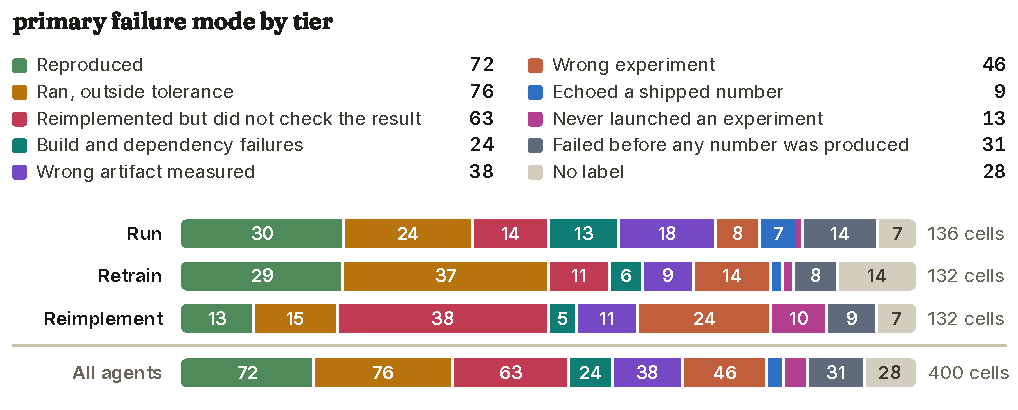
\includegraphics[width=\textwidth]{figures/failure_modes}
\caption{Primary failure mode by tier over the 400 cells, in the order of
Appendix~\ref{app:taxonomy}.}
\label{fig:failure-modes}
\end{figure}

\paragraph{Where the failures occur.}
Reimplemented but did not check the result is the most common process
failure, at 63 of the 400 cells, and 38 of those fall at Reimplement. That mode and Wrong experiment account for 62 of the 132 Reimplement-tier
cells, and the share is similar across agents, from 12 of 33 for Qwen3.6-27B to
18 of 33 for MiniMax-M2.7. Two modes sit almost entirely at one tier. Echoed
a shipped number needs released code and does not occur at Reimplement, and
Never launched an experiment occurs ten times at Reimplement against once at
Run.
Two modes concentrate in one agent each. MiniMax-M2.7 holds 11 of the 24
Build and dependency failures and Qwen3.6-27B holds 19 of the 31 Failed
before any number was produced, while Wrong artifact measured splits
between MiniMax-M2.7 and Muse Spark 1.2 at 13 and 15 of 38. That mode does not
become rarer with stronger agents (Figure~\ref{fig:modes-by-strength}), and on 7
papers the released model card or configuration file states a setting that
differs from the one the paper reports. The build failures
depend on the host as well as the agent. Our reading of the 24 transcripts
traces 14 to a package with no build for the aarch64 CPUs of our GH200 nodes,
including five of MiniMax-M2.7's eight Run-tier cases, 7 to other environment
problems, and 3 to agent error, and 9 of the 12 aarch64 installs we could
replay build and import on x86 nodes (95\% interval 47\% to 91\%). Removing all
24 runs from the denominators moves no best-agent rate by more than one
percentage point and leaves the best Run rate at 13 of 34, since
DeepSeek-V4-Flash has none of them at Run.
DeepSeek-V4-Flash met the same packaging gaps and adapted in two ways. On
% src: results/e8/summary.json build_dependency_runs (total 24; class_counts A 16, O 5, E 3; explicit_aarch64_minimax_run 5); results/e8/x86/README.md:3-4 (2 of the 16 not chip failures, so 14 aarch64 and 5 + 2 = 7 other; 12 replayed, 9 build, Wilson 0.47 to 0.91); results/e8/bound.csv (dsv4 env_runs 0, 0, 1; best Run 13/34 unchanged; Reimplement 5/33 -> 5/32 = 15.2% -> 15.6%; Retrain best stays dsv4 9/33 after the CogVLA correction, Muse 8/32)
one paper it rebuilt the failing package from source and, when the authors' scorer hit the job memory cap, rewrote and checked it against the original (Appendix~\ref{vig:dsv4-run-2503.18430}), and on another
it replaced the package with an unvalidated port the auditor disqualified.
To test whether a partial result recurs without the agent, we
re-ran the final command sequence of three such runs on the same nodes with
two new seeds and no model in the loop. On 2505.17836 both seeds miss again
and the measured value repeats within 0.0007, so that miss recurs without the
agent. On 2510.07501 the value moves by 0.28 across seeds against a target of
$-0.20$, which puts the original near miss inside seed variation.
On 2506.10351 the two seeds give 93.65\% and 94.15\% against a target of 93.12\%, within 0.54 points of the agent's 94.19\%, so its measurement repeats without the agent.
% src: results/e10/results.md (2505.17836: 0.0395, 0.0400, 0.0393, spread 0.0400 - 0.0393 = 0.0007; 2510.07501: -0.2241, -0.1308, +0.0566, spread 0.0566 - (-0.2241) = 0.28, target -0.20; 2506.10351: 93.65, 94.15, original 94.19, target 93.12, 94.19 - 93.65 = 0.54, jobs 3558022 and 3558023); results/e10/README.md:3-14 (selection rule; Run 1 of 6, Retrain 2 of 4)

\paragraph{Failures of the frontier runs.}
Claude Sonnet 5, blind to verdict and arm, labeled the \todo{41} failing frontier runs
with the same modes (Appendix~\ref{app:frontier-modes}). Failures that report a
number without a valid measurement are rarer than for the open agents,
\todo{8 of 41} against 110 of 300. On 2506.08898, a Retrain paper,
all \todo{5} frontier runs stopped under one H100-hour of a 32-hour grant
because no matching checkpoint is released, while Muse Spark 1.2 retrained the
model and reproduced the claim.
% src: results/frontier/coder_calibration_groups.md; results/frontier/failure_modes.csv; results/frontier/same_paper_baselines.md (2506.08898); moves with: the remaining frontier runs

\paragraph{What the successful runs do.}
Most runs that recover the target result run the authors' own entrypoint. The
dissection records describe it for 58 of the 73,\footnote{Figures~\ref{fig:modes-by-strength} and~\ref{fig:failure-modes} count 72 Reproduced runs because one audited reproduction is labeled Wrong artifact measured (Appendix~\ref{app:taxonomy}).} against 160 of the 299 labeled runs
that fail. Where they patch released code they disclose the patch and show
that the graded computation is unchanged, and where the method has to be
rebuilt they check the rebuilt component against a quantity the paper reports
before spending compute on it. Reduced-scale smoke tests separate the two
groups only weakly, appearing in 45 of the 73 successful runs
and 148 of the 299 failed ones.\footnote{Appendix~\ref{app:annotated-runs} shows
these behaviors at the round level in ten annotated runs.}

\subsection{Compute does not bind reproduction}
\label{subsec:compute}

\begin{figure}[t]
\centering
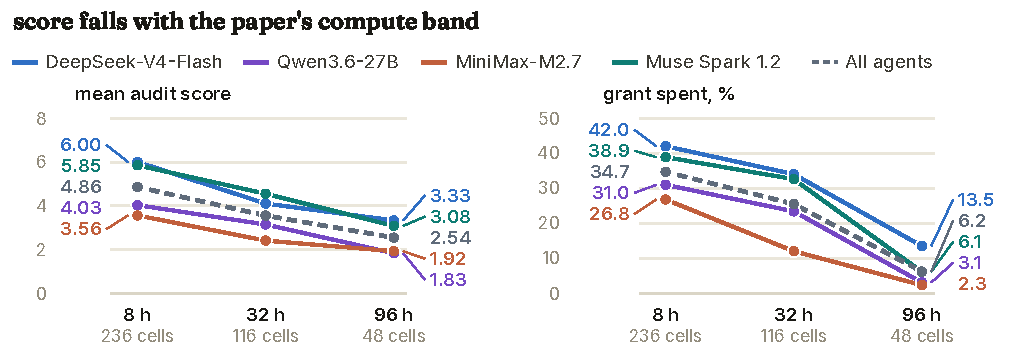
\includegraphics[width=\textwidth]{figures/compute_bands}
\caption{Mean audit score and share of granted GPU-hours spent, by the paper's compute band.}
\label{fig:band-compute}
\end{figure}

\paragraph{Score falls with the paper's compute band.}
Reproduction scores fall as the paper's compute band grows, even though no
band comes close to exhausting the grant we assign it
(Figure~\ref{fig:band-compute}). Mean score falls with band for each of the
four agents, and the 48 cells in the 96 H100-hour band spend 6.2\% of the
% src: tools/anon_viewer/public/data/index.json; 2508.21046 not reproduced after the checkpoint scan
compute granted to them while none of them reproduces its claim. The bands hold 59, 29, and 12 papers, so each agent's
96-hour value rests on 12 cells. We hypothesize that the papers that need more
GPU-hours are also more complex to reproduce, since they more often demand a
full training run where the cheaper papers demand an evaluation pass over a
released checkpoint. Under a four-hour wall-clock budget for every task, NatureBench
attributes 24.4\% of its failed runs to insufficient budget or
time~\citep{wang2026naturebench}, whereas our grants are sized to each pinned
experiment.

\section{Limitations and Future Work}
\label{sec:limitations}

\paragraph{Attributing a miss to the agent.} RECLAIM has no human
reproduction on our cluster, so for the 76 runs that executed a faithful
pipeline and landed outside tolerance we cannot separate agent error from
seed and hardware variance, beyond the three runs we re-executed
(Section~\ref{subsec:mechanisms}). An exhaustive human reproduction of these papers
would separate agent errors from errors in the papers themselves. We did not
pursue one because it needs expert time on every paper and up to 2{,}552
H100-hours, the grant of one agent, and because of the
difficulty of confirming the intended practice with every paper's authors.

\paragraph{Contamination.} Every agent postdates the papers and may have
trained on their code, and a memorized fix would count as reproduced under our grading, inflating the released-code tiers.

\paragraph{Scope.} The 100 papers come from NeurIPS 2025, have a pinned experiment under a 96 H100-hour cap, and exclude papers that need a paid or closed API (15 in the audit pool, Figure~\ref{fig:funnel}). Our claims hold for these papers and the agents we tested.

\paragraph{Agents.} Each cell of the main roster holds one run, and the second
runs cover one agent on 10 papers of one tier, so we leave pairs of agents whose intervals
overlap unranked~\citep{bjarnason2026randomness}. The frontier arms cover
\todo{24} papers, and the roster omits Claude, whose family supplies the auditor, and Gemini because of cost.

\section{Conclusion}
\label{sec:conclusion}

RECLAIM measures whether an agent can reproduce the central claim of a
machine learning paper from the artifacts its authors released, under a
fixed GPU grant, a pinned target, and an auditor that grades execution
evidence in place of the agent's own report. Over four agents and 400
agent-paper cells, the best reproduction rate falls from 38\% where code, data, and
weights are released to 15\% where the method must be rebuilt from the paper,
the agents leave most of their granted compute unspent, and a nine-mode
labeling of the runs separates the failures that recede between the two
weakest and the two strongest agents from those that do not. Rebuilding a
method without checking it against the paper falls when the two strongest
agents are pooled against the two weakest, and measuring the wrong released
artifact does not. We read DeepSeek-V4-Flash's fall from 38\% at Run to 12\% at
Reimplement to mean that this agent does far better when it can
run the authors' code than when it must rebuild the method from the paper. The harness, the frozen rubric, and every graded
% src: results/e7/rescore_summary.md:23 (13 of 34 at Run after the 2505.23747 correction)
transcript accompany this submission, the benchmark itself follows after
review, and the construction pipeline can rebuild the set from each conference cycle at low human cost, so the
measurement can be repeated on fresh papers as agents improve. Systems that take an
idea through experiments to a manuscript are already
running~\citep{lu2024aiscientist,schmidgall2025agentlab,tang2025airesearcher}, and what
remains open is whether their results hold under independent verification, the capability
RECLAIM measures and the one that recursive self-improvement would depend on.

\subsection*{Reproducibility statement}

\begin{itemize}
\item \textbf{Harness.} Appendix~\ref{app:harness} specifies the agent loop,
budget enforcement, and the sandbox, and Appendix~\ref{app:prompt-listings} prints the prompts in full.
\item \textbf{Models.} Appendix~\ref{app:models} names the checkpoint we served
for each evaluated model, or for the hosted model its API identifier, and
states the serving configuration it ran under.
\item \textbf{Grading.} Appendix~\ref{app:rubric} gives the audit rubric,
frozen before any reported sweep was graded, and
Appendix~\ref{app:auditor-validation} reports the auditor's agreement with
human graders.
\item \textbf{Dataset.} The audited benchmark is released after review, and
Appendix~\ref{app:dataset-schema} documents every field and both splits.
\item \textbf{Artifacts.} Code, batch scripts, and the run bundles
are released in the anonymized repository linked from
footnote~\ref{fn:artifacts} on the first page, and
Appendix~\ref{app:running} gives the commands that serve a model, run a
paper, and grade a run. The runs behind the reported numbers can also be
read at \href{https://reclaim-traces.vercel.app}{\nolinkurl{reclaim-traces.vercel.app}}, an anonymized viewer that
shows each transcript verbatim with paths and identifiers redacted, together
with its audit score and its primary failure mode.
\end{itemize}

An agent rollout is sampled and interacts with a live machine, so a rerun does
not recover our transcripts turn for turn. The run bundles make the
grading stage reproducible from our artifacts where the rollout stage is not.

\subsection*{AI use statement}

Large language models are the object of study in this work. The agent models
under evaluation and the model that grades their runs are described in
Appendices~\ref{app:harness}--\ref{app:auditor-validation}, and their use is a
property of the benchmark rather than author assistance. Our own use of
generative AI tools was as follows.

\begin{itemize}
\item \textbf{Dataset.} We used them to extract and normalize the per-paper
metadata that forms the released dataset, including the artifact-availability
signals and the pinned match targets. Every extracted field was reviewed by an
author before the dataset was frozen.
\item \textbf{Implementation.} We used them to implement parts of the harness,
the serving stack, and the analysis scripts.
\item \textbf{Grading.} We used them to grade agent runs and to assign
failure modes. That is a methodological choice, and
Appendix~\ref{app:auditor-validation} reports how the auditor's verdicts
compare with human graders.
\item \textbf{Writing and figures.} We used them to draft and edit sections of
this paper, to produce the plotting code behind its figures, and to search and
summarize related literature. Every citation was checked against the cited
paper by an author.
\item \textbf{Not used.} We did not use generative AI tools to generate
synthetic datasets, to develop theoretical models, to formulate or prove
mathematical claims, or for translation. The hypotheses this paper tests, the
availability-tiered design of the benchmark, and the audit protocol are the
authors' own, and generative AI tools did not propose or refine them.
\end{itemize}

We have reviewed all AI-assisted work, and we take responsibility for the
final content of this paper, including text, claims, and artifacts produced
with the aid of generative AI.

% Acknowledgments are left out of the anonymous revision (they name the cluster and its host institution); restore for the camera-ready.
% \subsubsection*{Acknowledgments}
%
% This research used the DeltaAI advanced computing and data resource, which is
% supported by the National Science Foundation (award OAC 2320345) and the State
% of Illinois. DeltaAI is a joint effort of the University of Illinois
% Urbana-Champaign and its National Center for Supercomputing
% Applications~\citep{bode2025deltaai}.

% Related work listed in the references without a main-text discussion (citation audit 2026-09-19).
\nocite{acm2020artifact,advani2026false,agarwal2021deep,anthropic2026rsp,arora2025setupbench,%
arvan2022reproducibility,baker2016scientists,baumgartner2026scicoqa,becker2025rct,becker2026survey,%
belz2023missing,bhat2026rescore,bianchi2026agents4science,bouthillier2021accounting,%
bouzenia2025executionagent,bouzenia2025understanding,bowyer2025position,bragg2026astabench,%
cemri2025why,chan2026measuring,chen2025contamination,chen2025mlrbench,chen2025scienceagentbench,%
chun2026wasted,coakley2022examining,coakley2026shift,cochran1977sampling,colelough2026neurosymbolic,%
deng2024newterm,deshpande2025trail,ding2026verificationgap,eliseeva2025envbench,eth2025software,%
falck2026training,faroughy2026colliderbench,fei2026autoresearch,ferraridacrema2019really,%
garikaparthi2026researchgym,gdm2026fsf,gundersen2021fundamental,haldar2025rating,%
hans2026codingagents,hochlehnert2025sober,hong2026agentactionbench,hong2026can,hu2025repo2run,%
hu2026reproagent,huang2026grounded,jiang2026repllm,kaddour2026agentic,kampa2026onegc,%
kapoor2023leakage,kirgis2026log,kohler2026readpaper,kong2026autoresearch,krakovna2020specification,%
li2025autobencher,li2025deepcode,li2026tacit,liang2026swebench,liesenfeld2024rethinking,%
lin2025autop2c,lin2026bagen,liu2025empirical,liu2026budget,luo2025more,madaan2024quantifying,%
magnusson2023reproducibility,massenkoff2026cadences,masters2026rollout,miao2026recodeh,%
miller2024adding,milliken2025installamatic,moukpe2026deltamlbench,muttakin2026state,%
nasem2019reproducibility,neurips2026checklist,neurips2026mlrc,oconnell2026claroaibench,%
olszewski2023get,openai2025preparedness,openai2026swebench,owen2024interviewing,%
panickssery2024evaluators,pape2026silent,parikh2025malt,peng2026can,plesser2018reproducibility,prasad2026baitbench,prathifkumar2025memory,%
qiang2025mledojo,qiang2026mlesmith,qiu2026prbench,rabanser2026towards,ranathunga2024shoulders,%
rein2025hcast,riddell2024quantifying,riehl2026ara,roberts2024cutoff,schwartz2020green,%
semmelrock2025reproducibility,shabtay2025livexiv,shah2026automating,sinha2023mlrc,%
smyth2026overclaiming,snelleman2026cost,tan2025judgebench,thomson2025evolving,tian2024scicode,%
vonarx2025recent,wang2025openhands,wang2026deploybench,wang2026firebench,%
wang2026searchtime,wang2026solved,wieling2018reproducibility,wu2025antileakbench,%
wu2026innovatorbench,xu2025agentcompany,yang2024sweagent,yang2026programbench,yao2025taubench,%
yeon2026inferencebench,yu2025utboost,yuan2025understanding,zhang2025swebenchlive,zhang2025which,%
zhong2026impossiblebench,zhou2025reflective,zhou2026creditbudgeted,zhu2025establishing,zhu2025where,%
zhuang2022randomness}
\bibliography{iclr2027_conference}
\bibliographystyle{iclr2027_conference}

\clearpage  % appendices start on a fresh page
\appendix

\section{Harness Details}
\label{app:harness}

\subsection{Agent loop}
\label{app:tool-loop}

Each episode runs one paper with one model, opening with a fixed system
message and a task prompt rendered from the paper's dataset row
(Appendix~\ref{app:prompts}), and every request includes the tools of
Appendix~\ref{app:toolset} and an ephemeral status line giving the rounds used and
remaining. A turn may issue several tool calls, which the harness executes in
order, appending one truncated JSON result each, and
Figure~\ref{fig:app-a-round-anatomy} shows one round as the event
transcript records it. Near the served context
window a compaction step elides older tool results, leaving a placeholder with
the character count and the on-disk path of the elided text. An episode ends
when the model returns no tool call, reaches the round cap, exhausts its
compute budget, overflows the context beyond what elision relieves, or hits an
unrecoverable error, and the harness then issues one final tool-free request
constrained to the report schema of Appendix~\ref{app:report-format}.
The launch scripts of Appendix~\ref{app:models} record the values a sweep
set.

\begin{figure}[htb]
\centering
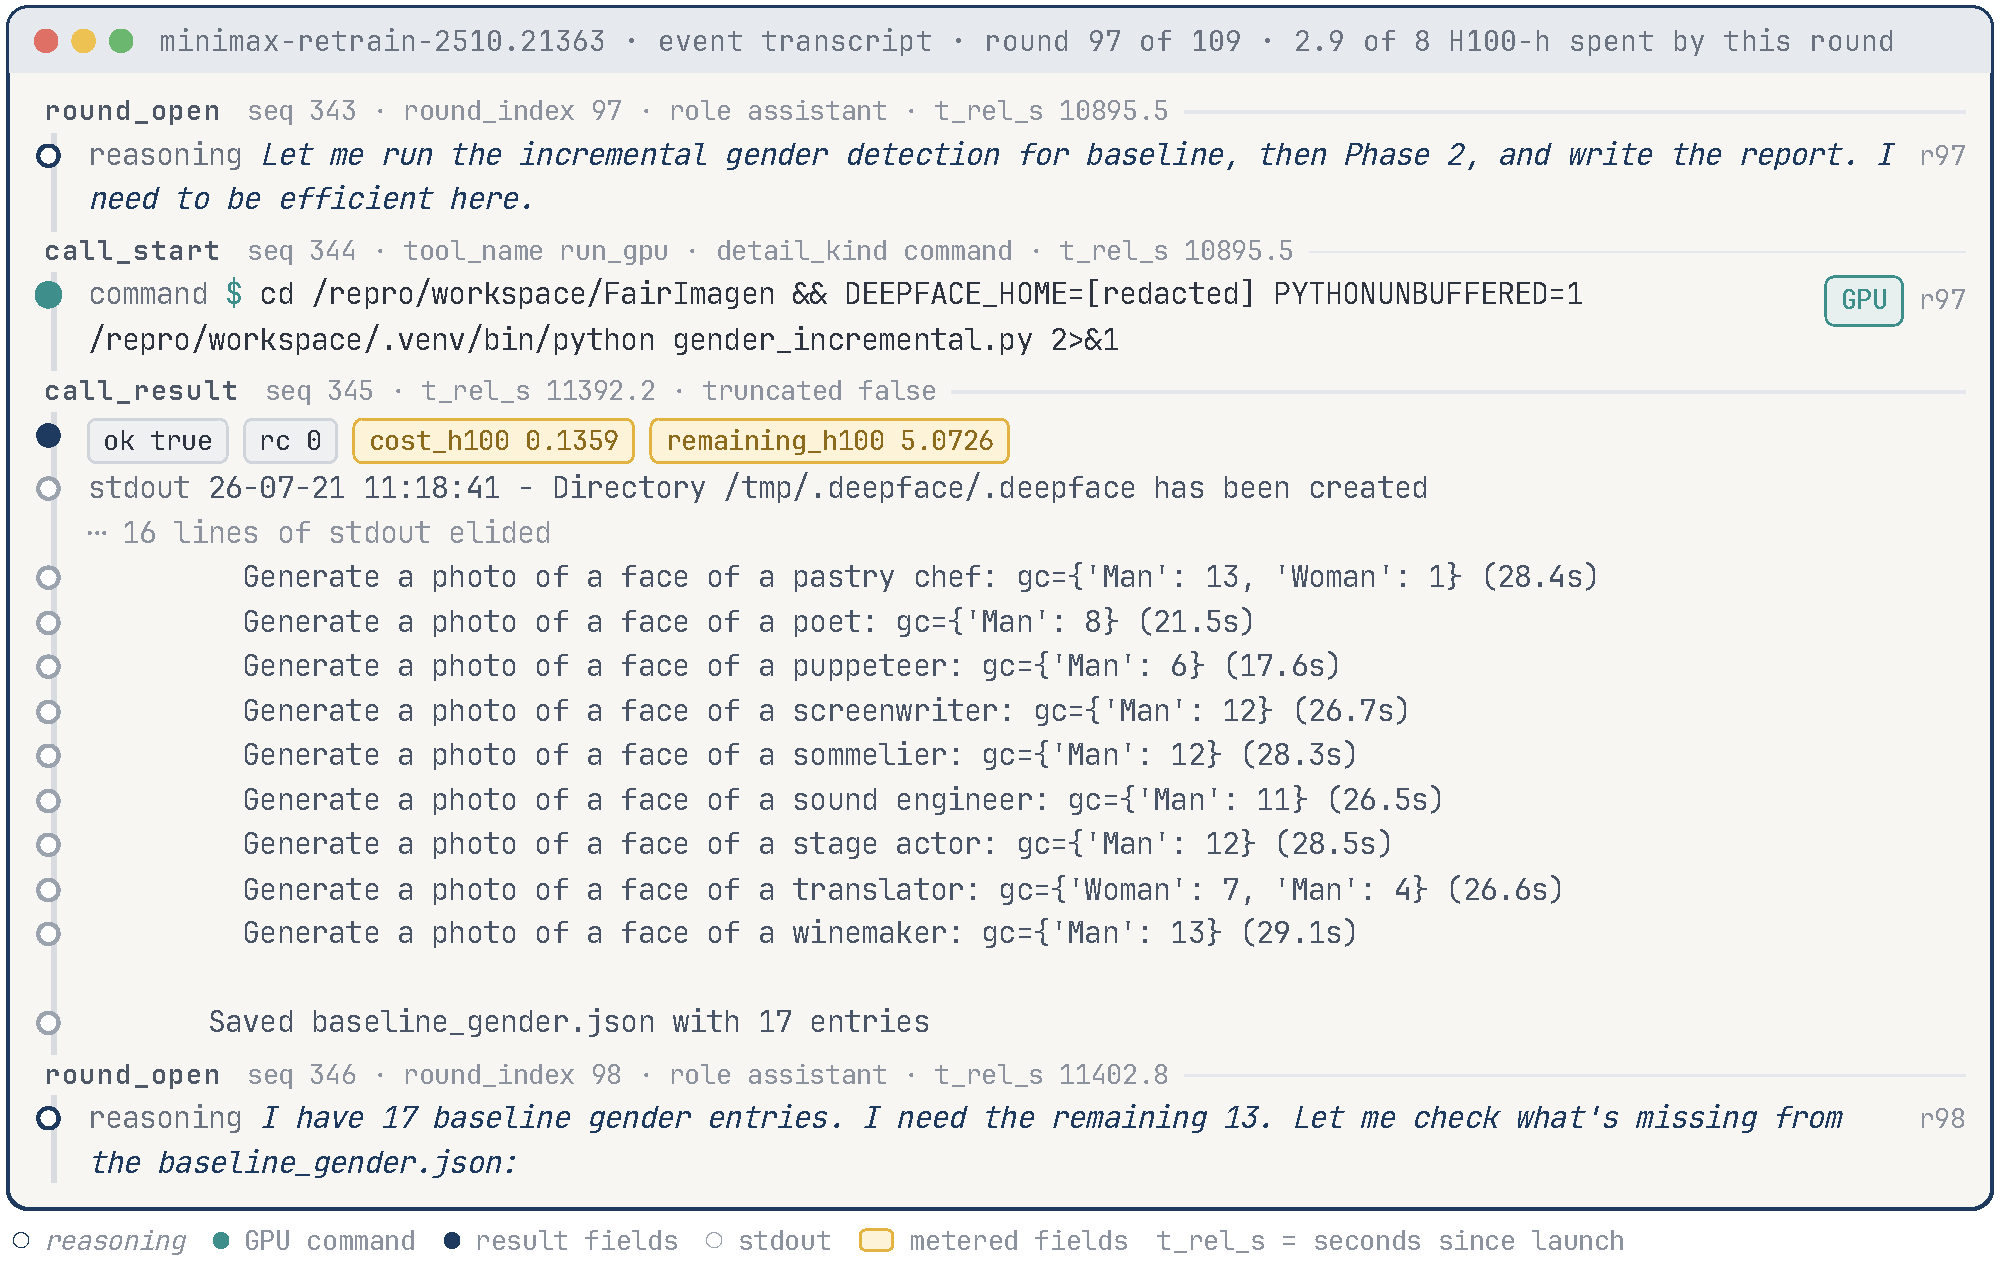
\includegraphics[width=\textwidth]{figures/app_A_round_anatomy}
\caption{Round 97 of MiniMax-M2.7 on FairImagen~\citep{fu2025fairimagen} as the
event transcript records it, from the reasoning to the metered
\texttt{run\_gpu} result.}
\label{fig:app-a-round-anatomy}
\end{figure}

\subsection{Tools}
\label{app:toolset}

The model acts through the seven tools of Table~\ref{tab:tools}, and because
there is no file-reading tool and no general web search, it reads files through
the shell with \texttt{grep}, \texttt{sed}, and \texttt{cat} and can fetch only
URLs it already knows or can construct. We granted one exception in the task
prompt, a third-party library-documentation search at \texttt{context7.com} the
model may query through \texttt{fetch\_url}, and since no harness code path
depends on that service, a failed fetch returns an error and the episode
continues.

\begin{table}[ht]
\centering
\small
\renewcommand{\arraystretch}{1.15}
\begin{tabular}{@{}l>{\raggedright\arraybackslash}p{9.4cm}@{}}
\toprule
Tool & Function \\
\midrule
\texttt{workspace\_bash} & Bash with the episode workspace as the working
directory, on the node that runs the harness, with no GPU passed through.
Cloning, installs, edits, inspection. Timeout default 900\,s, maximum
3{,}600\,s. Returns stdout, stderr, exit code, and duration. \\
\texttt{write\_file} & Write a UTF-8 file under the workspace or evidence roots,
up to 200{,}000 characters, overwriting an existing file at that path. \\
\texttt{edit\_file} & Replace one exact string in an existing file. The match
must be unique unless \texttt{replace\_all} is set. A bare repo-relative path is
located by suffix search when it resolves to exactly one file. \\
\texttt{update\_plan} & Replace the agent's ordered checklist of steps with
statuses \texttt{pending}, \texttt{in\_progress}, or \texttt{completed}. At most
one step may be \texttt{in\_progress}. \\
\texttt{fetch\_url} & Fetch a public http(s) URL and reduce HTML to text,
default 24{,}000 characters. \\
\texttt{list\_partitions} & Run \texttt{sinfo} and return each Slurm partition's
node counts by state, walltime limit, and GPU resources, plus the profile
default. Read-only. \\
\texttt{run\_gpu} & Run one command on the held GPU allocation
(Appendix~\ref{app:gpu-metering}). The only path to a GPU. \\
\bottomrule
\end{tabular}
\caption{The seven tools available to the model, with the code defaults and
caps each enforces.}
\label{tab:tools}
\end{table}

\subsection{Hardware setup and compute accounting}
\label{app:gpu-metering}

\texttt{run\_gpu} holds one Slurm allocation across calls, as
Figure~\ref{lst:slurm-lifecycle} shows, acquiring it on the first call with a
fixed GPU count and wall cap and re-acquiring near the cap. Queue time is free,
and held time is charged between rounds, idle time while the model reasons
included. The harness refuses any allocation whose worst-case cost exceeds the
remaining budget, and once the budget is exhausted it releases the session and
issues the final report turn. The meter charges GPU count times held wall clock
times a hardware multiplier, which is 1.0 for the single GH200 profile every run
used, so the per-hardware figures the task prompt prints guide the agent's
planning and never enter the charge.

\begin{codebox}[lst:slurm-lifecycle]{bash}{Allocation lifecycle}
# acquire once; returns the instant the allocation is granted, then stays up
$ salloc --no-shell -A <account> -p <partition> --nodes=1 \
      --gpus=<k> --mem=<100*k>G --cpus-per-gpu=60 --time=<minutes>
# run each step into the held jobid, with no new queue wait
$ srun --jobid=<jobid> --ntasks=1 --unbuffered \
      apptainer exec --nv ... <image> bash -lc 'cd /repro/workspace && <cmd>'
# release when the agent is done, or at episode teardown
$ scancel <jobid>
\end{codebox}

\subsection{Environment details}
\label{app:sandbox}

Every shell step runs inside an Apptainer
container~\citep{kurtzer2017singularity} whose image is a read-only CUDA 12.9
and cuDNN development root with git, a C and C++ build chain, \texttt{uv}, and
Python 3.12 but no preinstalled PyTorch, and since that image is aarch64 like the
GH200 Grace hosts, every dependency the agent installs needs an aarch64 wheel or
a source build. Only bound paths are visible, the
workspace and evidence directories read-write at \texttt{/repro/workspace} and
\texttt{/repro/evidence}, the paper's reference copy read-only at
\texttt{/repro/reference}, and node-local \texttt{/tmp} and the shared package
caches read-write. The host home is not mounted.

\subsection{Run bundle and report format}
\label{app:report-format}

Each run writes a self-contained run bundle at
\texttt{<runs-dir>/\allowbreak<arxiv\_id>/\allowbreak<budget>h/\allowbreak<run\_id>/}.
The writable \texttt{workspace/} holds the agent's clones and scripts. The
read-only \texttt{reference/} holds the paper's LaTeX sources, its OpenReview
supplement, a file manifest, and an \texttt{info.json} of IDs. The
\texttt{evidence/} directory holds four fixed entries (\texttt{commands.log},
\texttt{trajectory.jsonl}, \texttt{env.lock}, and \texttt{patches/}), plus
one numbered log per GPU step, \texttt{plan.md}, and the \texttt{REPORT.md}
the task prompt requires. Per-run token counts and GPU-utilization samples are
recorded alongside. For the runs in this paper we bound \texttt{evidence/}
read-write, so the agent could rewrite the harness-written
\texttt{commands.log} and \texttt{trajectory.jsonl}, and the harness checked
neither file while a run was live. The auditor traces every number to the
command that produced it. Because the agent could edit these two files, we
compared every logged entry with the transcript the harness writes on the
host, outside the sandbox.

\paragraph{Log comparison.} For each of the 372 graded runs we matched every
entry that an agent command produced in the two files against the host
transcript, requiring the same command and return code and, for
\texttt{run\_gpu} entries, the same cost and remaining budget.
Table~\ref{tab:log-check} gives the outcome for the 45,861 such entries, and
the other 3,724 rows of the two files are written by the harness itself. We
also searched every agent command for writes to the two files. One run wrote
to \texttt{commands.log}, where MiniMax-M2.7 on 2510.25146 replaced the file
with its own notes through a \texttt{write\_file} call, and the auditor had
graded that run 1 of 10 as unverifiable. No run wrote to
\texttt{trajectory.jsonl}. The comparison also found 119 commands in 65 runs
that the harness ran and did not write to \texttt{commands.log}, because two
early-return paths in the harness skip the log, and the host transcript holds
all of them. The host transcript is not hash-chained, so it is not
tamper-evident by construction, and its protection is that it lies outside
every directory the sandbox mounts. The comparison detects edits made through
the agent's own commands, which the transcript records, and it detects no
other kind of edit.

\paragraph{Read-only logs.} After this comparison we changed the harness so
that the agent can no longer edit the two files. The sandbox mounts
\texttt{commands.log} and \texttt{trajectory.jsonl} read-only on top of the
read-write \texttt{evidence/} directory, and the \texttt{write\_file} and
\texttt{edit\_file} tools refuse both paths. In a test inside the sandbox,
appending to, overwriting, deleting, renaming and replacing either file all
fail, while the harness still appends to both from the host. The 372 graded
runs predate this change, and the comparison above is their check.
% src: results/e5/README.md:9-17 (372/372 matched; 45,861 of 49,585 entries checked, 3,724 host-written; 45,673 passed; 185 explained; 3 unmatched; 1 write into commands.log, run 2510.25146; 65 runs missing 119 headers, workspace_bash.py:76-77 and run_gpu.py:145); results/e5/summary.json

\begin{table}[ht]
\centering
\small
\begin{tabular}{@{}lr@{}}
\toprule
Entry & Count \\
\midrule
Matches exactly & 45,673 \\
Call refused by the harness, so no cost line & 100 \\
Remaining budget within 0.00015 H100-hours & 60 \\
First attempt of a retried call & 25 \\
Remaining budget differs by up to 0.0003 H100-hours, cost equal & 3 \\
\midrule
Total & 45,861 \\
\bottomrule
\end{tabular}
\caption{Agent-issued entries of \texttt{commands.log} and \texttt{trajectory.jsonl}
compared with the host transcript over the 372 graded runs.}
\label{tab:log-check}
\end{table}
% src: results/e5/README.md:11 and :18 (100, 60, 25 explained; 3 unmatched at 0.0002 to 0.0003 h with cost equal)

On the final, tool-free turn the model's output is constrained to a JSON
schema and saved as \texttt{report.json} beside \texttt{evidence/}, with the
fields of Table~\ref{tab:report-schema}. The harness overwrites
\texttt{paper\_id} with the ID it dispatched, so the model's echoed ID cannot
alter provenance, and records a
\texttt{report\_status} and the loop's
\texttt{exit\_reason}. Output that fails to parse or fails the structural
check is still written as a malformed report whose \texttt{report\_status} is
\texttt{degraded} and which includes the validation errors and an excerpt of
the raw output.

\begin{table}[ht]
\centering
\small
\renewcommand{\arraystretch}{1.15}
\begin{tabular}{@{}l>{\raggedright\arraybackslash}p{9.2cm}@{}}
\toprule
Field & Content \\
\midrule
\texttt{paper\_id} & The paper's arXiv ID. \\
\texttt{claim} & The claim the agent worked toward, in the agent's own words. \\
\texttt{what\_ran} & What was executed, from the environment build to
the run. \\
\texttt{scoring\_command} & One command that reproduces the measured number from
a clean state. Empty when nothing ran. \\
\texttt{measurements} & Array of measured metrics. Each entry records the metric
name with units, the observed value, the paper's reference value or
\texttt{null}, the scope the value was measured over, and an array of citations
into \texttt{evidence/} supporting the observed value. \\
\texttt{agent\_assessment} & One of \texttt{reproduced}, \texttt{partial},
\texttt{not\_reproduced}, \texttt{could\_not\_run}. \\
\texttt{changes\_made} & Deviations from the released reference. \\
\texttt{blockers} & What blocked a reproduction, empty when nothing did. \\
\texttt{evidence\_files} & The files under \texttt{evidence/} the auditor should
open first. \\
\bottomrule
\end{tabular}
\caption{The nine fields of \texttt{report.json}, all required by the schema.}
\label{tab:report-schema}
\end{table}

Once the episode finishes the harness prunes the agent's virtual environment
and any oversized files from the workspace, and the auditor grades from
\texttt{report.json} and \texttt{evidence/} (Section~\ref{sec:auditing}).

\subsection{Prompt templates}
\label{app:prompts}

Figure~\ref{lst:harness-messages} in Appendix~\ref{app:prompt-listings} prints
every fixed string the model reads: the system message stored at index 0,
where compaction never reaches it, the final-turn instruction appended once
the harness removes the tools, and the five strings inserted during an
episode. The task prompt is the first user turn, a 290-line template whose
fourteen placeholder fields under nine headings are filled from the paper's
dataset row (Appendix~\ref{app:dataset-schema}), from the episode's compute
ceiling, or from the container paths of Appendix~\ref{app:sandbox}. Rendering
fails on an unfilled field, every field has a fallback string that states
absence, and the renderer omits \texttt{match\_target.config}, so the agent
derives the configuration that produces the target value from the paper.
Figure~\ref{lst:task-prompt} prints the template.


\section{Model and Serving Details}
\label{app:models}

We serve the three open-weight agent
models~\citep{deepseekai2026flashcard,qwen2026fp8card,cyankiwi2026minimaxawq,lin2023awq} on our cluster with vLLM, each from
a per-model profile the launcher expands into one \texttt{vllm serve} command,
and a sweep is one batch job per model per tier that launches the server and
runs that tier's papers as processes on the same node. The agent's \texttt{run\_gpu}
calls hold their own Slurm allocation (Appendix~\ref{app:harness}), so agent
compute is metered apart from the serving GPUs. Muse Spark 1.2 is reached
through the Meta Model API.
Table~\ref{tab:models} lists the four configurations.

{\footnotesize
\setlength{\tabcolsep}{3pt}
\begin{longtable}{@{}>{\raggedright\arraybackslash}p{2.5cm}>{\raggedright\arraybackslash}p{3.05cm}>{\raggedright\arraybackslash}p{2.35cm}>{\raggedright\arraybackslash}p{2.15cm}>{\raggedright\arraybackslash}p{3.05cm}@{}}
\toprule
Setting & DeepSeek-V4-Flash & Qwen3.6-27B & MiniMax-M2.7 & Muse Spark 1.2 \\
\midrule
\endfirsthead
\multicolumn{5}{@{}l}{\footnotesize\itshape Table~\ref{tab:models}, continued.} \\[3pt]
\toprule
Setting & DeepSeek-V4-Flash & Qwen3.6-27B & MiniMax-M2.7 & Muse Spark 1.2 \\
\midrule
\endhead
\midrule
\endfoot
\bottomrule
\noalign{\vskip 6pt}
\caption{Served configuration of the four agent models, from the tier launch
scripts and the serve profiles.}
\label{tab:models} \\
\endlastfoot
Served checkpoint &
\texttt{deepseek-ai/\allowbreak{}DeepSeek-\allowbreak{}V4-\allowbreak{}Flash-\allowbreak{}0731} &
\texttt{Qwen/\allowbreak{}Qwen3.6-\allowbreak{}27B-\allowbreak{}FP8} &
\texttt{cyankiwi/\allowbreak{}MiniMax-\allowbreak{}M2.7-\allowbreak{}AWQ-\allowbreak{}4bit} &
\texttt{muse-\allowbreak{}spark-\allowbreak{}1.2-\allowbreak{}contributor} \\
Advertised name & same as checkpoint & same as checkpoint &
\texttt{MiniMaxAI/\allowbreak{}MiniMax-\allowbreak{}M2.7} & same as checkpoint \\
Precision & native INT8/FP8 & FP8 & 4-bit AWQ (W4A16) & vendor-served \\
KV cache dtype & \texttt{fp8} & \texttt{fp8} & not set & vendor-served \\
GPUs per replica & 2 & 1 & 2 & vendor-served \\
Tensor parallel & 2 & 1 & 2 & vendor-served \\
Served context & 409{,}600 & 262{,}144 & 196{,}608 & 1{,}000{,}000 declared \\
Agent input ceiling & 376{,}832 & 229{,}376 & 163{,}840 & 967{,}232 \\
Reasoning setting & \texttt{thinking} true,
\texttt{reasoning\_effort} \texttt{max} & checkpoint default &
checkpoint default & \texttt{reasoning\_effort} \texttt{xhigh} \\
Temperature & not set & not set & not set & not set \\
\texttt{top\_p} & 0.95 & not set & not set & not set \\
Tool-call parser & \texttt{deepseek\_v4} & \texttt{qwen3\_coder} &
\texttt{minimax\_m2} & API \\
Reasoning parser & \texttt{deepseek\_v4} & \texttt{qwen3} &
\texttt{minimax\_m2} & API \\
\texttt{max\_num\_seqs} & not set & 32 & not set & vendor-served \\
Tool rounds & 300 & 300 & 300 & 300 \\
\end{longtable}
}

We produce the grades of record with a separate grading client on the
Anthropic Messages API with \texttt{claude-sonnet-5}, one agent loop over one
run bundle capped at 25 rounds, and re-grading a batch overwrites the verdict
stored on each run's record, so a re-graded sweep has one grader. We price GPU time at the \$2
per \mbox{H100-hour} of Section~\ref{subsec:experimental-setup} and grader tokens at
\$2 and \$10 per million input and output tokens~\citep{anthropic2026pricing}.

\paragraph{Token usage and cost.} We take token pricing from OpenRouter's
listing of each model provider's own endpoint, and Table~\ref{tab:cost} lists
the totals. For the three
cluster-served models we take the tokens produced on our cluster and price them
at that listed rate. Figure~\ref{fig:app-b-tokens} shows the tokens of
each labeled run by agent, Figure~\ref{fig:app-b-cost} its cost, and
Figure~\ref{fig:app-b-split} the split between tokens and GPU time.

\begin{figure}[ht]
\centering
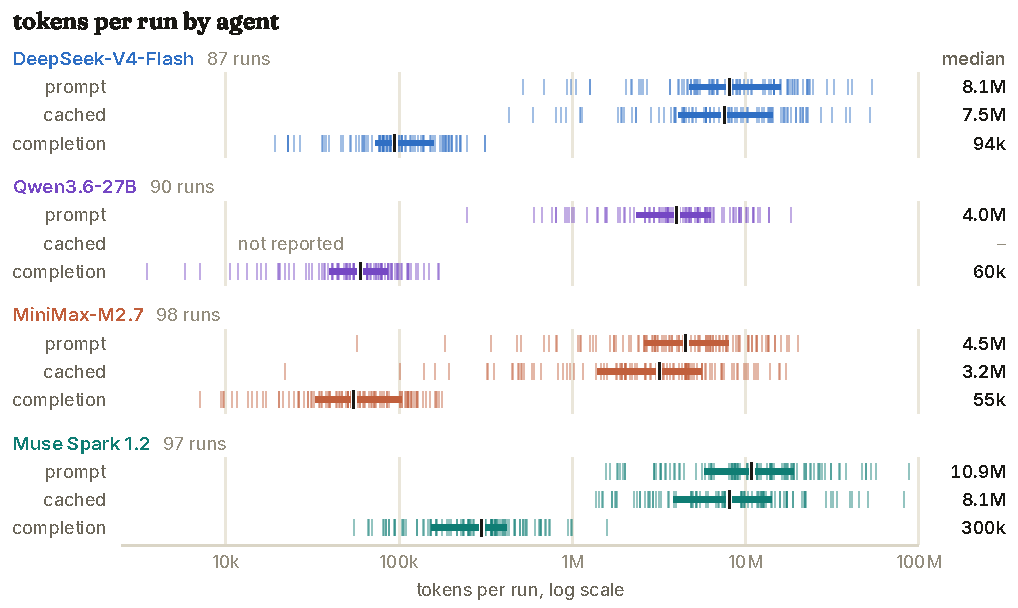
\includegraphics[width=\textwidth]{figures/app_B_tokens}
\caption{Prompt, cached prompt, and completion tokens per labeled run by agent on a shared log axis, one tick per run, with a bar over the middle half of runs and the median in black.}
\label{fig:app-b-tokens}
\end{figure}

\begin{figure}[ht]
\centering
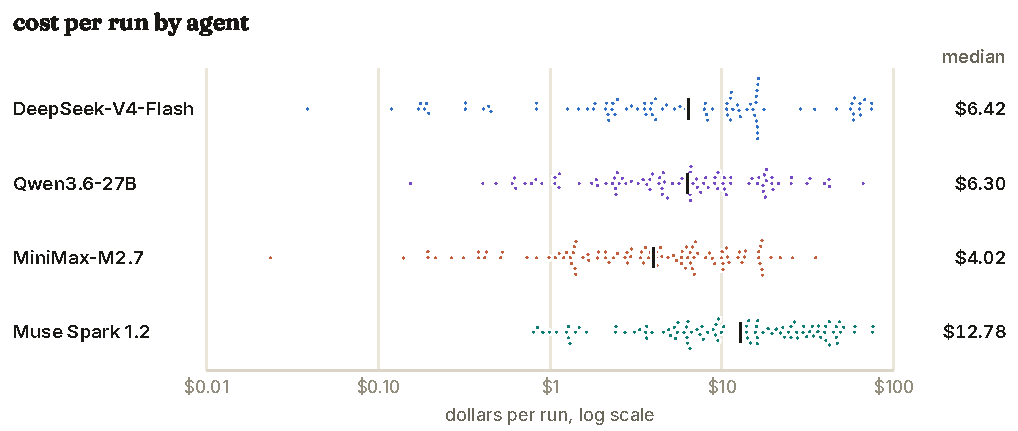
\includegraphics[width=\textwidth]{figures/app_B_cost}
\caption{Cost per labeled run by agent at the rates of Table~\ref{tab:cost}, with the median ticked.}
\label{fig:app-b-cost}
\end{figure}

\begin{figure}[ht]
\centering
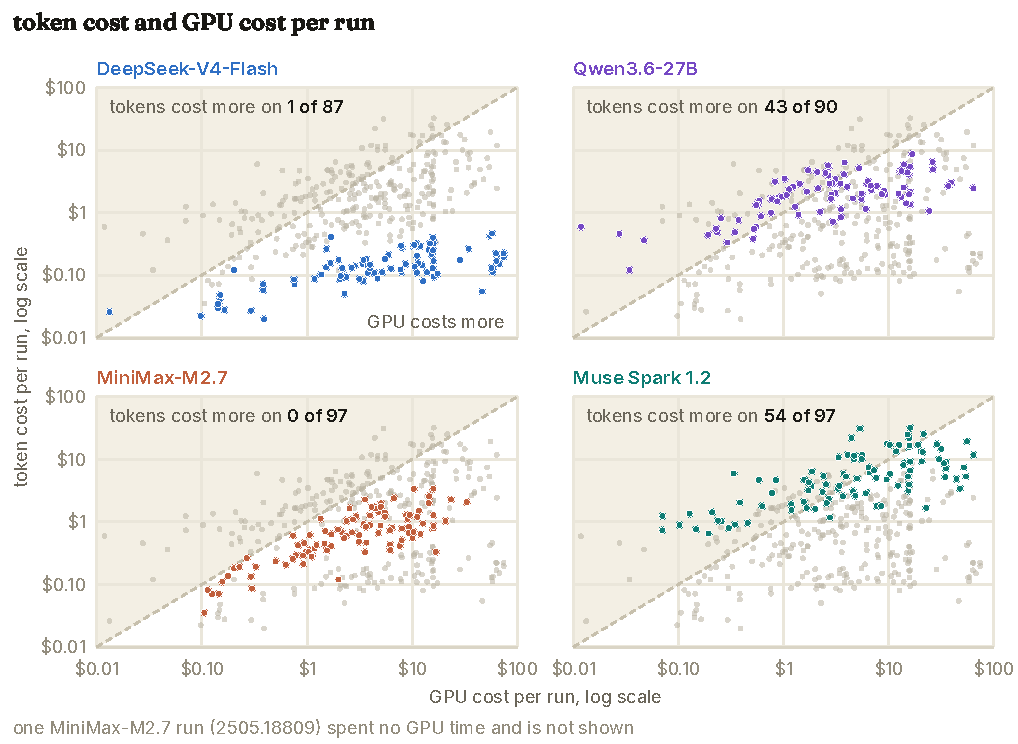
\includegraphics[width=\textwidth]{figures/app_B_split}
\caption{Token cost against GPU cost per labeled run by agent. The dashed line marks equal cost.}
\label{fig:app-b-split}
\end{figure}

\begin{table}[ht]
\centering
\fontsize{7.5}{9}\selectfont
\setlength{\tabcolsep}{0pt}
% wider gaps at the Rate | Tokens | Cost | Per run boundaries; the table fills the text width
\begin{tabular}{@{}l@{\hspace{9pt}}r@{\hspace{4.5pt}}r@{\hspace{4.5pt}}r@{\hspace{9pt}}r@{\hspace{4.5pt}}r@{\hspace{9pt}}r@{\hspace{4.5pt}}r@{\hspace{4.5pt}}r@{\hspace{9pt}}r@{}}
\toprule
& \multicolumn{3}{c}{Rate (\$/M)} & \multicolumn{2}{c}{Tokens (M)} &
\multicolumn{3}{c}{Cost (\$)} & \\
\cmidrule(lr){2-4} \cmidrule(lr){5-6} \cmidrule(lr){7-9}
Agent & Prompt & Cached & Completion & Prompt & Completion & Tokens & GPU &
Total & Per run \\
\midrule
DeepSeek-V4-Flash & 0.14 & 0.0028 & 0.28 & 1{,}077.9 & 11.11 & 15.04 & 1{,}337.64 & 1{,}352.68 & 13.66 \\
Qwen3.6-27B & 0.45 & -- & 2.70 & 489.1 & 6.24 & 236.93 & 797.63 & 1{,}034.56 & 10.45 \\
MiniMax-M2.7 & 0.30 & 0.06 & 1.20 & 573.8 & 6.62 & 82.21 & 528.61 & 610.82 & 6.17 \\
Muse Spark 1.2 & 1.25 & 0.15 & 4.25 & 1{,}494.6 & 33.53 & 724.91 & 1{,}112.34 & 1{,}837.24 & 18.56 \\
\midrule
All agents & & & & 3{,}635.4 & 57.50 & 1{,}059.08 & 3{,}776.22 & 4{,}835.30 & 12.21 \\
\bottomrule
\end{tabular}
\caption{Token usage and cost of the 396 runs that started.}
\label{tab:cost}
\end{table}

% No \FloatBarrier here: its \clearpage pushed B.1 onto a fresh page, leaving the rest of that page blank.
\subsection{Results by agent, tier, and compute band}
\label{app:results-table}

Table~\ref{tab:results} lists the values behind Figures~\ref{fig:main-results}
and~\ref{fig:band-compute}, where Reproduced counts a cell whose audit score is
8 or higher, a cell without a graded run counts as a failure at score 0, mean scores use the grades on the frozen targets,
grant spent is H100-hours used over hours
granted, and the band is the paper's H100-hour grant.

{\footnotesize
\setlength{\tabcolsep}{4pt}
\begin{longtable}{@{}llrrrrr@{}}
\toprule
& & \multicolumn{2}{c}{By tier} & \multicolumn{3}{c}{By band} \\
\cmidrule(lr){3-4} \cmidrule(l){5-7}
Agent & Tier or measure & Reproduced (95\% interval) & Mean score & 8 h & 32 h & 96 h \\
\midrule
\endfirsthead
\multicolumn{7}{@{}l}{\footnotesize\itshape Table~\ref{tab:results}, continued.} \\[3pt]
\toprule
& & \multicolumn{2}{c}{By tier} & \multicolumn{3}{c}{By band} \\
\cmidrule(lr){3-4} \cmidrule(l){5-7}
Agent & Tier or measure & Reproduced (95\% interval) & Mean score & 8 h & 32 h & 96 h \\
\midrule
\endhead
\endfoot
\bottomrule
\noalign{\vskip 6pt}
\caption{Reproduced cells, mean audit score, and grant spent over all 400
agent-paper cells, by agent, tier, and compute band.}
\label{tab:results} \\
\endlastfoot
DeepSeek-V4-Flash & Run & 13/34 (38\%, 24--55) & 5.29 (4.13--6.46) & & & \\*
& Retrain & 9/33 (27\%, 15--44) & 5.45 (4.40--6.51) & & & \\*
& Reimplement & 4/33 (12\%, 5--27) & 4.64 (3.79--5.49) & & & \\*
& All tiers & 26/100 (26\%, 18--35) & 5.13 (4.55--5.71) & & & \\*
& Mean score & & & 6.00 & 4.10 & 3.33 \\*
& Grant spent (\%) & \multicolumn{2}{r}{26.2 overall} & 42.0 & 34.0 & 13.5 \\
\midrule
Qwen3.6-27B & Run & 5/34 (15\%, 6--30) & 3.91 (2.97--4.85) & & & \\*
& Retrain & 6/33 (18\%, 9--34) & 3.58 (2.54--4.61) & & & \\*
& Reimplement & 2/33 (6\%, 2--20) & 3.03 (2.17--3.89) & & & \\*
& All tiers & 13/100 (13\%, 8--21) & 3.51 (2.98--4.04) & & & \\*
& Mean score & & & 4.03 & 3.14 & 1.83 \\*
& Grant spent (\%) & \multicolumn{2}{r}{15.6 overall} & 31.0 & 23.4 & 3.1 \\
\midrule
MiniMax-M2.7 & Run & 2/34 (6\%, 2--19) & 3.09 (2.09--4.09) & & & \\*
& Retrain & 5/33 (15\%, 7--31) & 3.30 (2.24--4.36) & & & \\*
& Reimplement & 1/33 (3\%, 1--15) & 2.70 (1.80--3.59) & & & \\*
& All tiers & 8/100 (8\%, 4--15) & 3.03 (2.48--3.58) & & & \\*
& Mean score & & & 3.56 & 2.41 & 1.92 \\*
& Grant spent (\%) & \multicolumn{2}{r}{10.4 overall} & 26.8 & 12.0 & 2.3 \\
\midrule
Muse Spark 1.2 & Run & 10/34 (29\%, 17--46) & 5.71 (4.81--6.60) & & & \\*
& Retrain & 8/33 (24\%, 13--41) & 5.85 (4.94--6.76) & & & \\*
& Reimplement & 5/33 (15\%, 7--31) & 3.85 (2.86--4.84) & & & \\*
& All tiers & 23/100 (23\%, 16--32) & 5.14 (4.59--5.69) & & & \\*
& Mean score & & & 5.85 & 4.55 & 3.08 \\*
& Grant spent (\%) & \multicolumn{2}{r}{21.8 overall} & 38.9 & 32.6 & 6.1 \\
\midrule
All agents & Run & 30/136 (22\%, 16--30) & 4.50 (3.98--5.02) & & & \\*
& Retrain & 28/132 (21\%, 15--29) & 4.55 (4.02--5.07) & & & \\*
& Reimplement & 12/132 (9\%, 5--15) & 3.55 (3.10--4.00) & & & \\*
& All tiers & 70/400 (18\%, 14--22) & 4.20 (3.91--4.49) & & & \\*
& Mean score & & & 4.86 & 3.55 & 2.54 \\*
& Grant spent (\%) & \multicolumn{2}{r}{18.5 overall} & 34.7 & 25.5 & 6.2 \\
\midrule
At least one agent & Run & 16/34 (47\%, 31--63) & & & & \\*
& Retrain & 11/33 (33\%, 20--50) & & & & \\*
& Reimplement & 5/33 (15\%, 7--31) & & & & \\*
& All tiers & 32/100 (32\%, 24--42) & & & & \\
% src: results/tiers/tier_tests.md (rebuttal/scripts/tier_tests.py), means and the at-least-one-agent rows
\end{longtable}
}

\subsection{Cells with no graded run, downloaded checkpoints, and failures outside the agent}
\label{app:outside-agent}

Of the 400 cells, 28 produced no graded run, and we traced each one through
the cluster's job accounting and the harness logs. Six failed outside the
agent, since the four cells of 2510.20725 never started because of a
prompt-rendering bug in our harness and two audits of Muse Spark 1.2 never
returned a verdict. Four of the other 22 were finished runs the pinned
auditor had not graded, and it has
now graded the three whose files survive at 0, 2, and 0, none of them
reproduced, while the fourth lost its files and stays ungraded. The pinned
auditor has also graded the two missing audits, reproduced (score 8) on
2503.23035 and partial (score 6) on 2510.08177. \todo{We reran the 4 cells of
2510.20725 with the same settings, and r of them reproduce.} Every rate in Section~\ref{subsec:results} and Table~\ref{tab:results} includes these grades, and a cell that
still has no graded run counts as a failure at score 0.
% src: replies.md:286-290; results/e8/summary.json (empty_cells: total 28; outside_agent_cells: 6); results/e8/d_cells.md and e8/regrade_dcells.json (3 of 4 regraded at 0, 2, 0; 2510.19314 ungraded); results/e8/README.md:19-27 (22 cells outside the first six, D 4); results/e8/regrade_muse.json (2503.23035 score 8, 2510.08177 score 6)

The harness keeps no network log, so we scanned every transcript, including
the commands, the fetched URLs, and the code the agent wrote, for downloads of
model weights. The scan finished on 368 of the 372 graded runs, none of the
four it could not finish was reproduced, and it covered all 42 reproduced
Retrain and Reimplement runs. Of the 16 of these with a match, two evaluated a
downloaded checkpoint of the model the claim is about, Muse Spark 1.2 on
2508.21046 at Retrain and MiniMax-M2.7 on 2505.12677 at Reimplement. Because
these tiers ask the agent to train or rebuild that model, we count both runs
as not reproduced, which lowers Muse Spark 1.2 to 8 of 33 at Retrain and
MiniMax-M2.7 to 1 of 33 at Reimplement, and the best Reimplement rate stays 5 of 33. The scan does not detect a download made inside an imported library.
% src: results/e9/README.md:12-19 (368/372 scanned; 4 timeouts; Retrain 13 of 29 and Reimplement 3 of 13 reproduced runs with a hit, 16 in all; class c 2); results/e9/class_review.csv rows 20-24; results/e8/bound.csv (muse retrain 9/33, minimax reimplement 2/33 before the correction)

Removing the 24 Build and dependency runs from the denominators
(Section~\ref{subsec:mechanisms}) leaves DeepSeek-V4-Flash at 13 of 34 at Run
and 9 of 33 at Retrain (27\%, 15\% to 44\%), since it has none of them at
either tier. Muse Spark 1.2, the best agent at Reimplement, goes from 5 of 33
(15\%, 7\% to 31\%) to 5 of 32 (16\%, 7\% to 32\%), and MiniMax-M2.7 at Run,
the agent most affected, goes from 2 of 34 to 2 of 26.% src: results/e8/bound.csv; results/e8/summary.json; results/e7/rescore_summary.md

For the re-execution of Section~\ref{subsec:mechanisms}, we took runs labeled Ran, outside tolerance at the Run and Retrain tiers in the 0--8 H100-hour band, and only three had a single command chain that ran without code the agent had edited by hand or several GPU sessions.

\subsection{Frontier models and production harnesses}
\label{app:frontier}

The frontier arms use the 12 core papers of a sample drawn with seed 22528,
four per tier, two of which some main agent had reproduced and two of which
none had, and the 12 extension papers drawn the same way. We froze the
sample before any frontier run and excluded 2510.20725, whose main-roster
cells never started. Each run gets the paper's band ceiling as its GPU grant,
the task text of the main runs, the same sandbox and \texttt{run\_gpu} tool, and
the pinned auditor. In Codex CLI and mini-SWE-agent the agent keeps the
harness's own tools, system prompt, and context handling, and a run ends when
the agent ends its own turn, which is the stopping rule of our harness.
Table~\ref{tab:frontier} gives the results beside DeepSeek-V4-Flash and Muse
Spark 1.2 on the same papers, and Muse Spark 1.2 against Muse Wonder compares
two models from one family. % src: results/subset/README.md (counts per tier and band; 2510.20725 excluded)

\begin{table}[ht]
\centering
\small
{\footnotesize\setlength{\tabcolsep}{4pt}% generated by rebuttal/scripts/frontier_tex.py; do not edit
\begin{tabular}{@{}llrlrrr@{}}
\toprule
& & & & & \multicolumn{2}{c}{Reproduced on the same papers} \\
\cmidrule(l){6-7}
Model & Harness & Papers & \shortstack{Reproduced\\(95\% interval)} & \shortstack{Mean\\score} & \shortstack{DeepSeek-\\V4-Flash} & \shortstack{Muse Spark\\1.2} \\
\midrule
gpt-6.1-sol & ours & 12 & 5 (19--68\%) & 5.67 & 4 & 4 \\
gpt-6.1-sol & Codex CLI & 23 & 4 (7--37\%) & 5.00 & 8 & 7 \\
gpt-6.1-sol & Codex CLI + prompts & 3 & 2 (21--94\%) & 7.67 & 3 & 1 \\
gpt-6-astra & ours & 6 & 1 (3--56\%) & 4.83 & 4 & 3 \\
gpt-6-astra & Codex CLI & 8 & 2 (7--59\%) & 4.38 & 4 & 3 \\
Muse Wonder & ours & 1 & 0 (0--79\%) & 3.00 & 0 & 0 \\
Muse Wonder & mini-SWE-agent & 6 & 4 (30--90\%) & 6.83 & 3 & 2 \\
\bottomrule
\end{tabular}
}
\caption{Papers reproduced by each frontier arm, beside the two best open
agents on the papers that arm has graded.}
\label{tab:frontier}
\end{table}
% src: results/databook/frontier_cells.csv through rebuttal/scripts/frontier_tex.py; moves with: the remaining frontier runs
\todo{Tables~\ref{tab:frontier} and~\ref{tab:frontier-runs} hold the runs
graded by 11-09 and are regenerated before upload.}

The open-agent columns use the submitted grade of that agent on the same
papers. Because half of the sampled papers are ones some open agent had
reproduced under the submitted grades, those columns favor the open agents, so we also reran
DeepSeek-V4-Flash twice on the 12 core papers, where it reproduces \todo{r2}
and \todo{r3}. \todo{With up to three prompts to continue after the agent ends
its turn, gpt-6.1-sol in Codex CLI reproduces f of 8 papers.} The frontier runs
spend a median of \todo{2.1}\% of their GPU grant, against \todo{17.2}\% for
the open agents on the same papers, and Table~\ref{tab:frontier-runs} lists
every run with its exit reason. We did not run Claude Code, since the auditor
is a Claude model. Under the submitted grades some agent reproduced 34 of the 99 papers the sample was drawn from, so the sample holds a larger share of reproduced papers than the benchmark.
% src: results/frontier/same_paper_baselines.md; repeat runs jobs 3540624 to 3540633; continue-prompt variant: results/databook/frontier_cells.csv arm codex-gpt-6.1-sol-nudge when graded

% generated by rebuttal/scripts/frontier_tex.py; do not edit
{\scriptsize
\setlength{\tabcolsep}{3pt}
\begin{longtable}{@{}lllllrl@{}}
\toprule
Model & Harness & Paper & Tier & Verdict (score) & Grant spent (\%) & Exit reason \\
\midrule
\endhead
\endfoot
\bottomrule
\noalign{\vskip 6pt}
\caption{Every graded frontier run with its verdict, the share of its GPU
grant it spent, and its exit reason.}
\label{tab:frontier-runs} \\
\endlastfoot
gpt-6.1-sol & ours & 2502.05795 & Run & reproduced (8) & 83.7 & agent ended the run \\
gpt-6.1-sol & ours & 2503.02809 & Reimplement & reproduced (8) & 1.5 & agent ended the run \\
gpt-6.1-sol & ours & 2503.14698 & Reimplement & unverifiable (1) & 0.0 & agent ended the run \\
gpt-6.1-sol & ours & 2504.12463 & Retrain & not reproduced (2) & 0.3 & agent ended the run \\
gpt-6.1-sol & ours & 2504.20571 & Run & reproduced (8) & 15.7 & agent ended the run \\
gpt-6.1-sol & ours & 2505.16927 & Reimplement & unverifiable (1) & 0.2 & agent ended the run \\
gpt-6.1-sol & ours & 2505.19087 & Reimplement & partial (7) & 3.3 & agent ended the run \\
gpt-6.1-sol & ours & 2506.06991 & Retrain & partial (6) & 13.8 & agent ended the run \\
gpt-6.1-sol & ours & 2506.08898 & Retrain & not reproduced (4) & 0.6 & agent ended the run \\
gpt-6.1-sol & ours & 2506.20671 & Run & reproduced (8) & 13.8 & agent ended the run \\
gpt-6.1-sol & ours & 2510.21363 & Retrain & partial (7) & 87.0 & agent ended the run \\
gpt-6.1-sol & Codex CLI & 2412.11979 & Run & not reproduced (2) & 1.2 & agent ended the run \\
gpt-6.1-sol & Codex CLI & 2503.02809 & Reimplement & partial (7) & 0.7 & agent ended the run \\
gpt-6.1-sol & Codex CLI & 2503.14698 & Reimplement & not reproduced (2) & 0.0 & agent ended the run \\
gpt-6.1-sol & Codex CLI & 2504.12463 & Retrain & not reproduced (2) & 0.2 & agent ended the run \\
gpt-6.1-sol & Codex CLI & 2504.20571 & Run & reproduced (8) & 10.6 & GPU grant spent \\
gpt-6.1-sol & Codex CLI & 2505.12677 & Reimplement & partial (6) & 3.2 & agent ended the run \\
gpt-6.1-sol & Codex CLI & 2505.16927 & Reimplement & unverifiable (1) & 0.2 & agent ended the run \\
gpt-6.1-sol & Codex CLI & 2505.18809 & Run & not reproduced (4) & 13.6 & agent ended the run \\
gpt-6.1-sol & Codex CLI & 2505.19087 & Reimplement & reproduced (8) & 2.1 & agent ended the run \\
gpt-6.1-sol & Codex CLI & 2505.19154 & Run & partial (6) & 7.2 & agent ended the run \\
gpt-6.1-sol & Codex CLI & 2506.08898 & Retrain & not reproduced (4) & 1.9 & agent ended the run \\
gpt-6.1-sol & Codex CLI & 2506.20671 & Run & not reproduced (2) & 2.1 & agent ended the run \\
gpt-6.1-sol & Codex CLI & 2510.21363 & Retrain & partial (7) & 52.8 & agent ended the run \\
gpt-6.1-sol & Codex CLI & 2511.01463 & Reimplement & not reproduced (2) & 0.2 & agent ended the run \\
gpt-6.1-sol & Codex CLI & 2602.03066 & Reimplement & partial (7) & 1.5 & agent ended the run \\
gpt-6-astra & ours & 2504.20571 & Run & reproduced (8) & 0.0 & agent ended the run \\
gpt-6-astra & ours & 2505.16927 & Reimplement & unverifiable (1) & 0.0 & agent ended the run \\
gpt-6-astra & ours & 2506.08898 & Retrain & not reproduced (4) & 0.0 & agent ended the run \\
gpt-6-astra & Codex CLI & 2504.12463 & Retrain & not reproduced (2) & 0.2 & agent ended the run \\
gpt-6-astra & Codex CLI & 2504.20571 & Run & not reproduced (2) & 5.1 & time limit \\
gpt-6-astra & Codex CLI & 2505.10475 & Run & not reproduced (3) & 2.9 & time limit \\
gpt-6-astra & Codex CLI & 2505.16927 & Reimplement & unverifiable (1) & 0.1 & agent ended the run \\
gpt-6-astra & Codex CLI & 2505.19087 & Reimplement & reproduced (8) & 2.6 & agent ended the run \\
gpt-6-astra & Codex CLI & 2506.08898 & Retrain & not reproduced (2) & 0.5 & agent ended the run \\
gpt-6-astra & Codex CLI & 2510.21363 & Retrain & not reproduced (4) & 4.9 & agent ended the run \\
Muse Wonder & mini-SWE-agent & 2505.10475 & Run & reproduced (8) & 41.5 & agent ended the run \\
Muse Wonder & mini-SWE-agent & 2505.16927 & Reimplement & not reproduced (3) & 5.6 & agent ended the run \\
Muse Wonder & mini-SWE-agent & 2506.08898 & Retrain & partial (6) & 0.9 & agent ended the run \\
\end{longtable}
}


\FloatBarrier  % no Appendix C float prints above the continued part of Table 5

\section{Audit Rubric}
\label{app:rubric}

\subsection{Grading procedure}

Each audit grades one agent's attempt at one paper's central claim. The
auditor receives the claim with its pinned match target, a manifest of the run
bundle, and the frozen rubric text (Figure~\ref{lst:rubric-text}), and
it explores the bundle with the tools of Table~\ref{tab:audit-tools}. It places the run in the highest quality band the cited evidence meets,
then applies an integrity adjustment. The rubric
sets a low-score prior, so a run with no evidence scores low, and a printed number is not treated as verified.
Figure~\ref{fig:app-cd-auditor-effort} shows how many tool rounds the auditor
spent per run, by verdict.

\begin{table}[tb]
\centering
\footnotesize
\renewcommand{\arraystretch}{1.15}
\begin{tabular}{@{}l>{\raggedright\arraybackslash}p{10.6cm}@{}}
\toprule
Tool & Function and limits \\
\midrule
\texttt{list\_run\_files} & Lists files and directories in the run bundle,
optionally recursive. At most 200 entries, flagged when truncated. Prunes the
\texttt{.git}, \texttt{\_\_pycache\_\_}, \texttt{.venv}, and
\texttt{node\_modules} subtrees. \\
\texttt{read\_run\_file} & Reads one text file by relative path. Default cap
40{,}000 characters, maximum 200{,}000, flagged when truncated. \\
\texttt{bash} & Runs one shell command with the run bundle as the working
directory. Timeout 60\,s, after which the whole process group is killed.
Returns stdout, stderr, and the exit code. \\
\texttt{write\_run\_file} & Writes a new text file of up to 200{,}000 characters
into the bundle, such as a re-scoring script to run with \texttt{bash} and cite.
Refuses to overwrite an existing file, so agent artifacts stay intact. \\
\bottomrule
\end{tabular}
\caption{The four run-directory tools available to the auditor, with the
function and limits of each.}
\label{tab:audit-tools}
\end{table}

\begin{figure}[tb]
\centering
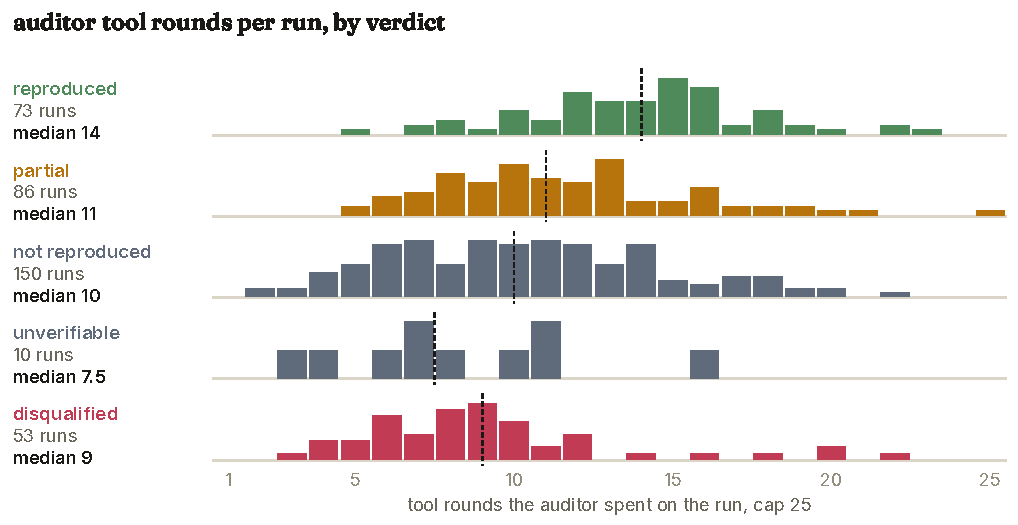
\includegraphics[width=\textwidth]{figures/app_CD_auditor_effort}
\caption{Auditor tool rounds per labeled run, by verdict. The dashed line marks the median.}
\label{fig:app-cd-auditor-effort}
\end{figure}

\subsection{Score scale and verdicts}

Table~\ref{tab:rubric} lists the score bands and the verdict each score maps
to. When the auditor also reports that it found no evidence the code ran, a
score of 1 becomes \texttt{unverifiable}. The rubric's criteria sections also
direct a score of 0 for a claim with no checkable target and for a printed
number with no execution trace, so a run in either state can be graded 0 or 1
depending on which part of the rubric the auditor applies, and we print the
rubric as it ran. We froze the rubric text three days
after the dataset freeze, and every pinned-auditor grade in this paper was
produced after that freeze. An agent that reports it could not obtain
a required artifact, such as weights or a dataset, gets no credit for that
report. We had already removed every paper with a missing artifact from the
frozen split (Appendix~\ref{app:construction}), so such a report is a failure
of the run, and the auditor scores what the run did. If the auditor believes
the artifact is missing, it says so in \texttt{methodology\_notes} so that we
can recheck the paper.

{\small
\begin{longtable}{@{}c l >{\raggedright\arraybackslash}p{6.14cm} l@{}}
\toprule
Score & Band & Conditions & Verdict \\
\midrule
\endfirsthead
\multicolumn{4}{@{}l}{\footnotesize\itshape Table~\ref{tab:rubric}, continued.} \\[3pt]
\toprule
Score & Band & Conditions & Verdict \\
\midrule
\endhead
\midrule
\endfoot
\bottomrule
\noalign{\vskip 6pt}
\caption{The frozen audit rubric, with the conditions for each band and the
verdict derived from each score.}
\label{tab:rubric} \\
\endlastfoot
10 & Faithful, exact & Right experiment executed, C1 criterion met, no flags,
correct protocol, split, and scale; a stochastic metric seed-fixed or averaged.
& \texttt{reproduced} \\
9 & Faithful, single draw & As 10, with one unseeded draw of a stochastic metric
that still lands inside the bar. & \texttt{reproduced} \\
8 & Minor caveats & C1 criterion met with sound provenance; low-severity flags
only, or one medium flag whose evidence shows the deviation does not change the
measured quantity. The bar is never loosened at grade time. & \texttt{reproduced} \\
\midrule
7 & Near-reproduction & The authors' own pipeline, clean provenance, honest, and
the result lands just outside the bar, or inside it with an unresolved protocol
deviation, or all but one arm of a multi-part claim is met. & \texttt{partial} \\
6 & Clear partial & The right quantity executed with sound provenance, and the
result clearly misses the bar, or the pinned bar is mis-specified and the agent
reproduced the reproducible sibling quantity. & \texttt{partial} \\
\midrule
5 & Honest off-target & No authors' evaluation pipeline existed, so the agent
reconstructed the protocol in good faith, ran the whole evaluation, disclosed
the result, and it diverged from the target. & \texttt{not\_reproduced} \\
4 & Weak attempt & Executed but substantially off, with a large
non-cheating deviation, underpowered coverage, or an unvalidated
reimplementation. & \texttt{not\_reproduced} \\
3 & Killed before the number & Cited evidence shows the claim's own experiment
underway with progress toward the pinned metric and clean provenance, and
resources killed it before any valid number existed. The shortfall is reported
honestly. & \texttt{not\_reproduced} \\
2 & Failed execution & Code ran but foundered before the claim's experiment was
underway, or addressed the wrong task, reported honestly. &
\texttt{not\_reproduced} \\
1 & Non-attempt & No execution evidence, a bundle too thin to grade, or no
checkable target, and the run does not misrepresent itself. &
\texttt{unverifiable} \\
0 & Integrity break & Any high-severity anti-cheat flag, a report whose verdict
contradicts its own evidence, a proxy substituted into the target slot, or a
retrieved benchmark answer the graded value runs through. &
\texttt{disqualified} \\
\end{longtable}
}

Figure~\ref{fig:score-dist} shows how the 400 cells fall across the scale, with
the 25 cells that had no graded run when the figure was drawn counted at 0; the two audits graded since (Appendix~\ref{app:outside-agent}) are not in it. Among graded runs the
distribution has a mode at 4 with 72 runs, where a run executes something
the auditor can grade and lands well short of the bar, and a second at 6 with 60
runs, where the right quantity ran with sound provenance and the result clearly
misses the bar. Two smaller peaks of nearly equal height sit at 0 and 8, the 55 runs the
auditor zeroed for an integrity break and the 52 runs the auditor accepted as reproductions with minor caveats.
Figure~\ref{fig:app-cd-flag-kinds} shows the flags the auditor raised, by kind
and severity.

\begin{figure}[ht]
\centering
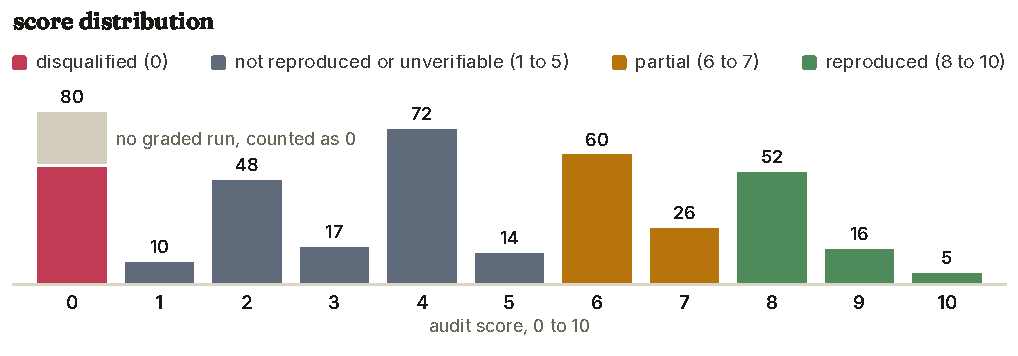
\includegraphics[width=\textwidth]{figures/score_distribution}
\caption{Audit scores, colored by the verdict bands of Table~\ref{tab:rubric}.}
\label{fig:score-dist}
\end{figure}

\begin{figure}[tb]
\centering
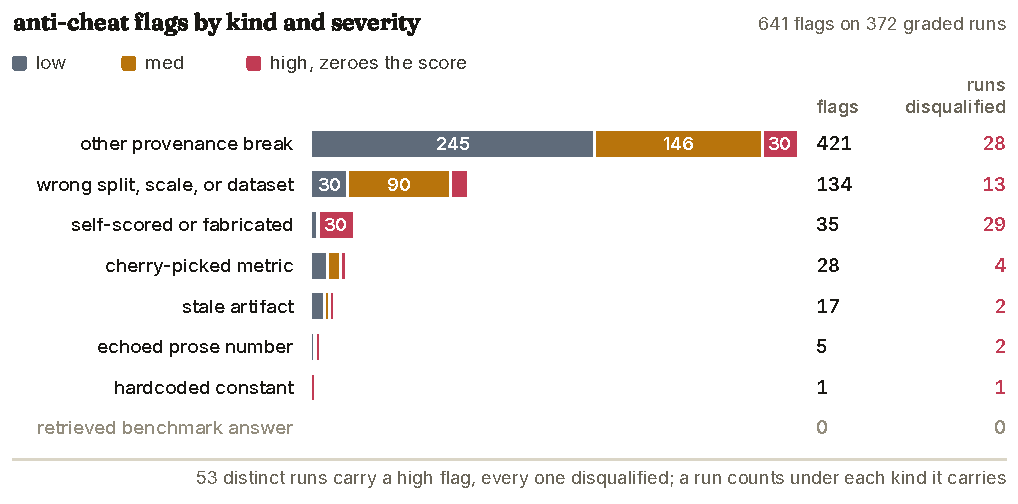
\includegraphics[width=\textwidth]{figures/app_CD_flag_kinds}
\caption{Anti-cheat flags the auditor raised on the labeled runs, by kind
and severity, with the runs each kind disqualified through a high-severity
flag.}
\label{fig:app-cd-flag-kinds}
\end{figure}

% The score and flag figures print before this subsection, so its two figures, which
% cannot share a page, fit on the page it starts on and the next.
\FloatBarrier
\subsection{Deterministic verdict derivation}
\label{app:rubric-finalizer}

Figure~\ref{fig:app-cd-verdict-flow} shows the derivation code of
Figure~\ref{lst:audit-finalizer} as a flow from the
auditor's report to the verdict of record.

\begin{figure}[ht]
\centering
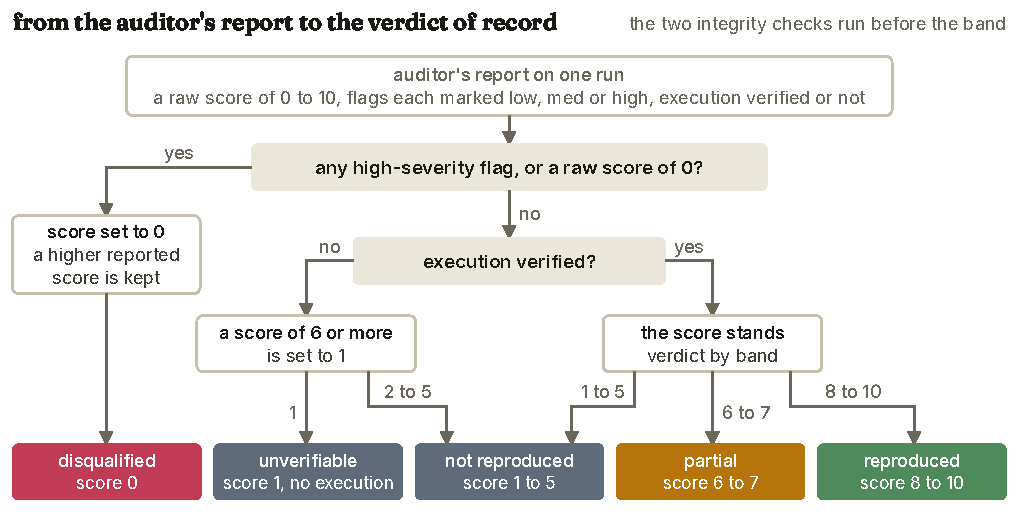
\includegraphics[width=\textwidth]{figures/app_CD_verdict_flow}
\caption{The verdict derivation of the code in Figure~\ref{lst:audit-finalizer}. The integrity checks run
first, and the score then maps to a band, colored as in
Figure~\ref{fig:score-dist}.}
\label{fig:app-cd-verdict-flow}
\end{figure}

\begin{figure}[tb]
\centering
\tcbset{rbFrame/.append style={unbreakable}}
\codefile[lst:audit-finalizer]{Python}{Verdict derivation code}{prompts/audit_finalizer.py}
\end{figure}

% No float barrier here: Table 8 grows with each graded run, and a barrier left three half-empty pages when the two figures above slipped a page. They now print at the top of the next pages.

\section{Auditor Validation}
\label{app:auditor-validation}

We hold four inputs constant across every grade of record: the grader model ID,
which is written onto every verdict row, the frozen rubric file, the audit prompt (Figure~\ref{lst:audit-prompt}) rendered per run from that rubric text and the
pinned claim, and the shared verdict code that applies the integrity adjustment
of Appendix~\ref{app:rubric}. Each grading pass gets an identity of its own from
the grader model name and a UTC timestamp, which keys the audit transcript
the pass writes, so the transcripts of different passes stay
distinguishable. The grading client is given in
Appendix~\ref{app:models}.

Three human graders scored all 396 runs that started, one grader per run, from
the run bundle, its pinned claim, and the rubric text of
Appendix~\ref{app:rubric}, blind to the auditor's score and verdict. Each run
has one human label, so the study measures the auditor against a human grader
and does not measure agreement between humans. The auditor graded 372 of the
396 runs, and Table~\ref{tab:auditor-confusion} compares the two verdicts on
those runs. Taking the human label as the reference, the auditor's reproduced
verdicts reach a precision of 64/73 = 88\% (95\% Wilson interval 78\% to
93\%), a recall of 64/83 = 77\% (67\% to 85\%), and an F1 of 0.82, and the two
agree on the five-way verdict for 306 of the 372 runs. On the 0 to 10 scale
they give the same score to 253 runs and scores within one point to 324, with
a mean absolute difference of 0.59 points and a quadratic weighted kappa of
0.89. The disagreements lean one way. Of
the 28 runs that only one of them called reproduced, the human did in 19 and
the auditor in 9, so the auditor is the stricter grader.
% src: results/e4/summary.json (reproduced_ge8, verdict_agreement 306/372, exact_agreement 253, within_one 324, mae_0_10 0.59, auditor_yes_human_no 9, human_yes_auditor_no 19)

On the 100 runs that either grader placed at 7 or 8, the two agree on 75 about
which side of the reproduced line the run falls, and 18 of the other 25 are
one point apart, with the human at 8 and the auditor at 7 on 11. A score of 0 covers a
high-severity integrity flag and three related conditions
(Table~\ref{tab:rubric}), and of the 57 runs that either grader placed at 0
they agree on 42, with the auditor alone placing 11 there and the human
alone 4. Table~\ref{tab:auditor-tier} gives the reproduced-verdict
agreement by tier. Recall is lowest at Reimplement, where it rests on 16 human
reproductions and its interval of 44\% to 86\% overlaps those of the other
tiers.
% src: results/e4/summary.json (boundary_7_8 100 and 75; disqualified_score0_as_high_severity either 57, both 42; per_tier_reproduced reimplement recall_wilson95 [44.4, 85.8])

\begin{table}[ht]
\centering
\small
\begin{tabular}{@{}lrrrrrr@{}}
\toprule
& \multicolumn{5}{c}{Auditor} & \\
\cmidrule(lr){2-6}
Human & Reproduced & Partial & Not reproduced & Unverifiable & Disqualified & Total \\
\midrule
Reproduced     & 64 & 15 &   2 & 0 &  2 &  83 \\
Partial        &  7 & 64 &  15 & 0 &  2 &  88 \\
Not reproduced &  2 &  6 & 130 & 3 &  5 & 146 \\
Unverifiable   &  0 &  0 &   1 & 6 &  2 &   9 \\
Disqualified   &  0 &  1 &   2 & 1 & 42 &  46 \\
\midrule
Total          & 73 & 86 & 150 & 10 & 53 & 372 \\
\bottomrule
\end{tabular}
\caption{Human verdict against auditor verdict on the 372 runs with both grades.}
\label{tab:auditor-confusion}
\end{table}
% src: results/e4/summary.json verdict_matrix_human_rows; column totals equal auditor_col_totals grouped by band (8-10: 52+16+5 = 73; 6-7: 60+26 = 86; 2-5: 47+17+72+14 = 150; 1: 10; 0: 53)

\begin{table}[ht]
\centering
\small
\begin{tabular}{@{}lrrr@{}}
\toprule
Tier & Precision & Recall & F1 \\
\midrule
Run         & 28/31 = 90\% & 28/35 = 80\% & 0.85 \\
Retrain     & 25/29 = 86\% & 25/32 = 78\% & 0.82 \\
Reimplement & 11/13 = 85\% & 11/16 = 69\% & 0.76 \\
\bottomrule
\end{tabular}
\caption{Agreement of auditor and human on the reproduced verdict, by tier.}
\label{tab:auditor-tier}
\end{table}
% src: results/e4/per_tier.csv (both, auditor_only, human_only); results/e4/summary.json per_tier_reproduced (f1 0.848, 0.82, 0.759)

Table~\ref{tab:auditor-rates} gives the reproduced rate under each grade over
all cells of a tier, with a cell without an auditor grade counted as not
reproduced. The human grade finds more reproductions in every tier and the
tiers keep their order under both. Of the 28 runs that only one grader called
reproduced, the human did in 19 and the auditor in 9, which is 7 against 3 at
Run, 7 against 4 at Retrain, and 5 against 2 at Reimplement.

\begin{table}[ht]
\centering
\small
\begin{tabular}{@{}lrr@{}}
\toprule
Tier & Auditor & Human \\
\midrule
Run         & 31/136 = 23\% (17--31) & 35/136 = 26\% (19--34) \\
Retrain     & 29/132 = 22\% (16--30) & 32/132 = 24\% (18--32) \\
Reimplement & 13/132 = 10\% (6--16)  & 16/132 = 12\% (8--19) \\
\midrule
All tiers   & 73/400 = 18\% (15--22) & 83/400 = 21\% (17--25) \\
\bottomrule
\end{tabular}
\caption{Reproduced cells under the auditor's and the human grade as submitted,
with 95\% Wilson intervals.}
\label{tab:auditor-rates}
\end{table}
% src: results/e4/summary.json per_tier_reproduced (auditor = both + auditor_only, human = both + human_only; run 28 + 3, 28 + 7; retrain 25 + 4, 25 + 7; reimplement 11 + 2, 11 + 5); Wilson recomputed


\section{Dataset Construction Details}
\label{app:construction}

\subsection{Source corpus}
\label{app:corpus}

The corpus starts from the NeurIPS 2025 index of the \emph{ai-conferences}
collection~\citep{neurips2025corpus}, whose entries have matched arXiv IDs; we
keep a row only when that ID is well formed, and we never pair by title. Two
fetch stages pull each paper's arXiv source package and its OpenReview supplement,
matched by forum identifier, into one bundle row per paper with the decoded
\texttt{.tex} text and the supplement files, 3,414 bundled papers, 3,410 with
a \texttt{.tex} file and 1,547 with a supplement.

\subsection{Stage I: artifact-verified classification}
\label{app:classifier}

We sampled 1,000 papers uniformly from the corpus rows with LaTeX source, and
MiniMax-M2.7~\citep{minimax2026m2} classified them.
Each classification runs an agent loop over ten tools, five over GitHub, three
over Hugging Face, a URL fetch, and a supplement reader, and every artifact
signal records how a tool established it. The prompt is
Figure~\ref{lst:classifier-prompt}, where \texttt{\{PAPER\_TEXT\}} stands for
the rendered paper, its supplement manifest with text excerpts, and its LaTeX
source.

\subsection{Deterministic extraction}
\label{app:extraction}

Code computes score and tier from the four signal booleans. Missing code adds
2, missing weights 1, and missing data 3 unless the dataset is a standard
public benchmark; scores of 0, 1, and 2 map to \texttt{Easy} (Run),
\texttt{Medium} (Retrain), and \texttt{Hard} (Reimplement), and 3 stays
\texttt{Hard} when the data are available or standard and is otherwise
\texttt{Artifact-Blocked}, as is any higher score.

\subsection{Stage II: compute capping and stratified selection}
\label{app:selection}

We kept every verified row in the three evaluation tiers with an adjudicated
compute estimate, 620 rows, and took a 200-row pool from them, split equally
across the tiers and spread across the compute bands, cheapest first within
each band. The pool is twice the benchmark size so that the human audit could
drop rows and every tier kept replacements (Table~\ref{tab:audit-pool}). We
applied the 96 H100-hour cap to the evaluation split after the human audit,
replacing three over-cap papers with cheaper same-tier rows from the same
audited pool, so no evaluation paper exceeds the cap although
Table~\ref{tab:audit-pool} still shows pool rows above it. Cheapest-first
changed nothing in four of the twelve tier-by-band strata, whose quotas took
every eligible row, and it selects from the bottom in the eight oversubscribed
ones. The 13 Run-tier rows from the 0 to 8 band are the bottom ninth percentile
of 148 eligible rows, and the 13 Retrain-tier rows from that band all have an
adjudicated estimate of zero hours among 215 eligible rows with a median of
1.0. The band quotas bias the pool in the opposite direction, to a median of
14.78 H100-hours against 3.95 for the eligible set, so the pool favors the
cheapest configurations inside each oversubscribed band and expensive papers
across bands.

\begin{table}[!ht]
\centering
\small
\begin{tabular}{@{}lrrrrrrrr@{}}
\toprule
Tier & Selected & 0--8 & 8--32 & 32--96 & $>$96 & Flagged & Revised & $\Sigma$
H100-h \\
\midrule
Run (\texttt{Easy})          & 67 & 13 & 35 & 14 & 5 & 14 & 6 & 1,961 \\
Retrain (\texttt{Medium})    & 67 & 13 & 39 & 11 & 4 & 22 & 3 & 1,754 \\
Reimplement (\texttt{Hard})  & 66 & 24 & 23 & 11 & 8 & 14 & 4 & 2,190 \\
\midrule
Total & 200 & 50 & 97 & 36 & 17 & 50 & 13 & 5,905 \\
\bottomrule
\end{tabular}
\caption{The 200-paper audit pool by tier and pre-audit H100-hour band, with
rows flagged for compute review, rows the automatic arithmetic check revised,
and summed audited compute.}
\label{tab:audit-pool}
\end{table}

\subsection{Stage III: human audit}
\label{app:human-audit}

For every pool paper we opened the evidence behind each availability call and
recorded a verdict on each of the four signals. A disagreement replaces the model's verdict on that signal, and code recomputes the score and tier from the verdicts. Because a Reimplement-tier assignment rests on no
code having been located, we re-checked those rows with
GPT-5.5~\citep{openai2026gpt55} under web search, and we ran two independent
LLM agents with web search against every claimed wall in that tier, one asking
whether an alternate route to the pinned metric exists inside the paper's
compute band and one re-checking whether the missing-artifact signal still
held. We upheld a wall only when both agents failed to find a route, and two
papers stayed eligible because one agent found one.
Stage III checked the availability calls and the compute estimates. The
claim, the minimal configuration, and the match target of each paper come from
the Stage I classifier, and an author reviewed each of these fields before the
freeze with no second reviewer, so we report no annotator agreement for them.
Appendix~\ref{app:target-check} checks each frozen target against its paper.

\subsection{Target check}
\label{app:target-check}

We checked every frozen target against its paper with gpt-6.1-sol~\citep{openai2026gpt61sol},
a model from a different lab than the auditor. Given the paper text, the
claim sentence, and the frozen metric, dataset and split, configuration, and
value, it answered four yes-or-no questions with a supporting quotation each,
whether the paper reports this value within rounding, for this metric, on this
dataset and split, and for this method or variant. Implementation details of
the released code, such as checkpoint names, step counts, seeds, and hardware,
were out of scope. Because the model saw the frozen target, this checks each
target against its paper and does not re-derive it. The value and metric
questions check the target, the dataset and method questions check the
minimal configuration, and the choice of claim rests on the author review alone.
Table~\ref{tab:target-check} gives the counts.
% src: results/e7/README.md:3-5 (gpt-6.1-sol, reasoning high, pdftotext of the arXiv PDF; four questions; out-of-scope details)

\begin{table}[ht]
\centering
\small
\begin{tabular}{@{}lrrrrr@{}}
\toprule
The paper supports the frozen & Of 100 & 95\% interval & Run & Retrain & Reimplement \\
\midrule
Value          & 92 & 85--96 & 32/34 & 29/33 & 31/33 \\
Metric         & 95 & 89--98 & 32/34 & 30/33 & 33/33 \\
Dataset and split & 76 & 67--83 & 24/34 & 25/33 & 27/33 \\
Method or variant & 69 & 59--77 & 22/34 & 18/33 & 29/33 \\
\midrule
All four       & 55 & 45--64 & 19/34 & 13/33 & 23/33 \\
\bottomrule
\end{tabular}
\caption{Frozen targets whose paper supports each part, by tier.}
\label{tab:target-check}
\end{table}
% src: results/e7/summary.json step3 (by_question yes and wilson95; by_tier Easy/Medium/Hard a-d; all_four_yes 55, wilson95 [0.4524, 0.6439]); all-four by tier counted from results/e7/step3.jsonl (a to d all yes: Easy 19, Medium 13, Hard 23)

The most common failure is the method question alone, on 18 papers. On
2506.18890, for example, the frozen value of 27.443 PSNR appears in the paper
for 24 input views, while the frozen configuration says 12.
% src: results/e7/README.md:9-10; results/e7/v3_failures.csv

Of the 100 targets, 55 pass all four questions. A second check flags a target
only where the paper contradicts it, and it sorted the other 45 as follows: the
frozen number is wrong on 8, the number is right but a setting or label is off
on 16, and the target is correct or the paper is ambiguous on 21. We corrected
the 8 numbers to the paper's value and rescored their runs, which changes two
verdicts, both on 2505.23747. Its frozen value of 51.13 comes from the
authors' README, while the paper, which defines the claim, reports 48.4, and
DeepSeek-V4-Flash (51.44 measured) and MiniMax-M2.7 move from reproduced to
partial. DeepSeek-V4-Flash then reproduces 13 of 34 Run papers where the
submission reported 14.
% src: rebuttal/mithil/e7_merged.md (Kind of error column: number 8, setting or label 15 + 1, none 21); results/e7/rescore_summary.md and class_d_rescore.md (two verdicts, 14 to 13); results/e7/summary.json step3 (all_four_yes 55)

\subsection{The evaluation and development splits}
\label{app:splits}

We applied the human verdicts, recomputed each paper's score and tier, and
dropped any paper whose minimal experiment calls a paid or closed model API.
The Stage II rule then selected the evaluation split from what remained, the
development split took the cheapest eligible papers left in each tier, and
Appendix~\ref{app:dataset-schema} gives their sizes.
Figure~\ref{fig:app-ef-compute-strip} shows the audited compute of the 100
evaluation papers by tier, and Figure~\ref{fig:app-ef-arxiv-months} shows
their arXiv posting months.

\begin{figure}[htb]
\centering
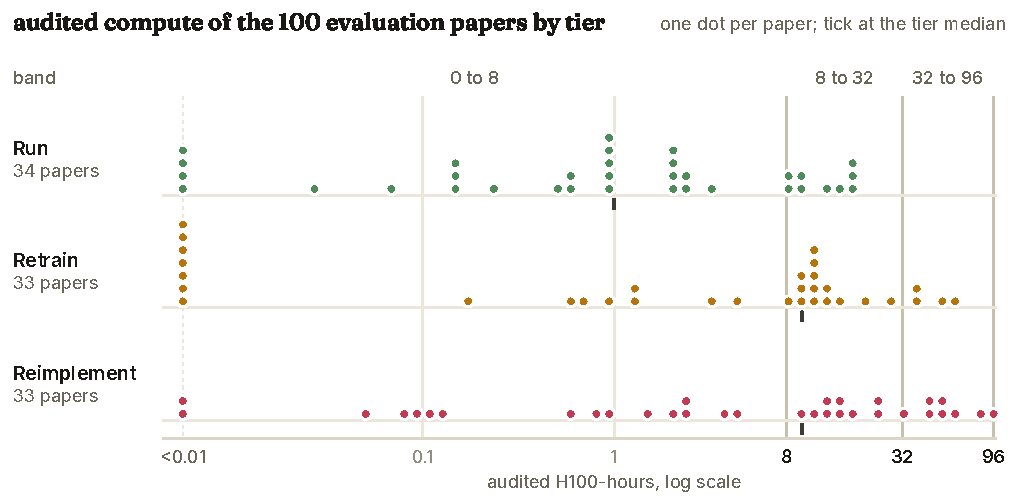
\includegraphics[width=\textwidth]{figures/app_EF_compute_strip}
\caption{The audited compute of the 100 evaluation papers, one dot per paper
on a log axis, with a tick at each tier's median and papers below the axis
floor in the leftmost slot.}
\label{fig:app-ef-compute-strip}
\end{figure}

\begin{figure}[htb]
\centering
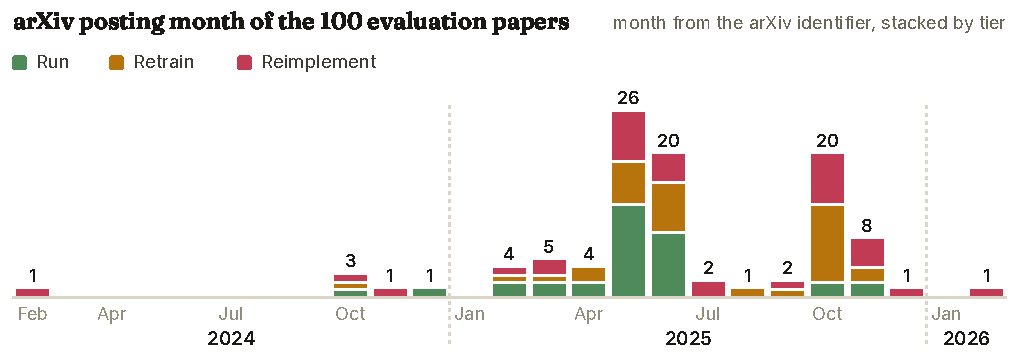
\includegraphics[width=\textwidth]{figures/app_EF_arxiv_months}
\caption{The 100 evaluation papers by the month of their arXiv identifier,
stacked by tier.}
\label{fig:app-ef-arxiv-months}
\end{figure}

\clearpage  % Appendix F opens a page, so the field table and the example row print beside their citation
\section{Dataset Fields}
\label{app:dataset-schema}

We release the audited benchmark after review as a \texttt{datasets}
dataset~\citep{lhoest2021datasets} with two splits and no \texttt{train}
split. The \texttt{test} split, marked \texttt{split="eval"}, is the 100-paper
frozen benchmark, and the \texttt{validation} split, marked \texttt{split="dev"},
is the 14-paper development set (Table~\ref{tab:splits}), and no arXiv ID
appears in both. Every row holds the 25 top-level fields and four nested objects of
Table~\ref{tab:schema}, fixed before any agent starts. Figure~\ref{lst:example-row} shows the SharpZO row of
Section~\ref{subsec:task} (availability score 0, Run tier, 0.07 H100-hours, band
\texttt{0-8}), long text fields truncated and the rest verbatim. Rows return
metadata and links only, with no full paper text.

\begin{table}[ht]
\centering
\small
\begin{tabular}{@{}lrrrrrr@{}}
\toprule
& \multicolumn{5}{c}{Evaluation split} & Development split \\
\cmidrule(lr){2-6} \cmidrule(lr){7-7}
Tier & Papers & 0--8 & 8--32 & 32--96 & Audited H100-h & Papers \\
\midrule
Run         & 34  & 27 & 7  & 0  & 142.71    & 5  \\
Retrain     & 33  & 16 & 13 & 4  & 380.91    & 4  \\
Reimplement & 33  & 16 & 9  & 8  & 630.18    & 5  \\
\midrule
All         & 100 & 59 & 29 & 12 & 1{,}153.8 & 14 \\
\bottomrule
\end{tabular}
\caption{Composition of the two splits by tier and compute band, with papers
binned by the audited H100-hour estimate.}
\label{tab:splits}
\end{table}

{\footnotesize
\begin{longtable}{@{}>{\raggedright\arraybackslash}p{4.95cm}>{\raggedright\arraybackslash}p{1.95cm}>{\raggedright\arraybackslash}p{5.65cm}@{}}
\toprule
Field & Type & Description \\
\midrule
\endfirsthead
\multicolumn{3}{@{}l}{\footnotesize\itshape Table~\ref{tab:schema}, continued.} \\[3pt]
\toprule
Field & Type & Description \\
\midrule
\endhead
\midrule
\endfoot
\bottomrule
\noalign{\vskip 6pt}
\caption{The fields of a dataset row.}
\label{tab:schema} \\
\endlastfoot
\multicolumn{3}{@{}>{\raggedright\arraybackslash}p{13.4cm}@{}}{\emph{Top-level fields}} \\
\texttt{custom\_id} & string & arXiv ID, the primary key. \\
\texttt{central\_claim} & string & The paper's central empirical claim in one sentence. \\
\texttt{claim\_evidence} & string & Quoted paper text grounding the claim. \\
\texttt{mre\_config} & string & Prose recipe for the cheapest configuration that tests the claim, withheld from the agent. \\
\texttt{agent\_task} & string & Classifier-written reproduction instruction, released with the row and shown to neither the agent nor the auditor. \\
\texttt{verified\_links} & object & Tool-confirmed artifact URLs. \\
\texttt{signals} & object & Per-artifact availability audit. \\
\texttt{match\_target} & object & The quantity a run must match. \\
\texttt{h100\_estimate} & object & Compute estimate and its basis. \\
\texttt{score} & int & Artifact-availability score from the four signals; shipped rows take 0 to 3. \\
\texttt{tier} & string & \texttt{Easy}, \texttt{Medium} or \texttt{Hard} in the released dataset, for the Run, Retrain and Reimplement tiers; derived from \texttt{score}. \\
\texttt{split} & string & \texttt{eval} (test split) or \texttt{dev} (validation split). \\
\texttt{selection\_band} & string & Compute band used for stratified selection. \\
\texttt{h100\_band} & string & Compute band, one of \texttt{0-8}, \texttt{8-32}, \texttt{32-96}. \\
\texttt{h100\_hours\_estimate} & float & Estimated H100-hours to run the match target. \\
\texttt{h100\_estimate\_basis} & string & Free-text justification for the estimate. \\
\texttt{audited\_h100\_hours} & float & Recomputed product where the arithmetic audit flagged the stated hours and the selection code accepted it, otherwise the stated estimate (Appendix~\ref{app:selection}). \\
\texttt{h100\_recomputed\_hours} & float or null & Hours recomputed from the estimate's arithmetic; null when an input is missing. \\
\texttt{h100\_arithmetic\_mismatch} & bool or null & Flag set when estimate arithmetic disagreed. \\
\texttt{h100\_hours\_adjudicated} & bool & Whether the recompute replaced the stated estimate. \\
\texttt{h100\_needs\_human\_review} & bool & Whether the estimate was flagged for review. \\
\texttt{paper\_kind} & string & Paper type. All rows are \texttt{empirical}. \\
\texttt{verification\_status} & string & Classifier verification state. All rows are \texttt{verified}. \\
\texttt{web\_verification} & string & Web-retrieval state. All rows are \texttt{available}. \\
\texttt{exit\_reason} & string & Classifier exit reason. All rows are \texttt{natural}. \\
\addlinespace
\multicolumn{3}{@{}>{\raggedright\arraybackslash}p{13.4cm}@{}}{\emph{\texttt{verified\_links} (lists of tool-confirmed URLs, empty when none located)}} \\
\texttt{paper\_or\_project} & list of strings & Paper or project-page URLs. \\
\texttt{code} & list of strings & Code repository URLs. \\
\texttt{dataset} & list of strings & Dataset URLs. \\
\texttt{weights} & list of strings & Model-weight URLs. \\
\addlinespace
\multicolumn{3}{@{}>{\raggedright\arraybackslash}p{13.4cm}@{}}{\emph{\texttt{signals} (one object per audited signal: \texttt{code\_available}, \texttt{dataset\_available}, \texttt{weights\_available}, \texttt{dataset\_is\_standard})}} \\*
\texttt{value} & bool & Whether the artifact is present. \\
\texttt{verification} & string & \texttt{tool\_verified}, \texttt{tool\_searched\_not\_found} or \texttt{not\_applicable}. \\
\texttt{evidence} & string & The tool observation supporting the value. \\
\addlinespace
\multicolumn{3}{@{}>{\raggedright\arraybackslash}p{13.4cm}@{}}{\emph{\texttt{match\_target} (the quantity a run must recover to count as a match)}} \\
\texttt{config} & string & Experimental configuration that produces the target value. \\
\texttt{metric} & string & The reported metric name. \\
\texttt{value} & string & The target value to match. \\
\texttt{scope} & string & The model, dataset or setting the value applies to. \\
\texttt{match\_bar\_kind} & string & \texttt{point\_estimate}, \texttt{direction}, \texttt{threshold}, \texttt{magnitude} or \texttt{range}. \\
\addlinespace
\multicolumn{3}{@{}>{\raggedright\arraybackslash}p{13.4cm}@{}}{\emph{\texttt{h100\_estimate} (the compute estimate that placed the paper in its band)}} \\
\texttt{hours} & float & Estimated H100-hours for the match target. \\
\texttt{basis\_kind} & string & \texttt{derived\_from\_config}, \texttt{paper\_reported}, \texttt{comparable\_experiment} or \texttt{compute\_unspecified}. \\
\texttt{gpu\_count} & int or null & GPU count the paper reports. \\
\texttt{gpu\_type} & string or null & GPU type the paper reports. \\
\texttt{wallclock\_hours} & float or null & Reported wall-clock hours, before H100 normalization. \\
\texttt{h100\_equivalent\_multiplier} & float or null & Factor converting the reported GPU to H100-equivalent hours. \\
\texttt{basis} & string & Free-text justification for the estimate. \\
\end{longtable}
}

\codefile[lst:example-row]{json}{One evaluation row (2506.20990)}{prompts/example_row.json}

\paragraph{Match targets and tolerance.} For 62 of the 100 evaluation papers
the match bar is a point estimate, for 21 a stated baseline the run must beat,
for 14 a reported threshold it must clear, for 1 the size of a reported delta,
and for 1 a reported range it must fall inside. A run matches a
point estimate when its measured value lies within the authors' stated
tolerance, or within 5\% relative when the paper states none
(Figure~\ref{lst:rubric-text}), and 58 of the 62 point estimates use the 5\%
default. To measure how much the default decides, we rescored every graded run
at relative tolerances of 1\%, 2\%, and 10\% (Table~\ref{tab:tolerance}). The
ordering of the tiers holds at every setting, and the best agent's count moves
by at most 5 papers at Run, 3 at Retrain, and 1 at Reimplement. Tightening to
1\% moves 17 of the 73 reproduced runs to partial, and loosening to 10\% moves
up 9 partial runs whose only failed criterion was the number. For example,
DeepSeek-V4-Flash measured 90.6 on 2511.19808 against a frozen target of 97.3,
a gap of $6.7 / 97.3 = 6.9\%$, so that run is partial at 5\% and reproduced at
10\%. With an absolute tolerance of 1 or 2 points on percentage metrics, 70 or
72 of the 400 cells reproduce.
% src: results/e6/summary.json (claims: 62 point estimates, point_estimate_default_5pct 58, point_estimate_stated_margin 4; falls_by_setting rel1 17; number_only_partials 9; settings abs1, abs2); results/e6/README.md:13-24 (worked run; best-agent table)

\begin{table}[ht]
\centering
\small
\begin{tabular}{@{}lrrrr@{}}
\toprule
Relative tolerance & Run, best of 34 & Retrain, best of 33 & Reimplement, best of 33 & All agents, of 400 \\
\midrule
1\%           &  9 &  8 & 4 & 56 \\
2\%           & 12 &  9 & 5 & 65 \\
5\% (default) & 14 &  9 & 5 & 73 \\
10\%          & 14 & 12 & 5 & 82 \\
\bottomrule
\end{tabular}
\caption{Reproduced cells at four relative tolerances, for the best agent in
each tier and over all agents.}
\label{tab:tolerance}
\end{table}
% src: results/e6/README.md:19-24 (best agent per tier); results/e6/summary.json cells summed per setting (56, 65, 73, 82)
% moves with: E7 and the regrade decision (the 5% row becomes the post-correction counts); rerun rel1/rel2/rel10 if the counts of record change

\newpage  % this paragraph opens a page, so both paper tables print within a page of it
\paragraph{The evaluation and development papers.} Tables~\ref{tab:eval100}
and~\ref{tab:dev14} list the 100 evaluation and 14 development papers with the
match target each is graded against, where Band is the compute band in
H100-hours, H100-h the audited estimate for that paper's match target, and Metric, Bar,
and Target value the pinned match target, with Bar written unset on the one
evaluation row with no bar kind. The
development split totals 26.89 audited H100-hours.

% Generated by paper_latex/tables/gen_eval100.py. Do not edit by hand.
% src: outputs/v6/app_rebuild/eval_100.jsonl
{\scriptsize
\begin{longtable}{@{}l@{\hspace{4pt}}l@{\hspace{4pt}}>{\centering\arraybackslash}p{0.9cm}@{\hspace{4pt}}>{\raggedleft\arraybackslash}p{1.1cm}@{\hspace{8pt}}p{3.2cm}@{\hspace{5pt}}p{1.6cm}@{\hspace{5pt}}p{3.3cm}@{}}
\toprule
arXiv & Tier & Band & H100-h & Metric & Bar & Target value \\
\midrule
\endfirsthead
\multicolumn{7}{@{}l}{\footnotesize\itshape Table~\ref{tab:eval100}, continued.} \\[3pt]
\toprule
arXiv & Tier & Band & H100-h & Metric & Bar & Target value \\
\midrule
\endhead
\midrule
\endfoot
\bottomrule
\noalign{\vskip 6pt}
\caption{The 100 evaluation papers, one row each, sorted by tier, then compute band, then arXiv ID. Metric names and target values longer than 28 characters are cut and closed with an ellipsis.}
\label{tab:eval100} \\
\endlastfoot
2502.05795 & Run & 0--8 & 1.00 & \raggedright Validation perplexity... & \raggedright point estimate & \raggedright 25.76 \tabularnewline
2502.06684 & Run & 0--8 & $<$0.01 & \raggedright Mean accuracy (\%) on 10... & \raggedright point estimate & \raggedright 77.0 +/- 1.8\% \tabularnewline
2503.18430 & Run & 0--8 & 0.64 & \raggedright Average Precision (AP) & \raggedright point estimate & \raggedright 46.3\% \tabularnewline
2503.23035 & Run & 0--8 & 0.25 & \raggedright PSNR (dB) & \raggedright point estimate & \raggedright 27.69 \tabularnewline
2504.20571 & Run & 0--8 & 0.16 & \raggedright MATH500 accuracy (\%) & \raggedright point estimate & \raggedright 73.6\% \tabularnewline
2505.10978 & Run & 0--8 & 2.00 & \raggedright Success rate (\%) & \raggedright point estimate & \raggedright 86.7\% \tabularnewline
2505.11483 & Run & 0--8 & 0.00 & \raggedright Peak RAM usage & \raggedright point estimate & \raggedright 8.56 kB \tabularnewline
2505.14766 & Run & 0--8 & 1.00 & \raggedright Mean Absolute Scaled Error... & \raggedright point estimate & \raggedright 0.617 \tabularnewline
2505.14827 & Run & 0--8 & 8.00 & \raggedright Accuracy (\%) & \raggedright direction & \raggedright 59.53\% \tabularnewline
2505.18456 & Run & 0--8 & 2.50 & \raggedright test perplexity (PPL, lower... & \raggedright point estimate & \raggedright 21.66 \tabularnewline
2505.18809 & Run & 0--8 & 2.00 & \raggedright end-to-end video generation... & \raggedright point estimate & \raggedright 1.76x \tabularnewline
2505.19154 & Run & 0--8 & 0.03 & \raggedright PSNR (dB) on rendered novel... & \raggedright point estimate & \raggedright 30.9 \tabularnewline
2505.19713 & Run & 0--8 & 0.64 & \raggedright Mean Chamfer Distance ($\times$10$^3$) & \raggedright point estimate & \raggedright 6.54 \tabularnewline
2505.23747 & Run & 0--8 & 2.56 & \raggedright VSI-Bench micro average... & \raggedright point estimate & \raggedright 51.13\% \tabularnewline
2505.24864 & Run & 0--8 & 8.00 & \raggedright Average pass@1 improvement... & \raggedright direction & \raggedright 15.7\% \tabularnewline
2505.24873 & Run & 0--8 & 1.00 & \raggedright SSIM (structural similarity) & \raggedright point estimate & \raggedright 0.9842 \tabularnewline
2506.02392 & Run & 0--8 & $<$0.01 & \raggedright optimality gap (\%) & \raggedright point estimate & \raggedright 3.25\% \tabularnewline
2506.10351 & Run & 0--8 & 1.00 & \raggedright Classification accuracy (\%) & \raggedright point estimate & \raggedright 93.12\% \tabularnewline
2506.12025 & Run & 0--8 & 0.50 & \raggedright Prediction speedup... & \raggedright direction & \raggedright 100x \tabularnewline
2506.18890 & Run & 0--8 & $<$0.01 & \raggedright PSNR (dB) & \raggedright point estimate & \raggedright 27.443 \tabularnewline
2506.20671 & Run & 0--8 & 0.16 & \raggedright PQ-All (\%) & \raggedright point estimate & \raggedright 6.30 \tabularnewline
2506.20990 & Run & 0--8 & 0.07 & \raggedright test accuracy (\%) & \raggedright point estimate & \raggedright 79.42\% \tabularnewline
2506.21724 & Run & 0--8 & 2.00 & \raggedright Overall accuracy (\%) on... & \raggedright point estimate & \raggedright 90.53\% \tabularnewline
2510.21311 & Run & 0--8 & 0.16 & \raggedright gIoU (generic Intersection... & \raggedright point estimate & \raggedright 55.1 \tabularnewline
2510.23574 & Run & 0--8 & 3.00 & \raggedright absolute relative error... & \raggedright threshold & \raggedright 7.5 \tabularnewline
2511.00090 & Run & 0--8 & 1.00 & \raggedright Latency speedup ratio & \raggedright point estimate & \raggedright 2.59x \tabularnewline
2511.16666 & Run & 0--8 & 2.00 & \raggedright Orientation accuracy at... & \raggedright point estimate & \raggedright 89.47\% \tabularnewline
2410.18164 & Run & 8--32 & 18.00 & \raggedright CC18 AUC / CTR23 R2 & \raggedright threshold & \raggedright AUC \textgreater{}= 0.92 (paper 0.933)... \tabularnewline
2412.11979 & Run & 8--32 & 16.00 & \raggedright Zipf power-law exponent... & \raggedright range & \raggedright approx 0.8-1.0 (observed... \tabularnewline
2504.12397 & Run & 8--32 & 10.00 & \raggedright Classification accuracy (\%) & \raggedright direction & \raggedright 79.30\% (LoRA) vs 81.94\%... \tabularnewline
2505.10475 & Run & 8--32 & 18.00 & \raggedright GSM8K accuracy... & \raggedright unset & \raggedright ParScale-1.8B-P8 approx... \tabularnewline
2505.23305 & Run & 8--32 & 10.24 & \raggedright FAD (Fr\'echet Audio... & \raggedright point estimate & \raggedright 0.47 \tabularnewline
2506.01511 & Run & 8--32 & 18.00 & \raggedright Black-box attack success... & \raggedright threshold & \raggedright \textgreater{}50\% black-box ASR (paper... \tabularnewline
2506.18896 & Run & 8--32 & 12.80 & \raggedright MATH500 accuracy & \raggedright threshold & \raggedright \textgreater{}80\% (vs \textasciitilde{}73\%... \tabularnewline
2502.01203 & Retrain & 0--8 & 0.96 & \raggedright Win rate against preferred... & \raggedright direction & \raggedright 66.1\% \tabularnewline
2503.09657 & Retrain & 0--8 & 4.16 & \raggedright Wikitext2 perplexity (lower... & \raggedright threshold & \raggedright 16.17 \tabularnewline
2504.13146 & Retrain & 0--8 & 8.00 & \raggedright distilled student accuracy... & \raggedright point estimate & \raggedright \textasciitilde{}40\% \tabularnewline
2505.15201 & Retrain & 0--8 & 0.00 & \raggedright empirical variance of... & \raggedright magnitude & \raggedright \textasciitilde{}10x lower variance than... \tabularnewline
2505.17836 & Retrain & 0--8 & 0.00 & \raggedright Average normalized absolute... & \raggedright point estimate & \raggedright \textasciitilde{}0.05 \tabularnewline
2505.21077 & Retrain & 0--8 & 1.28 & \raggedright throughput speedup & \raggedright point estimate & \raggedright 1.20x \tabularnewline
2505.24680 & Retrain & 0--8 & 1.28 & \raggedright Average perplexity on... & \raggedright point estimate & \raggedright 24.59 \tabularnewline
2506.06991 & Retrain & 0--8 & 0.00 & \raggedright Area Under ROC Curve (AUC) & \raggedright point estimate & \raggedright 0.91 \tabularnewline
2506.07673 & Retrain & 0--8 & 0.00 & \raggedright estimation gap reduction vs... & \raggedright point estimate & \raggedright 37.2\% \tabularnewline
2506.20233 & Retrain & 0--8 & 0.00 & \raggedright Recovery accuracy... & \raggedright point estimate & \raggedright negligible bias and... \tabularnewline
2509.16391 & Retrain & 0--8 & 0.67 & \raggedright Average Gap (lower is... & \raggedright direction & \raggedright 0.25 \tabularnewline
2510.07501 & Retrain & 0--8 & 0.00 & \raggedright Bias of MR estimator value... & \raggedright point estimate & \raggedright -0.20 \tabularnewline
2510.09485 & Retrain & 0--8 & 0.00 & \raggedright Worst-case total variation... & \raggedright direction & \raggedright Local sampler TV \textless{} Global... \tabularnewline
2510.20725 & Retrain & 0--8 & 3.12 & \raggedright cumulative regret growth... & \raggedright direction & \raggedright sublinear (grows slower... \tabularnewline
2510.21363 & Retrain & 0--8 & 0.17 & \raggedright gender fairness score (0-1... & \raggedright point estimate & \raggedright 0.560 \tabularnewline
2510.23577 & Retrain & 0--8 & 0.64 & \raggedright Average Precision (AP) in... & \raggedright point estimate & \raggedright 98.89 \tabularnewline
2410.19933 & Retrain & 8--32 & 13.00 & \raggedright safety rate (fraction of... & \raggedright threshold & \raggedright \textgreater{}90\% safety rate, above the... \tabularnewline
2505.24089 & Retrain & 8--32 & 12.80 & \raggedright membership-inference AUC on... & \raggedright point estimate & \raggedright \textasciitilde{}82.45\% AUC (paper Table 1... \tabularnewline
2506.08898 & Retrain & 8--32 & 9.60 & \raggedright Normalized Hypervolume (HV) & \raggedright direction & \raggedright 0.6411 \tabularnewline
2506.10943 & Retrain & 8--32 & 12.00 & \raggedright no-context SQuAD QA... & \raggedright direction & \raggedright paper full-scale: base... \tabularnewline
2506.13717 & Retrain & 8--32 & 9.60 & \raggedright Top-1 classification... & \raggedright point estimate & \raggedright 90.21\% \tabularnewline
2510.05874 & Retrain & 8--32 & 15.36 & \raggedright Full Rollout MSE & \raggedright point estimate & \raggedright 1.259e-6 \tabularnewline
2510.10480 & Retrain & 8--32 & 29.44 & \raggedright ISM (Interaction Site... & \raggedright point estimate & \raggedright 52.15\% \tabularnewline
2510.19314 & Retrain & 8--32 & 10.24 & \raggedright Average performance (PERF.) & \raggedright point estimate & \raggedright 0.7923 \tabularnewline
2510.19784 & Retrain & 8--32 & 12.00 & \raggedright test MSE on LV trajectory... & \raggedright threshold & \raggedright paper reports 7.93e-5; bar... \tabularnewline
2510.22123 & Retrain & 8--32 & 10.96 & \raggedright Force MAE (kcal/mol/\AA{}) & \raggedright point estimate & \raggedright 0.102 \tabularnewline
2510.24940 & Retrain & 8--32 & 12.00 & \raggedright answer accuracy on SVAMP... & \raggedright point estimate & \raggedright \textasciitilde{}46\% (paper Table 1... \tabularnewline
2511.00119 & Retrain & 8--32 & 12.00 & \raggedright FID of generated... & \raggedright direction & \raggedright Rectified Flow FID clearly... \tabularnewline
2511.02652 & Retrain & 8--32 & 20.80 & \raggedright SSIM reconstruction quality & \raggedright point estimate & \raggedright 0.8541 \tabularnewline
2504.12463 & Retrain & 32--96 & 35.84 & \raggedright validation perplexity & \raggedright direction & \raggedright 23.48 \tabularnewline
2505.02391 & Retrain & 32--96 & 60.00 & \raggedright Average @ 8 accuracy on... & \raggedright direction & \raggedright \textasciitilde{}71-73\% (vs RAFT++ baseline... \tabularnewline
2506.19839 & Retrain & 32--96 & 48.89 & \raggedright FID 10K & \raggedright point estimate & \raggedright 29.56 \tabularnewline
2508.21046 & Retrain & 32--96 & 36.10 & \raggedright Task success rate & \raggedright point estimate & \raggedright 98.6\% \tabularnewline
2402.04579 & Reimplement & 0--8 & 0.00 & \raggedright Combined cost (modification... & \raggedright direction & \raggedright CCE achieves best combined... \tabularnewline
2410.15392 & Reimplement & 0--8 & 2.00 & \raggedright PSNR (novel view synthesis)... & \raggedright direction & \raggedright up to 3dB higher PSNR and... \tabularnewline
2503.02809 & Reimplement & 0--8 & 0.00 & \raggedright Sharpness S(theta)... & \raggedright point estimate & \raggedright Sharpness oscillates around... \tabularnewline
2505.12677 & Reimplement & 0--8 & 0.60 & \raggedright LPIPS\_e (erasure LPIPS)... & \raggedright threshold & \raggedright 0.41 (Table 1, Kelly... \tabularnewline
2505.19087 & Reimplement & 0--8 & 0.08 & \raggedright Generalization bound value... & \raggedright threshold & \raggedright 0.60302 \tabularnewline
2505.22860 & Reimplement & 0--8 & 1.00 & \raggedright DDI AUC-ROC & \raggedright threshold & \raggedright 0.99 \tabularnewline
2505.24452 & Reimplement & 0--8 & 0.86 & \raggedright validation accuracy (\%) & \raggedright point estimate & \raggedright 94.57$\pm$0.33 \tabularnewline
2506.17475 & Reimplement & 0--8 & 0.10 & \raggedright Test accuracy & \raggedright point estimate & \raggedright 79.01\% \tabularnewline
2507.06489 & Reimplement & 0--8 & 2.56 & \raggedright \% affected samples with... & \raggedright threshold & \raggedright 7.0\% \tabularnewline
2509.16950 & Reimplement & 0--8 & 1.60 & \raggedright Poisoned MVR (mission... & \raggedright point estimate & \raggedright 1.00 \tabularnewline
2510.05767 & Reimplement & 0--8 & 4.60 & \raggedright convergence speed =... & \raggedright direction & \raggedright Greedy-64 converges faster... \tabularnewline
2510.08177 & Reimplement & 0--8 & 0.11 & \raggedright Top-1 accuracy (\%) & \raggedright point estimate & \raggedright 65.9\% \tabularnewline
2510.25146 & Reimplement & 0--8 & 0.05 & \raggedright PSNR (peak signal-to-noise... & \raggedright point estimate & \raggedright 25.8 \tabularnewline
2511.20906 & Reimplement & 0--8 & 2.22 & \raggedright task success rate & \raggedright threshold & \raggedright 100\% \tabularnewline
2512.02339 & Reimplement & 0--8 & 0.12 & \raggedright J\&F mean (Jaccard +... & \raggedright point estimate & \raggedright 77.6\% \tabularnewline
2602.03066 & Reimplement & 0--8 & 4.00 & \raggedright NTK availability A(K,g) =... & \raggedright direction & \raggedright availability(shortcut) \textgreater{}... \tabularnewline
2411.06890 & Reimplement & 8--32 & 23.04 & \raggedright Structural Hamming Distance... & \raggedright direction & \raggedright 1.51 \tabularnewline
2502.08924 & Reimplement & 8--32 & 12.00 & \raggedright test accuracy (greedy... & \raggedright point estimate & \raggedright 0.456 \tabularnewline
2505.10039 & Reimplement & 8--32 & 24.00 & \raggedright circuit completeness =... & \raggedright direction & \raggedright Ns+Dn yields higher... \tabularnewline
2505.16927 & Reimplement & 8--32 & 9.60 & \raggedright IFEval principle-following... & \raggedright threshold & \raggedright 65.6\% \tabularnewline
2506.00070 & Reimplement & 8--32 & 15.36 & \raggedright Spatial reasoning score... & \raggedright point estimate & \raggedright 1.51 \tabularnewline
2507.02064 & Reimplement & 8--32 & 16.00 & \raggedright L2 distance from decoded... & \raggedright point estimate & \raggedright \textasciitilde{}0 cm after convergence... \tabularnewline
2510.25529 & Reimplement & 8--32 & 13.48 & \raggedright Total Average Return (TAR) & \raggedright point estimate & \raggedright 891.7$\pm$19.1 \tabularnewline
2511.01463 & Reimplement & 8--32 & 12.80 & \raggedright R precision Top-3 & \raggedright point estimate & \raggedright 0.785 \tabularnewline
2511.02225 & Reimplement & 8--32 & 18.00 & \raggedright policy learning success rate & \raggedright point estimate & \raggedright 0.95$\pm$0.03 \tabularnewline
2503.14698 & Reimplement & 32--96 & 78.08 & \raggedright PSNR (dB) & \raggedright threshold & \raggedright 30.61 \tabularnewline
2505.22596 & Reimplement & 32--96 & 64.00 & \raggedright gIoU on ReasonSeg zero-shot... & \raggedright point estimate & \raggedright 60.2\% \tabularnewline
2506.02882 & Reimplement & 32--96 & 43.52 & \raggedright Intersection over Union... & \raggedright point estimate & \raggedright 77.0\% \tabularnewline
2506.20024 & Reimplement & 32--96 & 47.36 & \raggedright CRPS (mean across... & \raggedright point estimate & \raggedright 0.904$\times$10$^{-2}$ (0.00904) \tabularnewline
2510.04136 & Reimplement & 32--96 & 56.00 & \raggedright exact & \raggedright direction & \raggedright exact \tabularnewline
2510.15194 & Reimplement & 32--96 & 48.64 & \raggedright Downstream classification... & \raggedright direction & \raggedright 89.68 \tabularnewline
2510.23429 & Reimplement & 32--96 & 96.00 & \raggedright Median Chamfer Distance... & \raggedright point estimate & \raggedright 0.20 \tabularnewline
2511.19808 & Reimplement & 32--96 & 32.40 & \raggedright Test accuracy (\%) & \raggedright point estimate & \raggedright 97.3 \tabularnewline
\end{longtable}
}

% src: outputs/v6/app_rebuild/dev_split.jsonl
{\scriptsize
\begin{longtable}{@{}l@{\hspace{4pt}}l@{\hspace{4pt}}>{\centering\arraybackslash}p{0.9cm}@{\hspace{4pt}}>{\raggedleft\arraybackslash}p{1.1cm}@{\hspace{8pt}}p{3.2cm}@{\hspace{5pt}}p{1.6cm}@{\hspace{5pt}}p{3.3cm}@{}}
\toprule
arXiv & Tier & Band & H100-h & Metric & Bar & Target value \\
\midrule
\endfirsthead
\multicolumn{7}{@{}l}{\footnotesize\itshape Table~\ref{tab:dev14}, continued.} \\[3pt]
\toprule
arXiv & Tier & Band & H100-h & Metric & Bar & Target value \\
\midrule
\endhead
\midrule
\endfoot
\bottomrule
\noalign{\vskip 6pt}
\caption{The 14 development papers, in the same columns, sort order, and truncation as Table~\ref{tab:eval100}. This split is disjoint from the evaluation set and is used for harness development only.}
\label{tab:dev14} \\
\endlastfoot
2505.18513 & Run & 0--8 & 0.01 & \raggedright LDS (Linear Datamodeling... & \raggedright point estimate & \raggedright 21.11 \tabularnewline
2506.09045 & Run & 0--8 & $<$0.01 & \raggedright end-to-end latency speedup & \raggedright point estimate & \raggedright 2.68x \tabularnewline
2507.02546 & Run & 0--8 & 0.01 & \raggedright Metric point map relative... & \raggedright threshold & \raggedright 4.44\% \tabularnewline
2510.21323 & Run & 0--8 & 0.01 & \raggedright Unified concept extraction... & \raggedright point estimate & \raggedright Unified concept set shared... \tabularnewline
2511.07099 & Run & 0--8 & 0.01 & \raggedright Speaker similarity score... & \raggedright point estimate & \raggedright 0.113 \tabularnewline
2502.06067 & Retrain & 0--8 & 2.00 & \raggedright 95\% CI coverage rate & \raggedright threshold & \raggedright 1.0 (100\%) \tabularnewline
2502.08101 & Retrain & 0--8 & 1.00 & \raggedright Mean accuracy (\%) & \raggedright point estimate & \raggedright 94.98\% \tabularnewline
2505.19458 & Retrain & 0--8 & 2.50 & \raggedright Sudoku board accuracy on... & \raggedright point estimate & \raggedright 34.4\% \tabularnewline
2505.13431 & Retrain & 8--32 & 12.00 & \raggedright Success rate (\%) & \raggedright point estimate & \raggedright 98.0\% \tabularnewline
2505.17282 & Reimplement & 0--8 & 2.00 & \raggedright Correlation coefficient... & \raggedright point estimate & \raggedright Clear separation: positive... \tabularnewline
2506.09518 & Reimplement & 0--8 & 2.56 & \raggedright PSNR (dB) & \raggedright point estimate & \raggedright 39.38 \tabularnewline
2510.25739 & Reimplement & 0--8 & 1.80 & \raggedright Inference acceleration... & \raggedright direction & \raggedright 1.71$\times$ \tabularnewline
2511.10107 & Reimplement & 0--8 & 2.00 & \raggedright D1-all error rate (\%) & \raggedright direction & \raggedright 2.77 \tabularnewline
2512.03528 & Reimplement & 0--8 & 1.00 & \raggedright average episode cumulative... & \raggedright point estimate & \raggedright 138.0$\pm$88.1 \tabularnewline
\end{longtable}
}


\section{Failure-Mode Taxonomy}
\label{app:taxonomy}

\subsection{Labeling procedure}

After the audit a language model reads each run's event transcript, its final report, and
the audit verdict, rationale, and flags, and gives the run one primary
failure mode. A run can show more than one mechanism, so the label names the
dominant one, and labeling never changes a score, verdict, or flag. We add a
new mode only when at least two runs show it. The taxonomy has nine modes with
fixed names (Table~\ref{tab:taxonomy}). Before pooling the sweeps we mapped
retired names, underscore spellings, and sweep-local labels onto the nine.
Thirty-six runs had a label outside that vocabulary or one that contradicted
the pinned verdict, and we re-read them against the definitions and relabeled
them from what the agent did. The labels folded this way are
under-determined-target, scope-collapse, unavailability-concluded-from-prose,
context-or-round-exhaustion, fabrication and fabrication-or-provenance-break,
report-serialization-fault and report-serialization-collapse,
tool-call-format-collapse, protocol-drift-direction-flip,
eval-protocol-shopping, verified-non-attempt, and success. Ten of the 36
had a valid label that disagreed with the pinned verdict, and seven of those
ten were labeled near-miss-partial on a disqualified run. We kept the label on
four runs, three of them from inside that seven, where the only high-severity
flag concerned the run's self-report. The fourth is outside the seven, and we
kept it as a provenance mismatch because the dissection found its passing value
was measured on a sibling checkpoint the dataset row does not pin.
Figure~\ref{fig:failure-modes} and Table~\ref{tab:failure-modes-by-agent} use
the plain-language names under the slugs in Table~\ref{tab:taxonomy}, in the
same order.

\begin{table}[t]
\centering
\fontsize{8}{9.6}\selectfont
\setlength{\tabcolsep}{3.5pt}
\begin{tabular}{@{}lccccc@{}}
\toprule
Mode & DeepSeek-V4-Flash & Qwen3.6-27B & MiniMax-M2.7 & Muse Spark 1.2 & All \\
\midrule
Reproduced & 27 & 13 & 10 & 22 & 72 \\
Ran, outside tolerance & 26 & 16 & 7 & 27 & 76 \\
Reimplemented but did not check the result & 13 & 16 & 27 & 7 & 63 \\
Build and dependency failures & 1 & 8 & 11 & 4 & 24 \\
Wrong artifact measured & 6 & 4 & 13 & 15 & 38 \\
Wrong experiment & 9 & 11 & 16 & 10 & 46 \\
Echoed a shipped number & 1 & 1 & 4 & 3 & 9 \\
Never launched an experiment & 2 & 2 & 4 & 5 & 13 \\
Failed before any number was produced & 2 & 19 & 6 & 4 & 31 \\
No label & 13 & 10 & 2 & 3 & 28 \\
\midrule
Cells & 100 & 100 & 100 & 100 & 400 \\
\bottomrule
\end{tabular}
\caption{Primary failure mode by agent.}
\label{tab:failure-modes-by-agent}
\end{table}

\subsection{The failure modes}

The rubric anchor column of Table~\ref{tab:taxonomy} names the band of the
frozen rubric in Appendix~\ref{app:rubric} whose conditions match the mode's
evidence signature. Because the auditor never sees the mode label and grades
each run from that run's own evidence, observed scores spread around the
anchor.

\begingroup
\footnotesize
\begin{longtable}{@{}>{\raggedright\arraybackslash}p{3.05cm}>{\raggedright\arraybackslash}p{3.85cm}>{\raggedright\arraybackslash}p{3.65cm}>{\raggedright\arraybackslash}p{1.6cm}@{}}
\toprule
Mode & Definition & Evidence signature & Rubric anchor \\
\midrule
\endfirsthead
\multicolumn{4}{@{}l}{\footnotesize\itshape Table~\ref{tab:taxonomy}, continued.} \\[3pt]
\toprule
Mode & Definition & Evidence signature & Rubric anchor \\
\midrule
\endhead
\midrule
\endfoot
\bottomrule
\noalign{\vskip 6pt}
\caption{The nine failure modes, one primary mode per run. The rubric anchor is
the band whose conditions match the mode's evidence signature, and scores spread
around it.}
\label{tab:taxonomy}\\
\endlastfoot
\texttt{reproduced-\allowbreak clean}\newline \emph{Reproduced} &
The agent runs the pinned experiment, using the released artifacts the tier provides, and the
graded number lands inside the pinned bar. &
A number the run computed, traced to a command in the transcript that ran
the experiment on the released artifacts the tier provides. &
8--10 \\
\addlinespace
\texttt{near-\allowbreak miss-\allowbreak partial}\newline \emph{Ran, outside tolerance} &
The agent runs the right pipeline and measures a number that misses the bar. &
A completed run of the pinned quantity with clean provenance, and a measured
value on the wrong side of the bar. &
6--7 \\
\addlinespace
\texttt{reimplement-\allowbreak without-\allowbreak validating}\newline \emph{Reimplemented but did not check the result} &
The agent writes its own version of the method, or part of it, and never
checks any stage against a reference it did not produce. &
A component written from scratch in the run's own code, and a reference
number the paper supplies, most often its baseline in the same table as the
target, that the transcript never compares against. &
4 \\
\addlinespace
\texttt{environment-\allowbreak fights}\newline \emph{Build and dependency failures} &
Most of the run goes to build and dependency failures in the released stack,
and the experiment never produces a valid number. &
Repeated install, compile, and binary-compatibility failures against the
authors' pinned versions, with the same packages failing across runs on the
same host. &
2 \\
\addlinespace
\texttt{artifact-\allowbreak provenance-\allowbreak mismatch}\newline \emph{Wrong artifact measured} &
The agent measures a different checkpoint, dataset, split, or scale from the
one the dataset row names. &
A downloaded artifact whose model card, README, or example disagrees with the
dataset row, and a measurement taken on it. The
\texttt{wrong\_\allowbreak split\_\allowbreak scale\_\allowbreak dataset} flag marks the same break. &
0 with a high flag \\
\addlinespace
\texttt{scope-\allowbreak substitution}\newline \emph{Wrong experiment} &
The agent runs a different experiment from the one the pinned claim is
about. &
A round where the agent names the pinned arm and picks a different one, and a
graded number from the substitute. &
0 or 2 \\
\addlinespace
\texttt{stale-\allowbreak artifact-\allowbreak reliance}\newline \emph{Echoed a shipped number} &
The agent runs the right thing, gets a number that misses, finds a number
shipped in the repository that passes, and reports that instead. &
The value the run computed and the value it reported differ, and the reported
value comes from a file the repository shipped. The \texttt{stale\_artifact}
flag marks the same break. &
4 or 0 \\
\addlinespace
\texttt{procrastination/\allowbreak wall-\allowbreak kill}\newline \emph{Never launched an experiment} &
The agent spends its rounds reading, downloading, and probing, never runs the
pinned pipeline, and stops or is cut off with most of its compute unused. &
Rounds spent on search and setup, the agent's own estimate that the pinned
run fits the budget, and an exit with most of the allocation unused. &
1 or 2 \\
\addlinespace
\texttt{killed-\allowbreak before-\allowbreak the-\allowbreak number}\newline \emph{Failed before any number was produced} &
The environment and artifacts work, the pipeline runs, and the run ends
before the graded command produces a value. &
Downloaded artifacts and a pipeline the transcript shows running, with no
value for the pinned metric anywhere in the run bundle. &
3 \\
\end{longtable}
\endgroup

Figure~\ref{fig:app-g-relabel-flow} shows where relabeling moved the 36
runs, and Figure~\ref{fig:app-g-agent-tier} splits
Table~\ref{tab:failure-modes-by-agent} by tier. One run the auditor graded
reproduced is labeled Wrong artifact measured, so the Reproduced row holds 72
runs against 73 audited reproductions, with the difference in Muse Spark
1.2's Run-tier runs.

\begin{figure}[htbp]
\centering
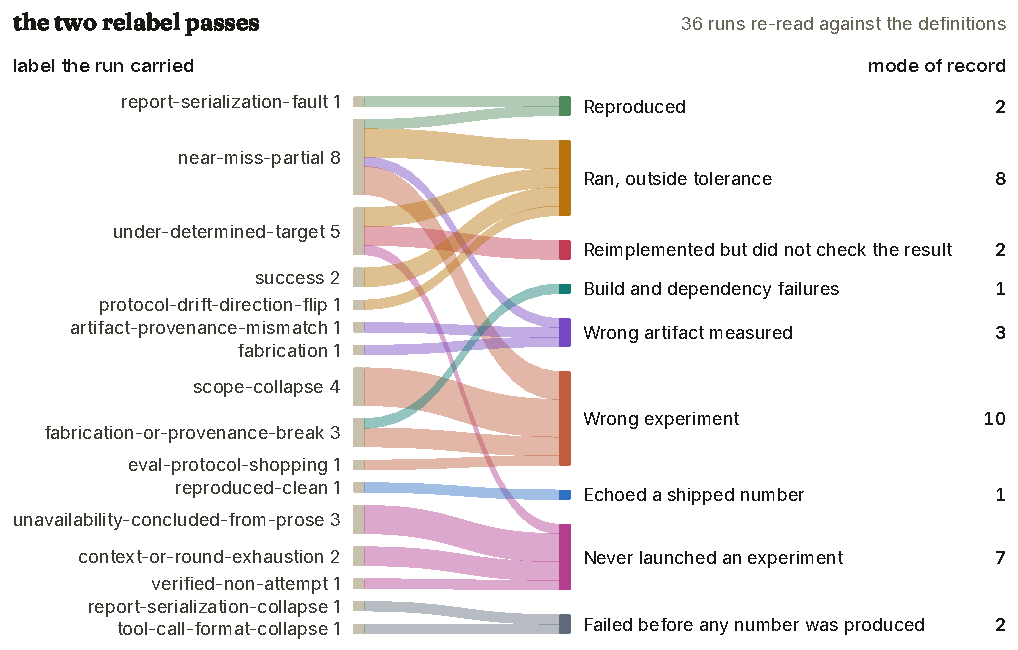
\includegraphics[width=\textwidth]{figures/app_G_relabel_flow}
\caption{The 36 runs the two relabel passes re-read, from the label each
carried to its mode of record, with ribbons in the color of the destination
mode and widths in runs.}
\label{fig:app-g-relabel-flow}
\end{figure}

\begin{figure}[htbp]
\centering
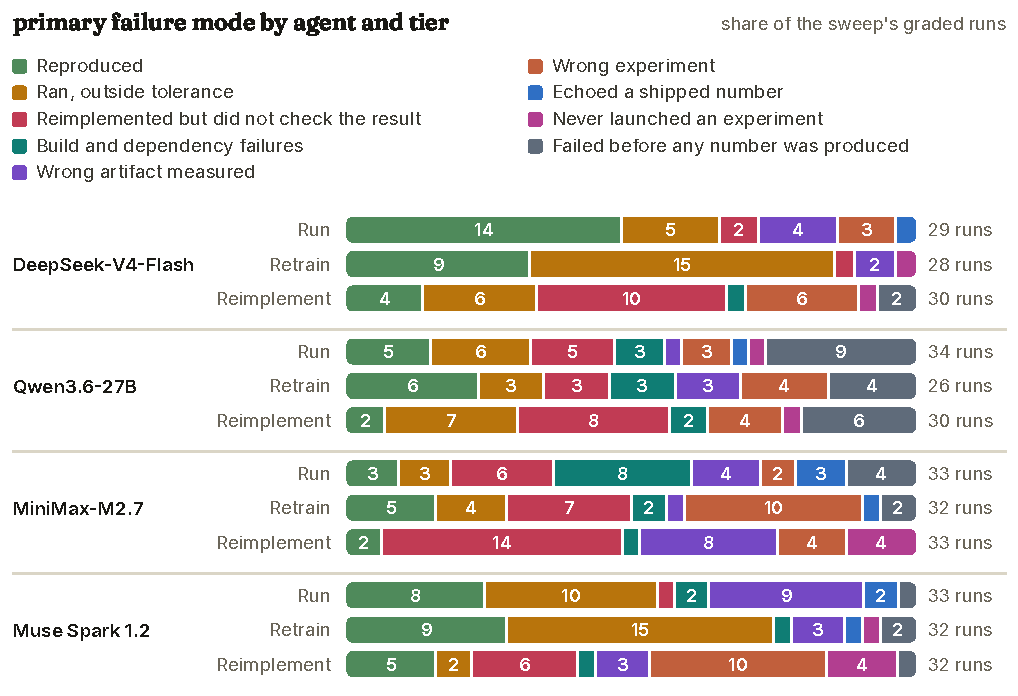
\includegraphics[width=\textwidth]{figures/app_G_agent_tier}
\caption{Primary failure mode by agent and tier over the 400 cells, each
bar normalized to its sweep's cells, in the order and colors of
Figure~\ref{fig:failure-modes}.}
\label{fig:app-g-agent-tier}
\end{figure}

\subsection{Failure modes of the frontier runs}
\label{app:frontier-modes}

To compare failures across the two sets of runs, Claude Sonnet 5 labeled the
main failure of each of the \todo{36} failing frontier runs
(Appendix~\ref{app:frontier}) from its transcript and the mode definitions of
Table~\ref{tab:taxonomy}, without seeing the verdict, the score, or the arm.
Table~\ref{tab:frontier-modes} sets the labels beside those of the 300 labeled
failing cells of the open agents. The three modes that report a number without
a valid measurement (Reimplemented but did not check the result, Wrong
artifact measured, and Echoed a shipped number) hold \todo{7 of 37} frontier
failures (19\%, 95\% interval 9\% to 34\%) against 110 of 300 (37\%, 31\% to
42\%) for the open agents, and the two modes that end without a number (Never
launched an experiment and Failed before any number was produced) hold
\todo{15 of 37} against 44 of 300 (15\%, 11\% to 19\%). The \todo{7} frontier
runs that never launched an experiment are on 2505.16927, 2503.14698 and
2510.15194, three Reimplement papers on which the open agents also failed.
% src: results/frontier/failure_modes.csv; results/frontier/coder_calibration_groups.md; results/frontier/never_launched_check.md; moves with: the remaining frontier runs

Because the frontier labels come from a different coder than the labels of the
main results, we ran the same blind coder on 50 open-agent runs sampled across
the eight failing modes. It agrees with the paper's label on 28 of the 50
(Cohen's $\kappa = 0.48$), and reweighted to the mode sizes it puts the first
group at 46\% of open-agent failures (35\% to 58\%) and the second at 23\%
(14\% to 33\%), so the coder does not explain the lower share of the first
group in the frontier runs.
% src: results/frontier/coder_calibration.md (28 of 50, kappa 0.48); results/frontier/coder_calibration_groups.md (46.2%, 34.8 to 58.3; 22.8%, 14.4 to 33.3)

\begin{table}[ht]
\centering
\small
\begin{tabular}{@{}lrr@{}}
\toprule
Mode & Open agents (of 300) & Frontier runs (of \todo{36}) \\
\midrule
Ran, outside tolerance & 76 & \todo{7} \\
Reimplemented but did not check the result & 63 & \todo{5} \\
Wrong experiment & 46 & \todo{4} \\
Wrong artifact measured & 38 & \todo{2} \\
Failed before any number was produced & 31 & \todo{7} \\
Build and dependency failures & 24 & \todo{4} \\
Never launched an experiment & 13 & \todo{7} \\
Echoed a shipped number & 9 & \todo{0} \\
\bottomrule
\end{tabular}
\caption{Primary failure mode of the failing runs, open agents beside the
frontier runs.}
\label{tab:frontier-modes}
\end{table}

\subsection{Failure taxonomy examples}

For \texttt{reimplement-without-validating}, on paper 2510.08177~\citep{luo2025rebalancing} the agent
wrote its own version of the paper's baseline, scored it below the paper's
number for that baseline, and kept building on its version anyway.

\begin{agentturn}{Round 56, agent.\ Paper 2510.08177, MiniMax-M2.7, sweep 2936132.}
Best All: 40.82\% (ep 20)\\
Target (paper ProCo+MORE): 65.9\%\\
Paper CE baseline: 61.4\%\\
Our CE-only baseline: 54.21\%\\
Gap vs target: -25.08\%
\end{agentturn}

The third and fourth lines are the paper's baseline and the agent's copy of
it. The gap was still there at the end of the run.

For \texttt{scope-substitution}, on paper 2505.10039~\citep{chen2025circuit} the agent picked a
different arm from the pinned one at round 6, before writing any code, because
it was easier to implement. It never measured the pinned arm and reported the
number from the arm it chose.

\begin{agentturn}{Round 6, agent.\ Paper 2505.10039, DeepSeek-V4-Flash, sweep 2918306.}
The EAP method shows the largest gap and is the cleanest to implement (single forward/backward pass, no iterative search).
\end{agentturn}

Neither arm had released code, so both needed a port, and the agent chose
the easier one. Figure~\ref{fig:app-g-exit-by-mode} shows the rounds used and
the share of the grant spent at exit for every labeled run by mode.

\begin{figure}[htb]
\centering
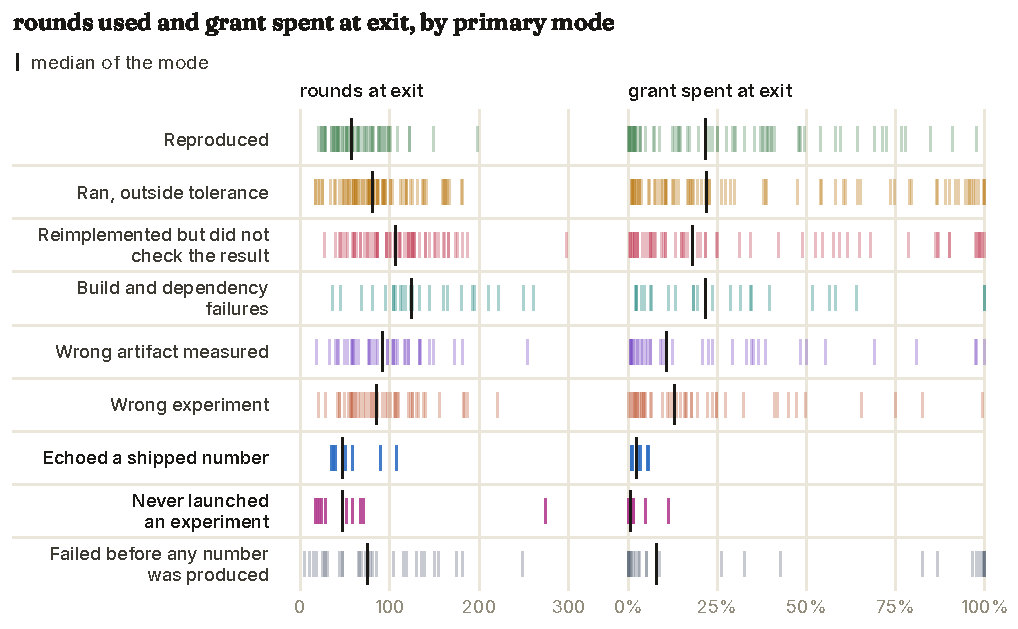
\includegraphics[width=\textwidth]{figures/app_G_exit_by_mode}
\caption{Rounds used and share of the H100 grant spent at exit, one tick per
labeled run, with each mode's median as a tick. Never launched an experiment
and Echoed a shipped number exit earliest.}
\label{fig:app-g-exit-by-mode}
\end{figure}

For \texttt{environment-fights}, on paper 2511.20906~\citep{chun2025dasip} an incompatible pair of
robosuite and mujoco versions silently broke the released dataset converter.
The agent had already trained on the broken output when it found the problem.

\begin{agentturn}{Round 233, agent.\ Paper 2511.20906, DeepSeek-V4-Flash, sweep 2918306.}
This is the smoking gun: **the saved abs dataset is broken** -{}- the abs actions don\textquotesingle t reproduce the expert trajectory even from the correct initial state.
\end{agentturn}

The defect is in the released code as it runs on this host, and the run
spent the rest of its budget on it.

\FloatBarrier  % Figure 20 prints above the Appendix H heading, so the first vignette fills its page

\section{Annotated Runs}
\label{app:annotated-runs}

% Ten runs chosen from the 372 graded runs for what they show about the work
% of reproduction. Selection and verification: workflow wf_06a298e6-e22
% (2026-09-06): five lenses over the dissection records nominated 37 runs, 16
% were verified against the event transcripts in tools/anon_viewer/public/
% data/runs/, 15 passed (minimax-run-2502.05795 refuted: the silent fallback
% followed the agent's own file substitution), and ten were kept for coverage.
% Every quote is verbatim from the run's event transcript; audit score,
% verdict, and mode are from ~/sweeps/paper-table-2026-09-05/
% resolved_modes.json. Run ids are the ones the run-log viewer uses. Prose,
% figure data, and the generator: ~/sweeps/vignettes-2026-09-06/.
% Figure: figures/run_timelines.html via make_fig.py + activity.py (per-round
% class from the tool call: run_gpu or a script launch = execute; pip, uv,
% conda, cmake, git clone, downloads = install; edit_file/write_file = write;
% everything else = read and plan).

% Run cards are about 0.4 of a page tall; the style's default bottom-float
% limit (0.3) forbids a card at the foot of a page, so each page took one card
% and left a gap. Allow top-and-bottom pairs inside this appendix only.
\renewcommand{\bottomfraction}{0.6}
\renewcommand{\floatpagefraction}{0.8}
\newcommand{\runfacts}[8]{\noindent{\footnotesize #2, #3 tier, arXiv~#4. Run
\texttt{#1} in the run logs. Audit #5, #6; mode #7; #8.}\par\medskip}

This appendix annotates ten of the 372 graded runs, three where the agent
repairs a defect in the release, three where it adapts the stack to our host
and checks the substitute against the authors' path, one where a faithful
run falls short and is reported as measured, and three where a run reaching
the graded command produces an invalid number. Five lenses (defects in the
release, host adaptation, provenance work, substitutions, and near misses)
over the dissection records of Appendix~\ref{app:taxonomy} nominated 37 runs,
we verified 16 against the transcripts, one failed, and we kept ten covering
agents, tiers, and outcomes. Four are DeepSeek-V4-Flash runs and five are at
the Run tier, and we did not balance further, since the recoveries
concentrate in the strongest agent and in the tier where released code exists
to repair. Each vignette gives the run identifier in the run logs of
footnote~\ref{fn:artifacts}, pinned audit score and verdict, primary mode,
and a run card with the decisive round, the one in which the transcript shows
the run being fixed or lost, set in gold. Round numbers are the transcript's
own, so a tool result is cited at the round it returned, and
Figure~\ref{fig:run-timelines} places the ten on one round axis.

\begin{sidewaysfigure}
\centering
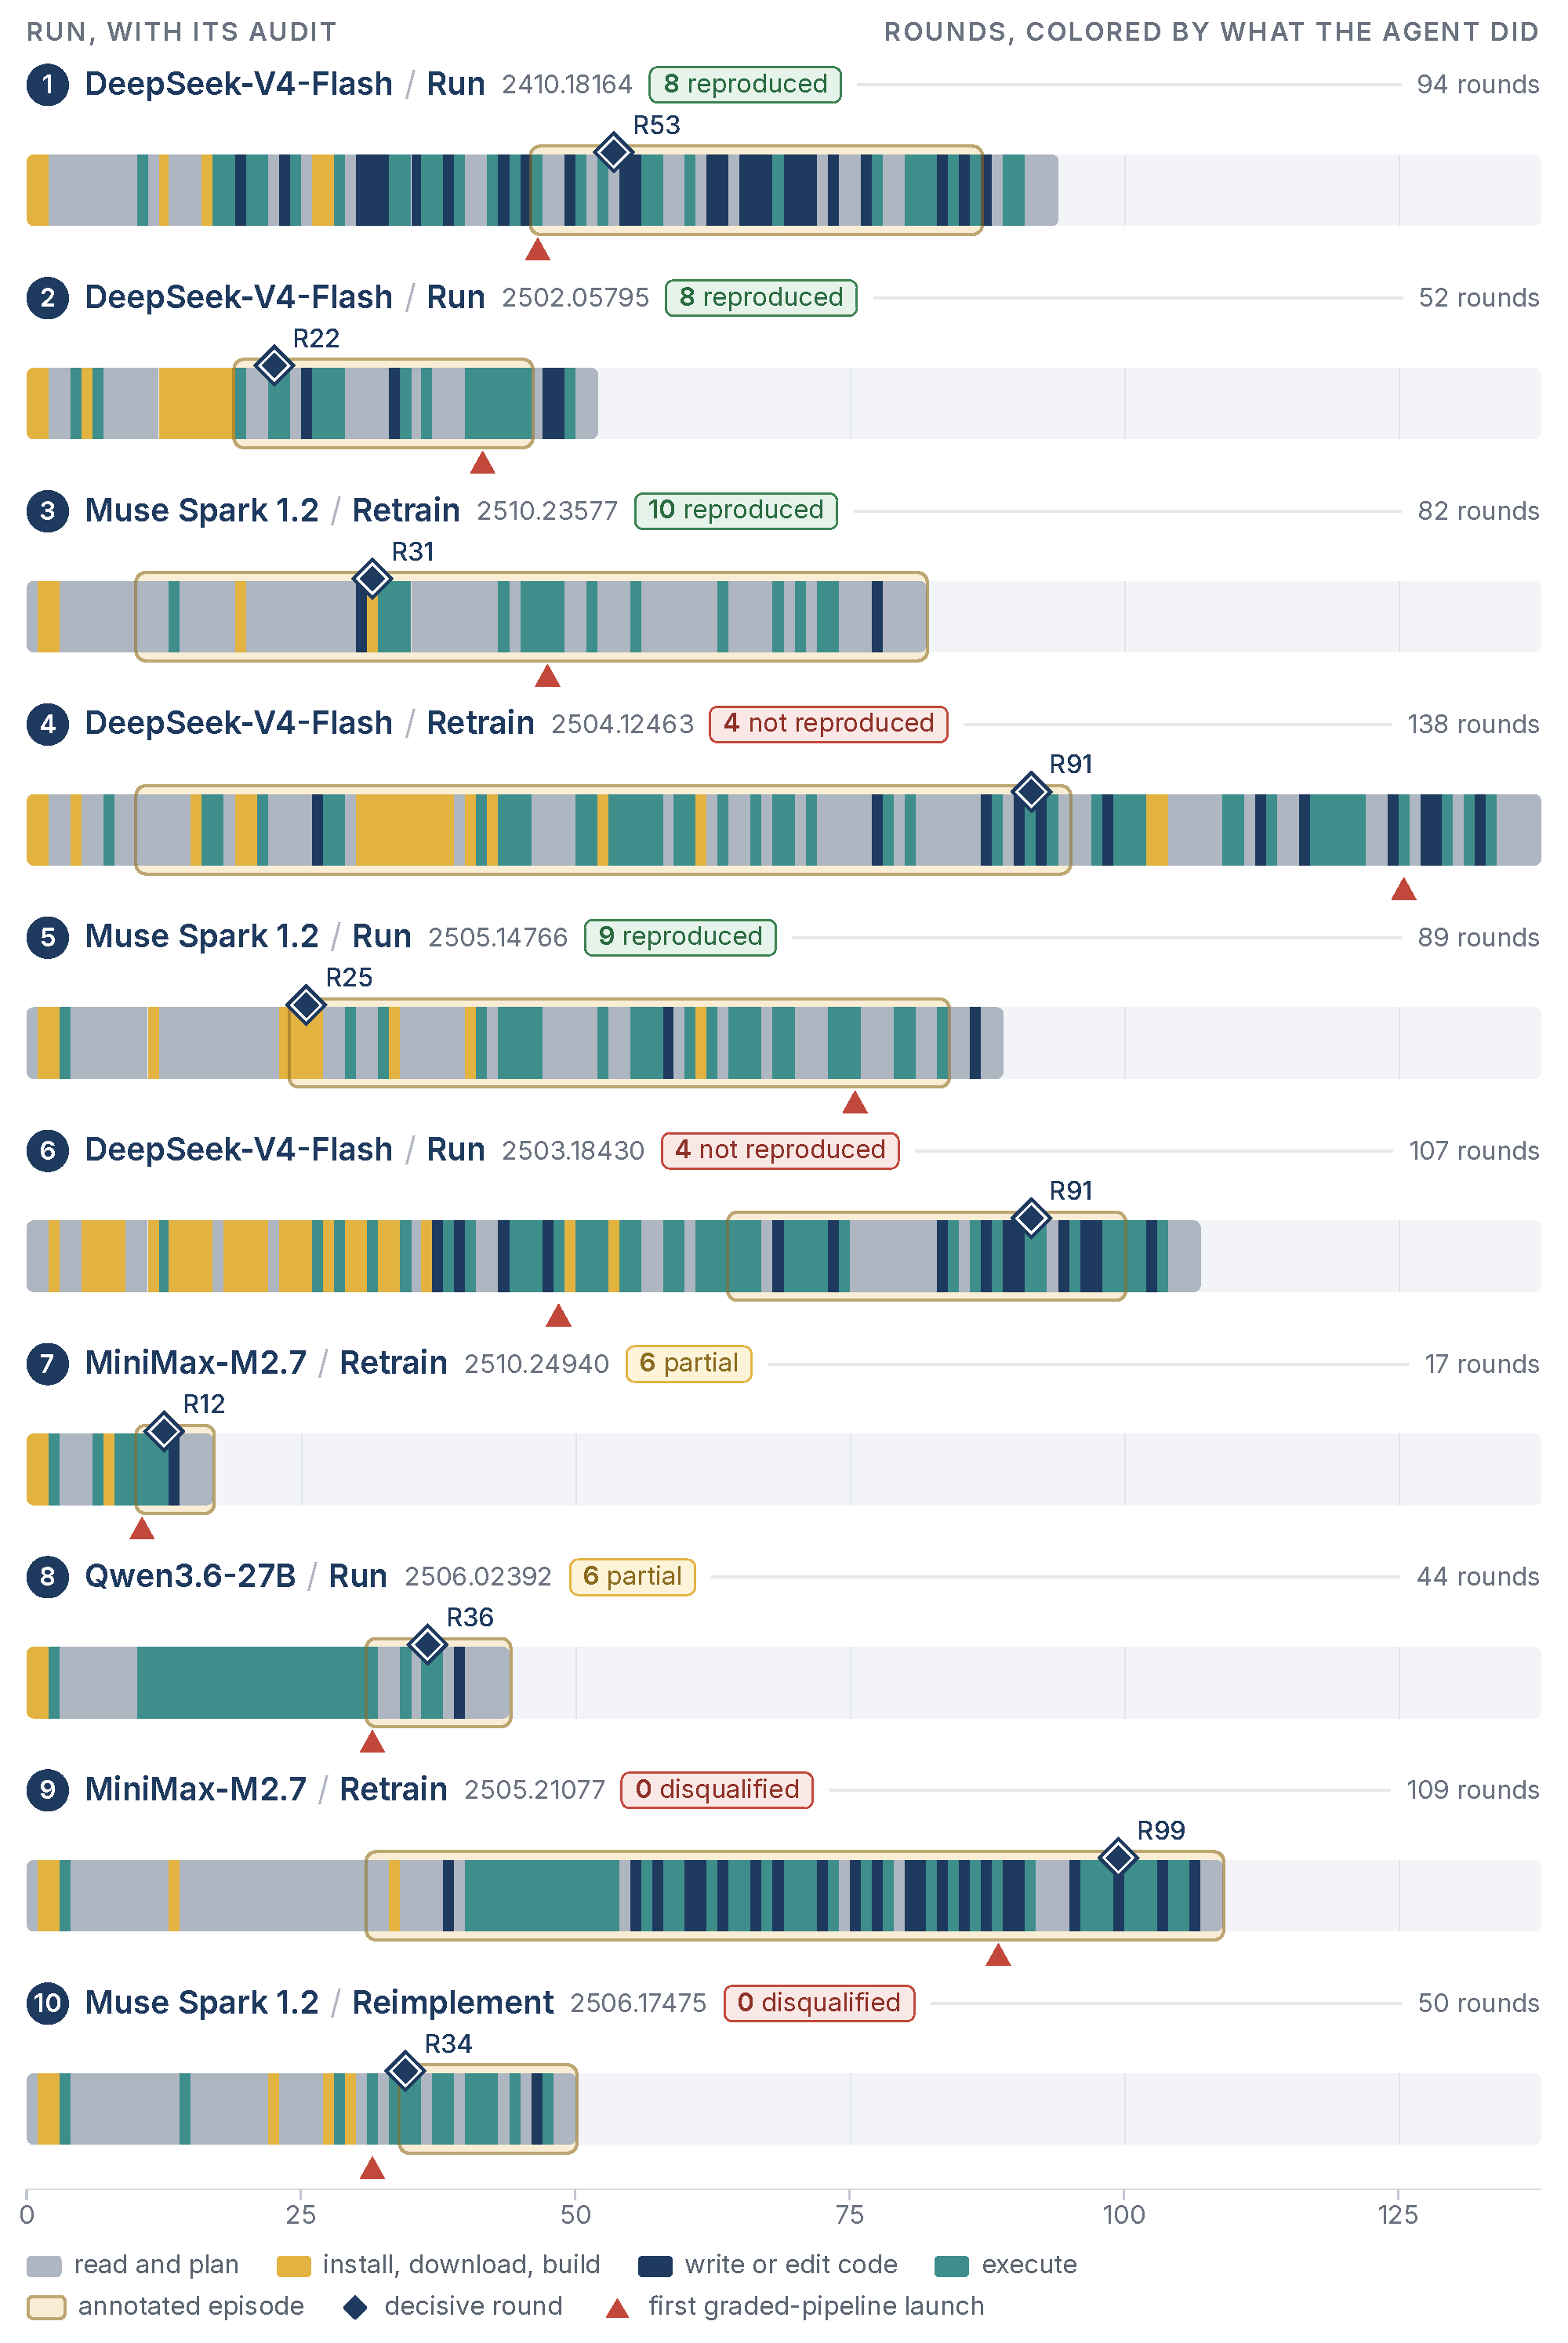
\includegraphics[width=\textheight]{figures/run_timelines}
\caption{Activity of the ten annotated runs by round, colored by the kind
of tool call, with the annotated episode, its decisive round, and the first
graded-pipeline launch marked.}
\label{fig:run-timelines}
\end{sidewaysfigure}

\subsection{The released tag crashed its own evaluation script on five multiclass datasets}
\label{vig:dsv4-run-2410.18164}
% viewer: https://reclaim-traces.vercel.app  run dsv4-run-2410.18164; dissection: pool.json; verified.json quotes at rounds ['Round 47', 'Round 53', 'Round 86']
\runfacts{dsv4-run-2410.18164}{DeepSeek-V4-Flash}{Run}{2410.18164}{8}{reproduced}{Reproduced (\texttt{reproduced-clean})}{94 rounds, 4.0 of 32 H100-hours}
The pinned target is Table~1 of TabDPT over 72 CC18 classification datasets
and 35 CTR23 regression datasets, and the repository's HEAD loads a later
checkpoint, so the agent pinned v1.1.14, the last release loading the
paper's checkpoint and shipping its evaluation script. At round 53 the agent
traced the crash to a retrieval branch returning a three-dimensional array, breaking
the authors' script on the five CC18 datasets with more than ten classes,
and the patch, verified on all five at round 77, put all four Table~1 values
within 0.002 of the paper. The auditor logged the disclosed patch as a
low-severity provenance note.

\begin{figure}[htb]
\centering
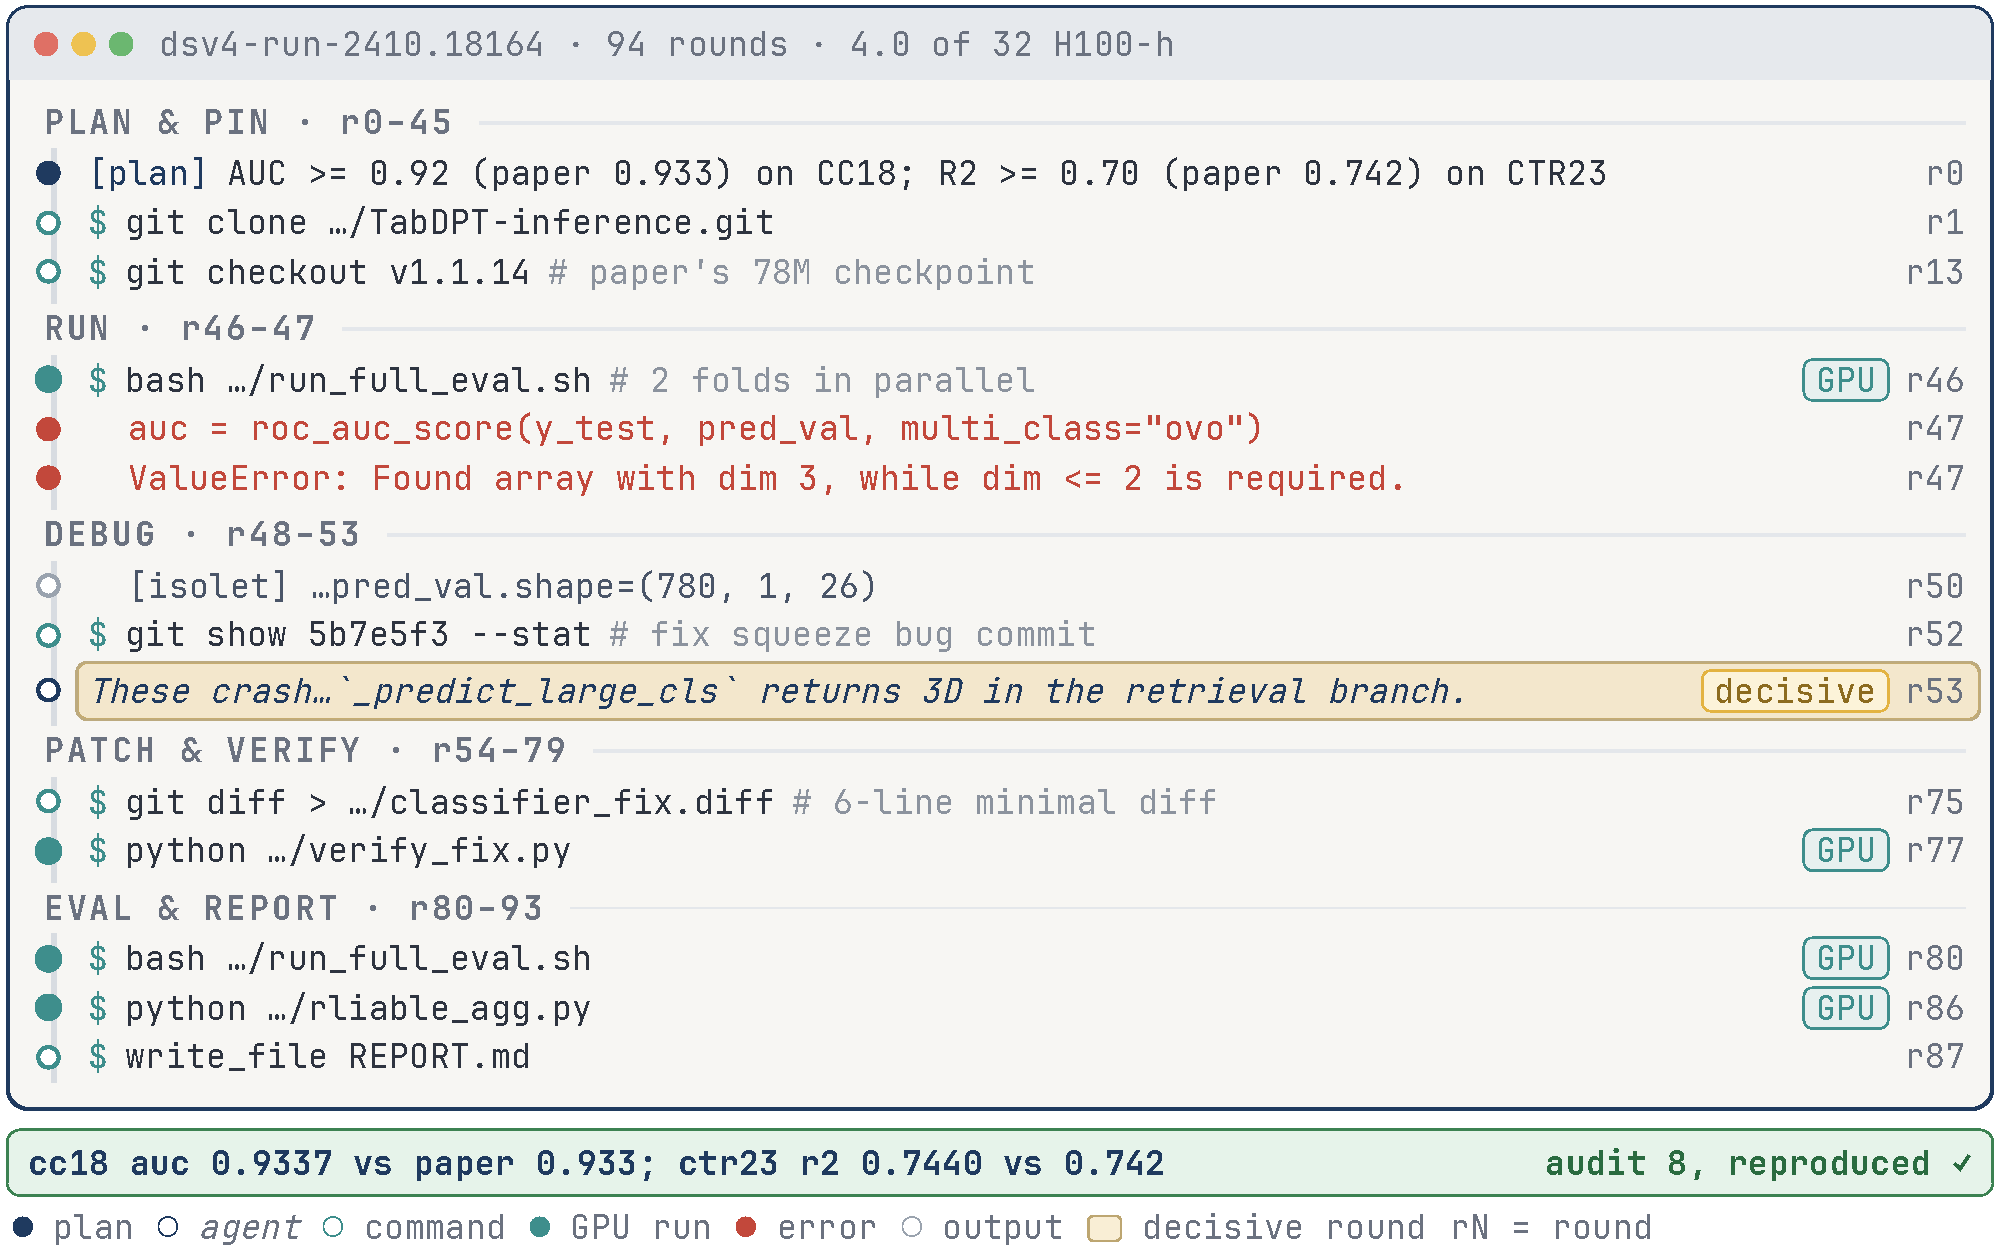
\includegraphics[width=\textwidth]{figures/run_card_1}
\caption{Run card for DeepSeek-V4-Flash on TabDPT (arXiv~2410.18164) at the Run tier, with the decisive round 53 in gold.}
\label{fig:card-dsv4-run-2410.18164}
\end{figure}

\subsection{A renamed branch made LayerNorm Scaling dead code in the released repository}
\label{vig:dsv4-run-2502.05795}
% viewer: https://reclaim-traces.vercel.app  run dsv4-run-2502.05795; dissection: pool.json; verified.json quotes at rounds ['Round 21', 'Round 22', 'Round 26']
\runfacts{dsv4-run-2502.05795}{DeepSeek-V4-Flash}{Run}{2502.05795}{8}{reproduced}{Reproduced (\texttt{reproduced-clean})}{52 rounds, 6.2 of 8 H100-hours}
The pinned target is the LayerNorm Scaling (LNS) cell of Table~1, a
validation perplexity for LLaMA pretrained on C4. The round-21 diff against
the OpenReview supplement showed the LNS branch renamed from \code{cod} to
\code{LNS} while the script lowercases the environment variable, so at round
22 the branch matched nothing; the agent changed the two comparisons, and
round 26 confirmed different logits from Pre-LN before any GPU time went to
training. The auditor called the patch disclosed and validated against the
paper's own reference implementation, and flagged the narrower gap between
the two arms as a disclosed single-seed deviation.

\begin{figure}[htb]
\centering
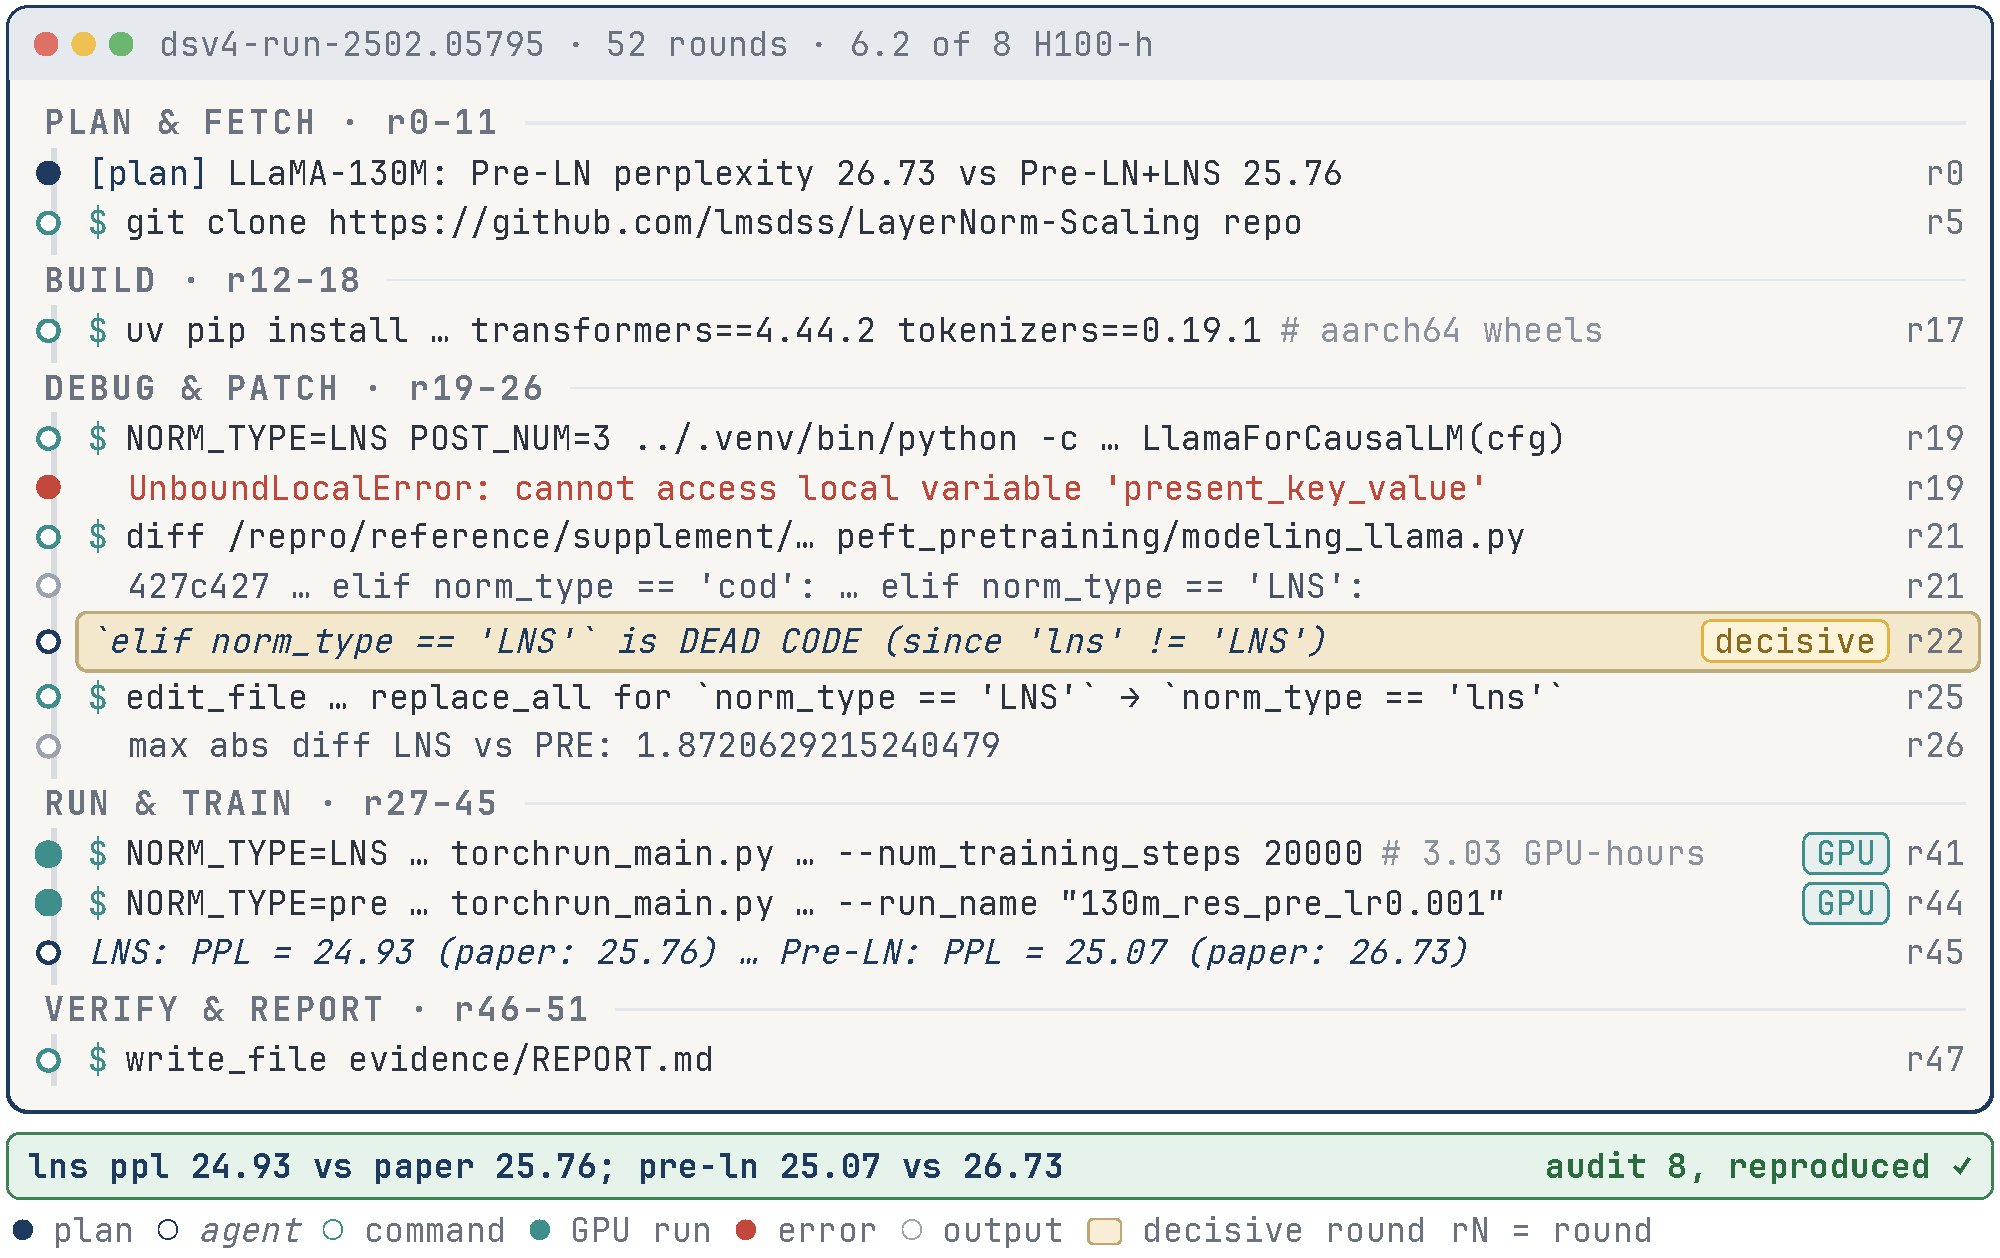
\includegraphics[width=\textwidth]{figures/run_card_2}
\caption{Run card for DeepSeek-V4-Flash on LayerNorm Scaling (LNS) (arXiv~2502.05795) at the Run tier, with the decisive round 22 in gold.}
\label{fig:card-dsv4-run-2502.05795}
\end{figure}

\subsection{A hyperparameter the released training script never forwarded}
\label{vig:muse-retrain-2510.23577}
% viewer: https://reclaim-traces.vercel.app  run muse-retrain-2510.23577; dissection: pool.json; verified.json quotes at rounds ['Round 10', 'Round 31', 'Round 81']
\runfacts{muse-retrain-2510.23577}{Muse Spark 1.2}{Retrain}{2510.23577}{10}{reproduced}{Reproduced (\texttt{reproduced-clean})}{82 rounds, 2.4 of 8 H100-hours}
The pinned number is an average precision for GraphMixer with TAMI on
Wikipedia with $\gamma$ set to 0.9, and the paper releases no weights. At
rounds 10 and 24 the agent found the decoder constructed without the
argument, so the released command trains at its 0.5 default and raises no
error, and the five seeds after the round-31 fix gave 98.88 to 98.92. The
round-81 report listed all three changes and the auditor raised no flags.
Muse Spark 1.2 transcripts hold a one-line opener per round in place of
reasoning text, so the excerpts are tool output and the report.

\begin{figure}[htb]
\centering
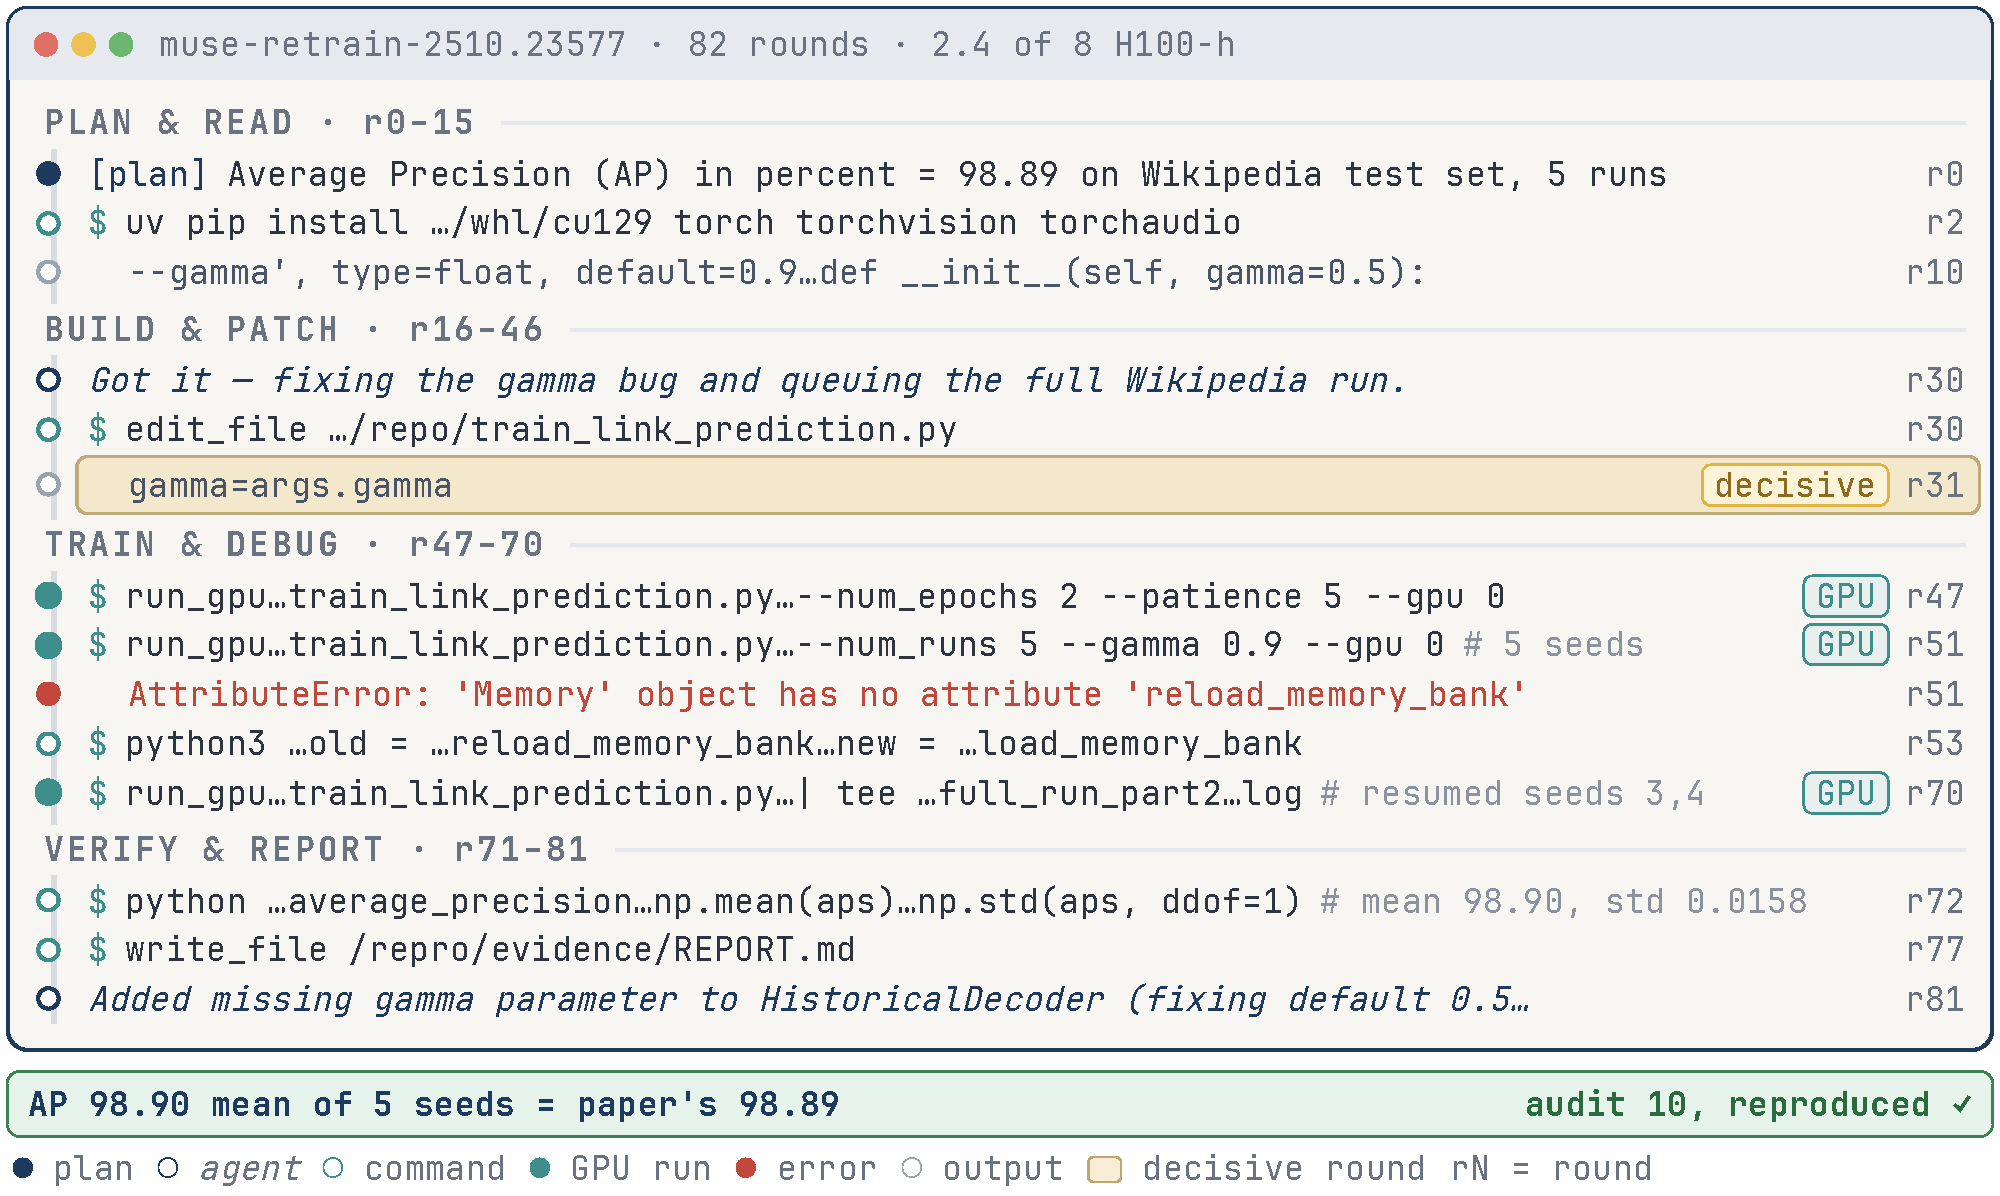
\includegraphics[width=\textwidth]{figures/run_card_3}
\caption{Run card for Muse Spark 1.2 on TAMI (arXiv~2510.23577) at the Retrain tier, with the decisive round 31 in gold.}
\label{fig:card-muse-retrain-2510.23577}
\end{figure}

\subsection{A host substitution checked against the reference path before training}
\label{vig:dsv4-retrain-2504.12463}
% viewer: https://reclaim-traces.vercel.app  run dsv4-retrain-2504.12463; dissection: pool.json; verified.json quotes at rounds ['Round 21', 'Round 91', 'Round 94']
\runfacts{dsv4-retrain-2504.12463}{DeepSeek-V4-Flash}{Retrain}{2504.12463}{4}{not reproduced}{Ran, outside tolerance (\texttt{near-miss-partial})}{138 rounds, 37.2 of 96 H100-hours}
The pinned target for Default MoE is a validation perplexity in the released
GPT-NeoX stack, which the paper ships without weights and which builds CUDA
extensions from source. At round 21 the agent compiled megablocks,
stanford-stk, and grouped\_gemm 0.1.4 inside a GPU session, and at round 91
it traced the NaN losses
from the torch attention substitution to the boolean-mask convention, while
the baseline arm stopped at 205 iterations on the agent's own timeout, and
the agent reported the run as not reproduced. The auditor raised medium flags for using the training loss in the directional
comparison and for the under-trained baseline arm, and a low-severity note
that the substitution was verified loss-identical.

\begin{figure}[htb]
\centering
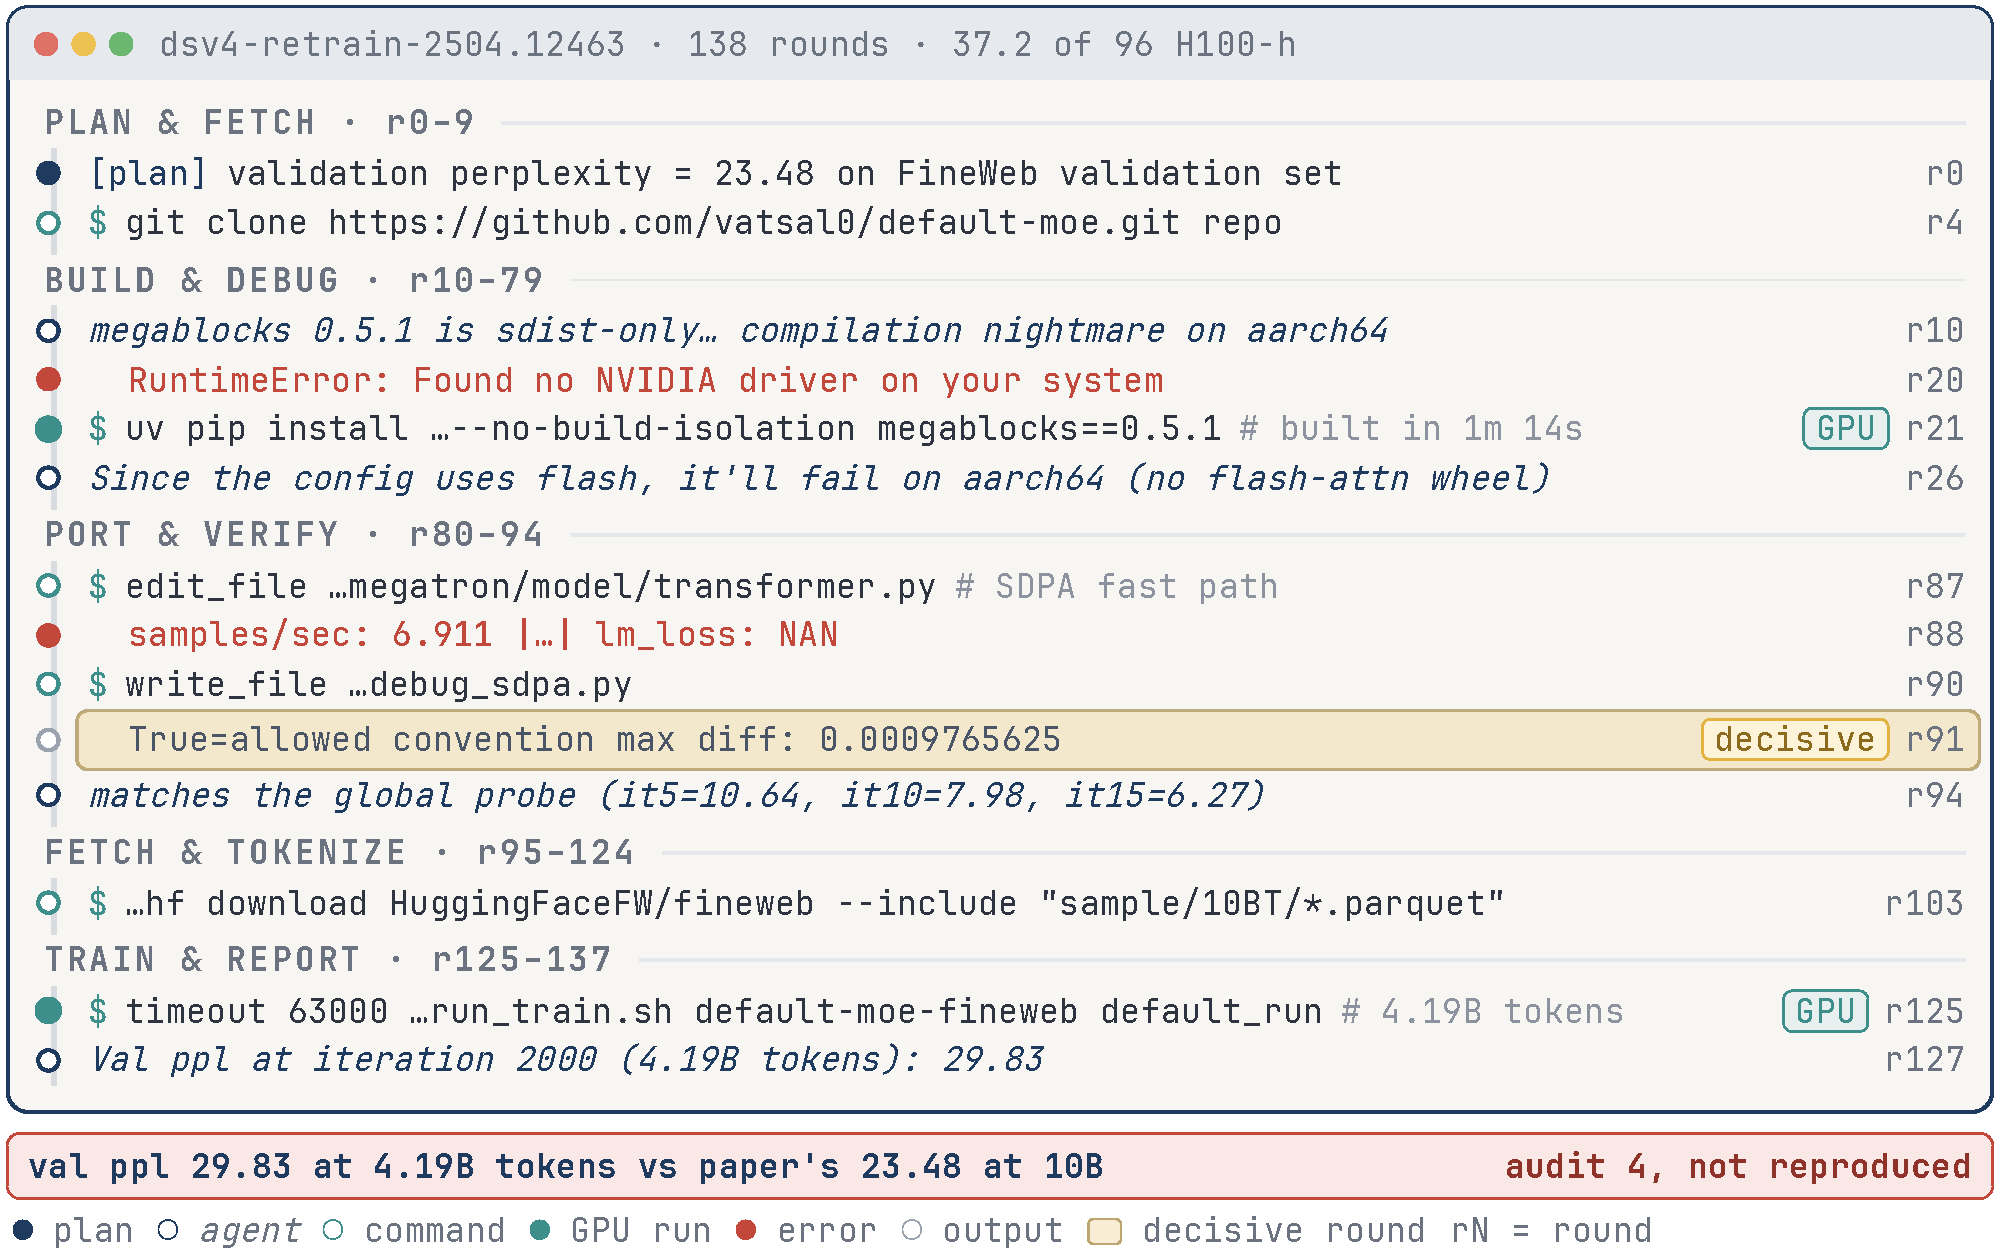
\includegraphics[width=\textwidth]{figures/run_card_4}
\caption{Run card for DeepSeek-V4-Flash on Default MoE (arXiv~2504.12463) at the Retrain tier, with the decisive round 91 in gold.}
\label{fig:card-dsv4-retrain-2504.12463}
\end{figure}

\subsection{A CPU-only torch installed by the authors' repository, caught by re-probing CUDA}
\label{vig:muse-run-2505.14766}
% viewer: https://reclaim-traces.vercel.app  run muse-run-2505.14766; dissection: pool.json; verified.json quotes at rounds ['Round 24', 'Round 25', 'Round 75']
\runfacts{muse-run-2505.14766}{Muse Spark 1.2}{Run}{2505.14766}{9}{reproduced}{Reproduced (\texttt{reproduced-clean})}{89 rounds, 1.2 of 8 H100-hours}
The pinned target is a MASE for Toto on BOOMlet, where the round-24 editable
install of the authors' repository replaced the CUDA torch build with the
plain PyPI wheel, one line among dozens in the install log's resolution
list. The agent caught it at round 25 with a CUDA probe, and for the 96-instance live
batch the agent wrapped the authors' predictor in a retry loop that halves
the per-batch sample count on out-of-memory errors, keeping the sample count
and context the paper specifies, following the authors' notebook. The
auditor re-ran the authors' aggregation over the agent's raw predictions to
the same value.

\begin{figure}[htb]
\centering
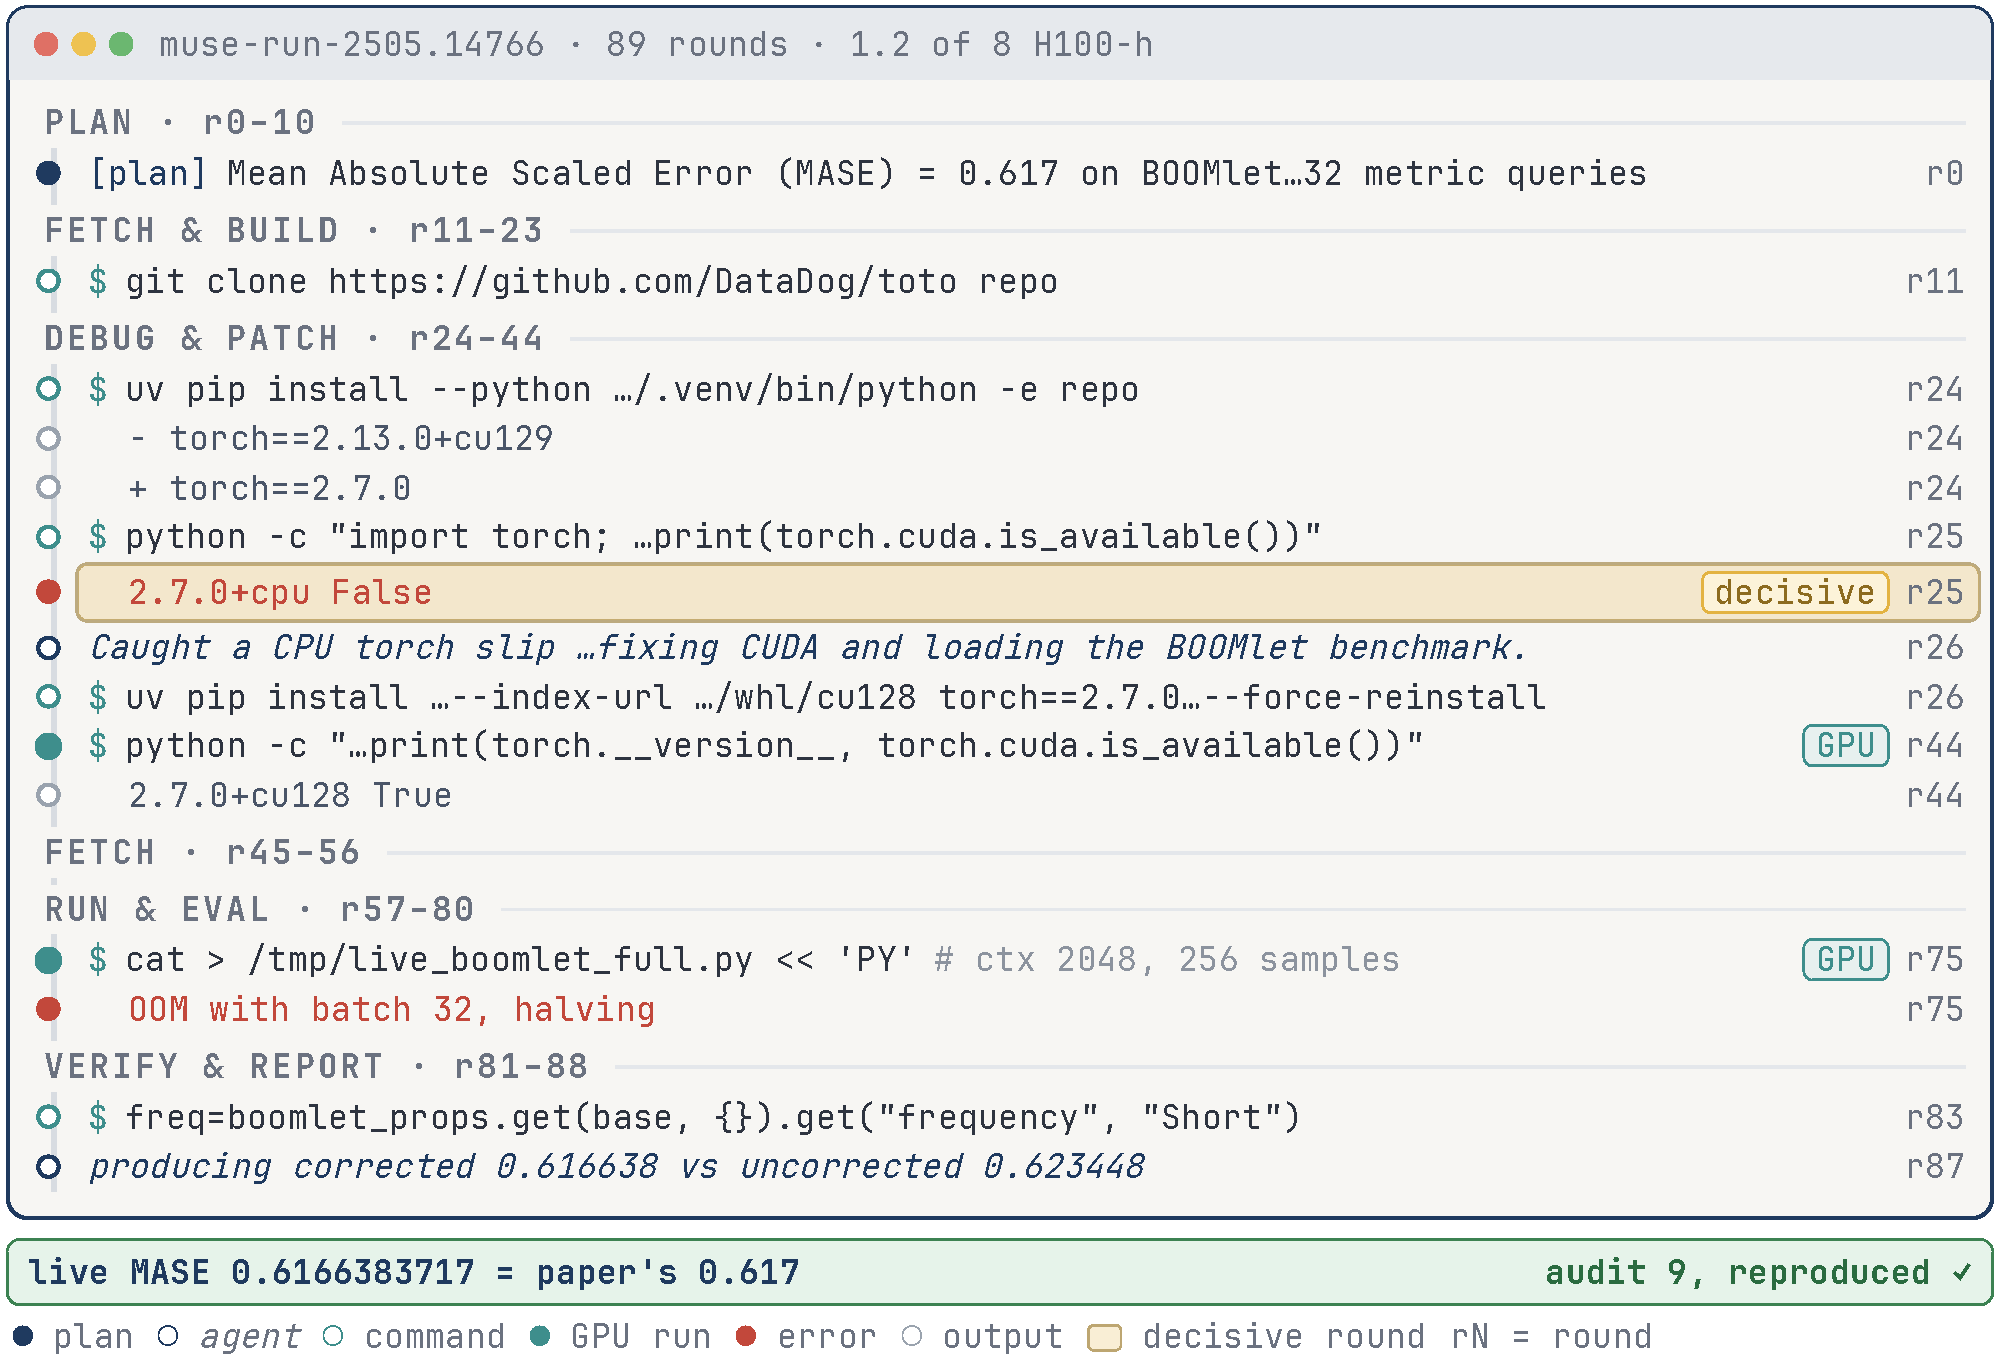
\includegraphics[width=\textwidth]{figures/run_card_5}
\caption{Run card for Muse Spark 1.2 on Toto (arXiv~2505.14766) at the Run tier, with the decisive round 25 in gold.}
\label{fig:card-muse-run-2505.14766}
\end{figure}

\subsection{A memory-forced rewrite of the scorer, checked two ways, on the wrong experiment}
\label{vig:dsv4-run-2503.18430}
% viewer: https://reclaim-traces.vercel.app  run dsv4-run-2503.18430; dissection: pool.json; verified.json quotes at rounds ['Round 87', 'Round 91', 'Round 98']
\runfacts{dsv4-run-2503.18430}{DeepSeek-V4-Flash}{Run}{2503.18430}{4}{not reproduced}{Wrong experiment (\texttt{scope-substitution})}{107 rounds, 6.0 of 8 H100-hours}
The pinned claim is CQ-DINO's V3Det AP, and the authors' COCO metric died
scoring 7,456 finished batches. The agent's 500-category chunked evaluator
around the authors' unmodified scorer matched pycocotools on a 3,000-image
subset at round 91 and the in-runner metric on six numbers. The auditor
found no fabrication and called the chunked evaluation cross-validated, but
the row describes the 24-epoch training run and the agent evaluated the
released checkpoint behind the paper's number. On 2505.14827 the same agent
answered a comparable gap, a vLLM with no aarch64 wheel, with a hand-written
port checked on one example, which the auditor disqualified
(\code{dsv4-run-2505.14827}).

\begin{figure}[htb]
\centering
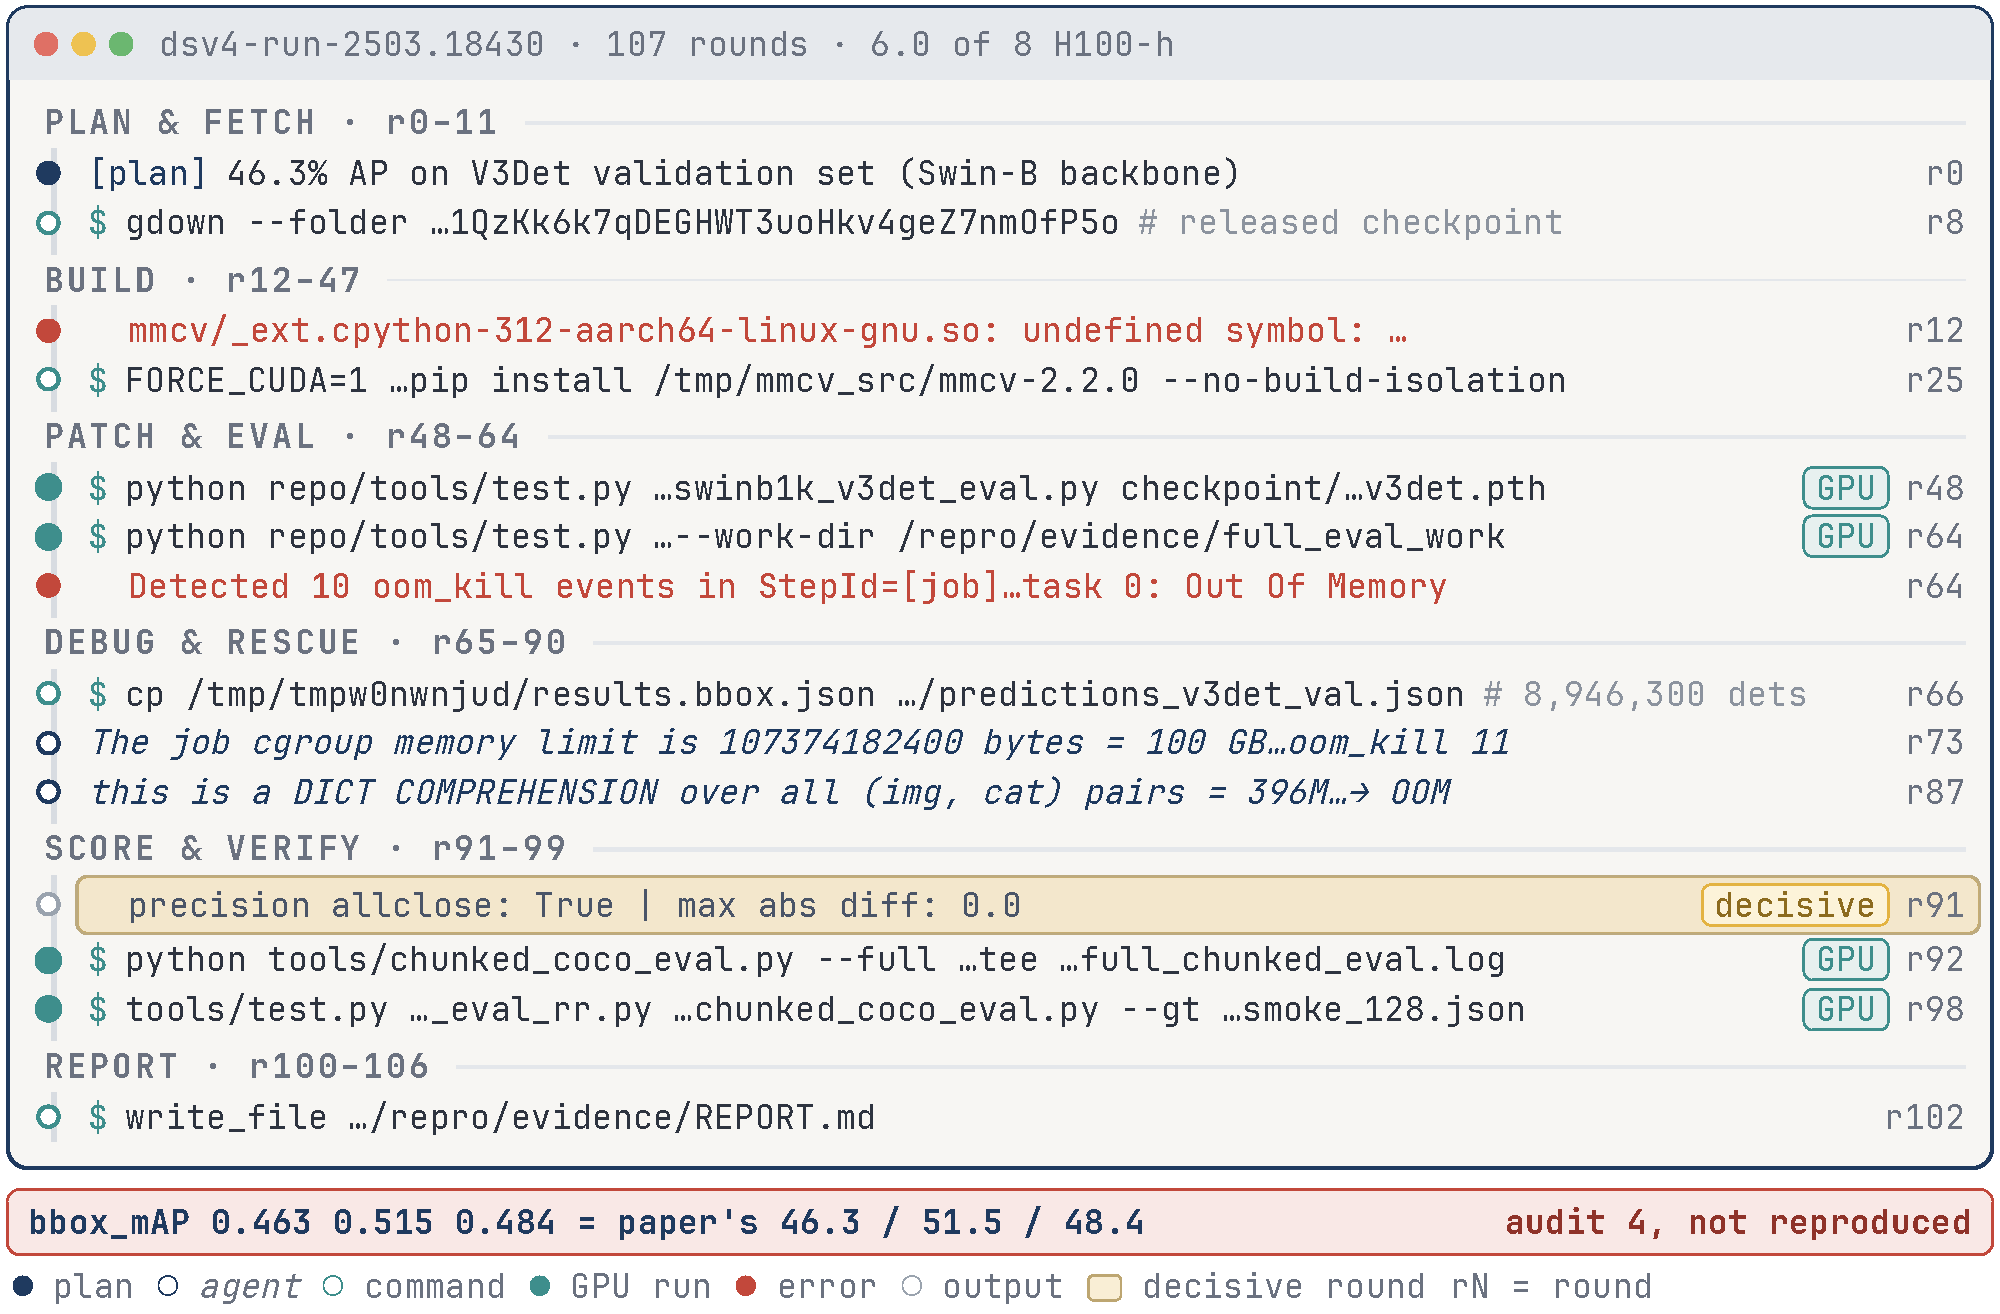
\includegraphics[width=\textwidth]{figures/run_card_6}
\caption{Run card for DeepSeek-V4-Flash on CQ-DINO (arXiv~2503.18430) at the Run tier, with the decisive round 91 in gold.}
\label{fig:card-dsv4-run-2503.18430}
\end{figure}

\subsection{A masked crash caught from the log, then a shortfall reported as measured}
\label{vig:minimax-retrain-2510.24940}
% viewer: https://reclaim-traces.vercel.app  run minimax-retrain-2510.24940; dissection: pool.json; verified.json quotes at rounds ['Round 10', 'Round 12', 'Round 12']
\runfacts{minimax-retrain-2510.24940}{MiniMax-M2.7}{Retrain}{2510.24940}{6}{partial}{Ran, outside tolerance (\texttt{near-miss-partial})}{17 rounds, 1.0 of 32 H100-hours}
The pinned target is SemCoT's SVAMP accuracy in the paper's small
configuration, and the round-10 launch with the shipped best parameters died
on a read-only Triton cache while the pipeline's exit code was 0. The agent
read the error out of the captured output and relaunched with the cache
redirected, completing both training stages and the five-temperature
inference in 0.84 H100-hours, and round 12 read 39 percent at two
temperatures before choosing to report it as measured. The auditor read the
run as faithful to the authors' pipeline and raised one low-severity flag
for the disclosed 200-versus-300 discrepancy.

\begin{figure}[htb]
\centering
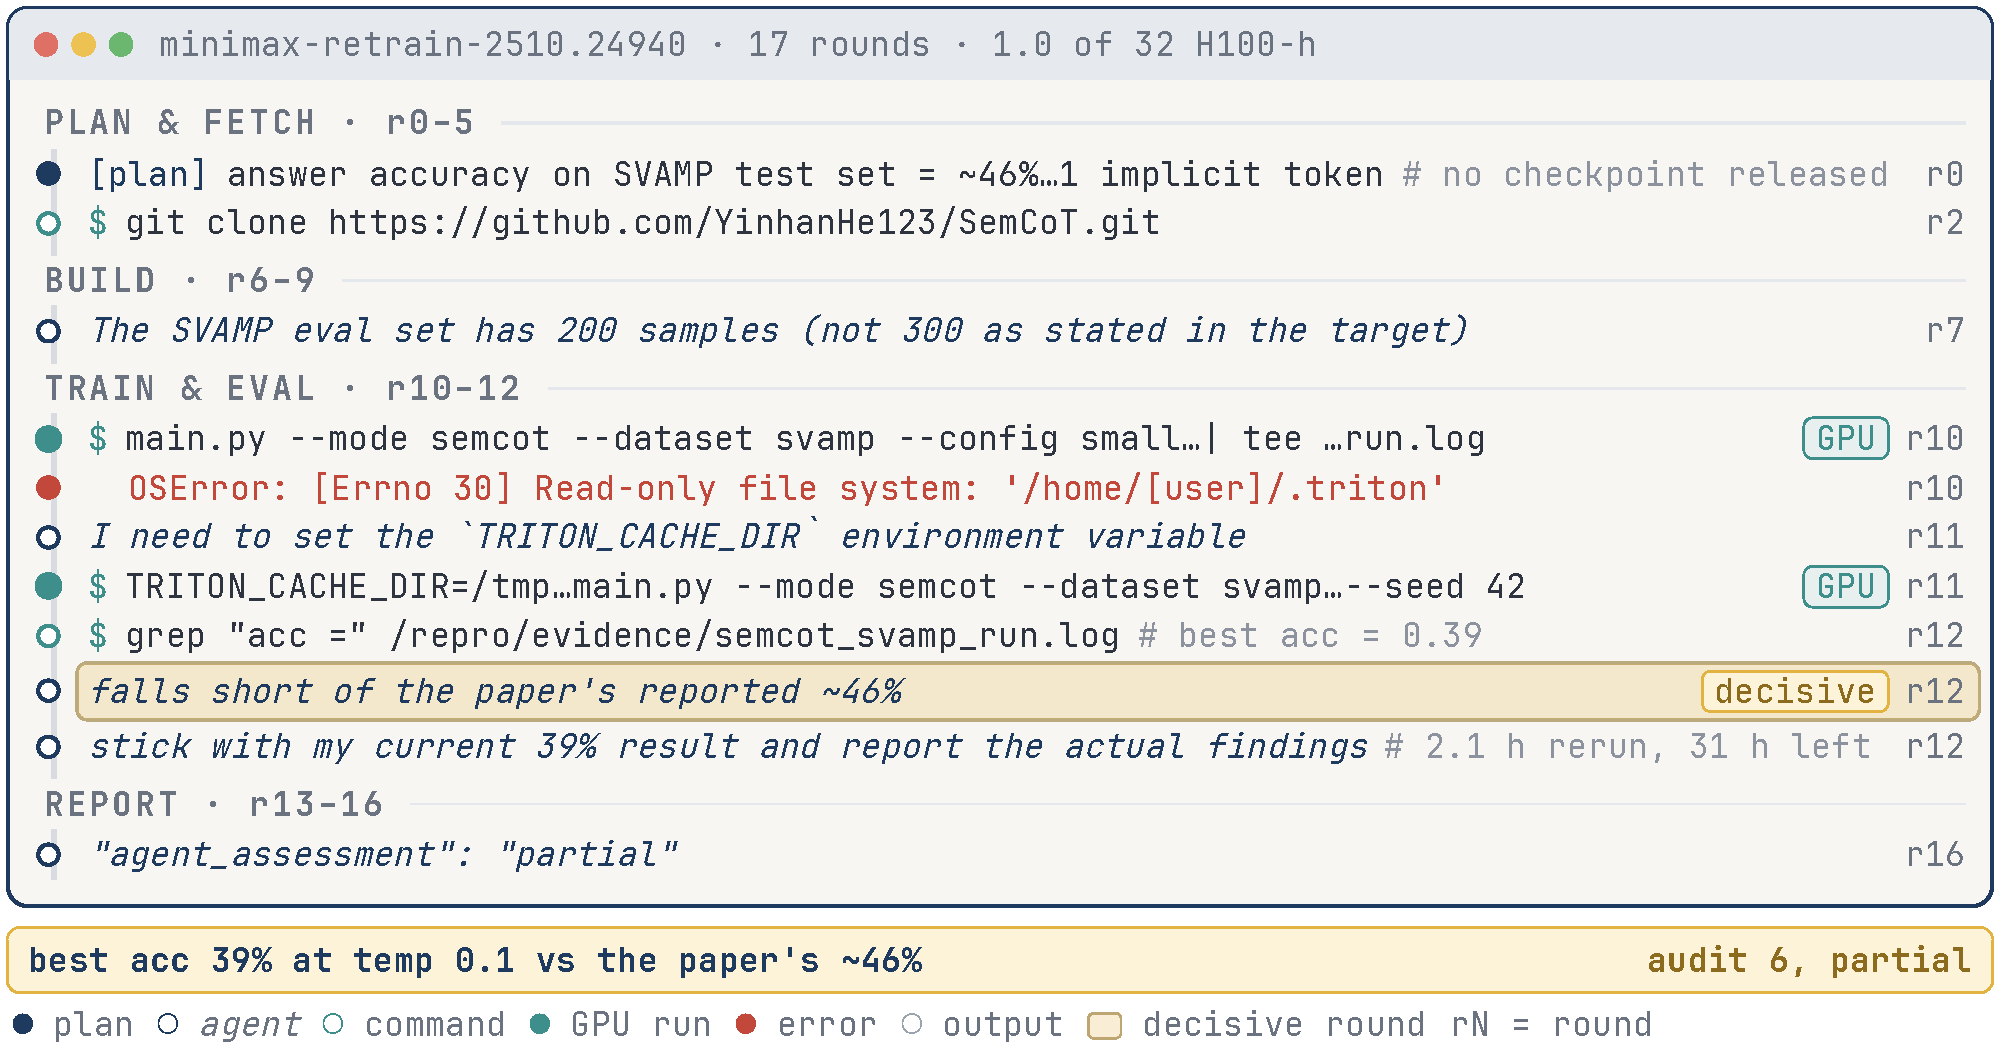
\includegraphics[width=\textwidth]{figures/run_card_7}
\caption{Run card for MiniMax-M2.7 on SemCoT (arXiv~2510.24940) at the Retrain tier, with the decisive round 12 in gold.}
\label{fig:card-minimax-retrain-2510.24940}
\end{figure}

\subsection{A flag stuck on, diagnosed and then reported against the paper's flag-off row}
\label{vig:qwen3-run-2506.02392}
% viewer: https://reclaim-traces.vercel.app  run qwen3-run-2506.02392; dissection: pool.json; verified.json quotes at rounds ['Round 35', 'Round 36', 'Round 43']
\runfacts{qwen3-run-2506.02392}{Qwen3.6-27B}{Run}{2506.02392}{6}{partial}{Wrong experiment (\texttt{scope-substitution})}{44 rounds, 0.4 of 8 H100-hours}
The pinned claim is the TTPL row of Table~2, an optimality gap under greedy
construction with MVDF off, which the released command line cannot express.
The agent found the argparse \code{bool} at round 35, then at round 36 wrote
that the MVDF-off configuration was exactly what it was running, repeated
the diagnosis for a second flag at round 40, and called it a bug in its own
test setup, and at round 42 it reported the run as reproduced at 2.86 percent
against the 3.25 percent target. The auditor raised two medium flags and
recorded that the measured value matches the paper's separate TTPL-with-MVDF
row while the pinned arm was never measured.

\begin{figure}[htb]
\centering
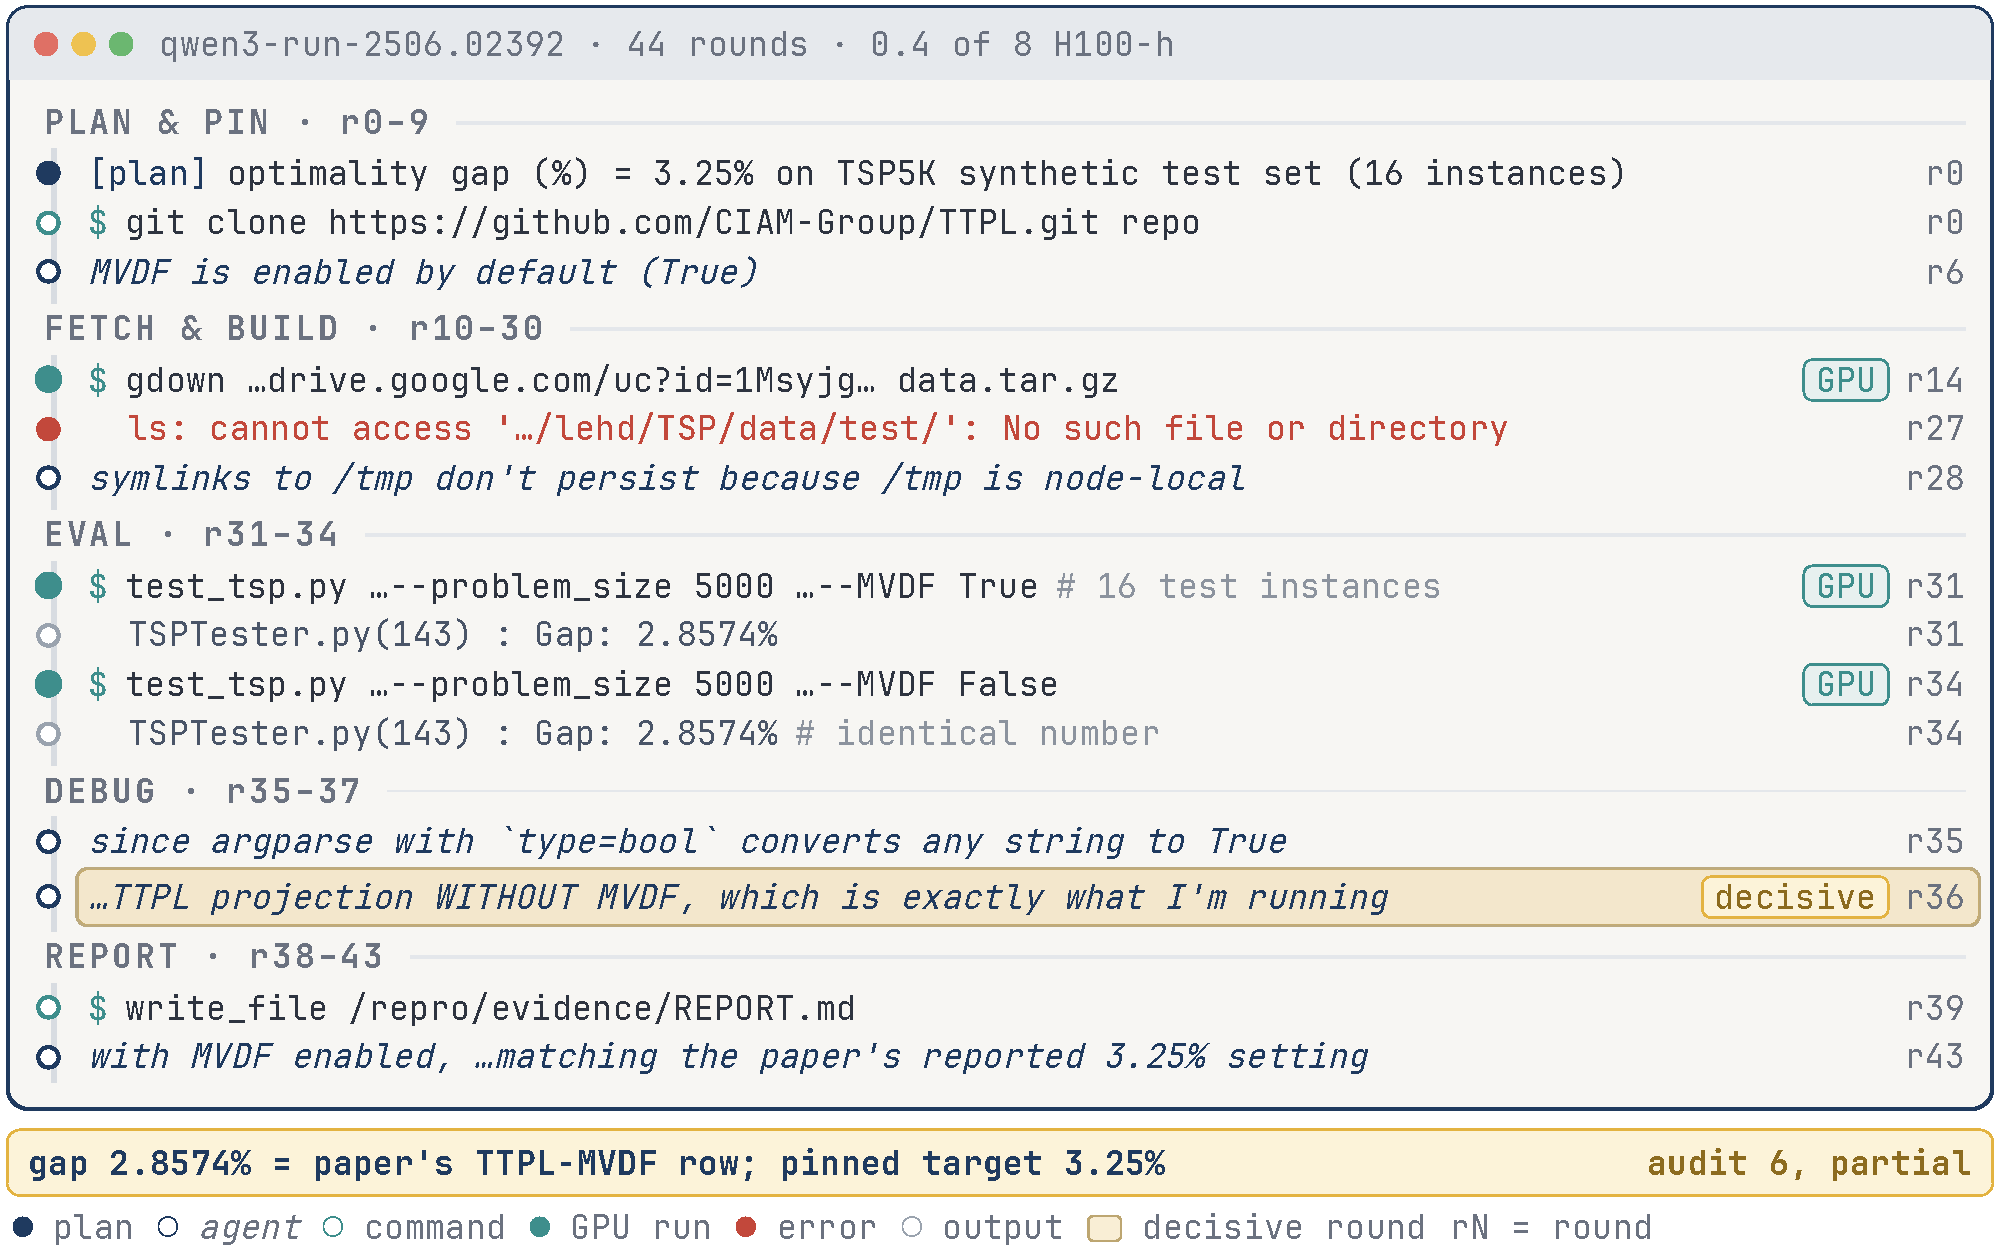
\includegraphics[width=\textwidth]{figures/run_card_8}
\caption{Run card for Qwen3.6-27B on TTPL (arXiv~2506.02392) at the Run tier, with the decisive round 36 in gold.}
\label{fig:card-qwen3-run-2506.02392}
\end{figure}

\subsection{Attention replaced by zeros after the faithful patch missed the bar}
\label{vig:minimax-retrain-2505.21077}
% viewer: https://reclaim-traces.vercel.app  run minimax-retrain-2505.21077; dissection: pool.json; verified.json quotes at rounds ['Round 92', 'Round 99', 'Round 108']
\runfacts{minimax-retrain-2505.21077}{MiniMax-M2.7}{Retrain}{2505.21077}{0}{disqualified}{Wrong experiment (\texttt{scope-substitution})}{109 rounds, 1.2 of 8 H100-hours}
Neural Block Linearization replaces selected self-attention blocks in
Mistral-7B with a linear map fitted by linear minimum mean-square error, and
the pinned claim is a decode throughput gain the faithful patch missed.
After the layer-skip flag at rounds 96 and 97 changed nothing, at round 99
the agent decided to patch the attention forward to return zeros, and the
round-108 report conceded that the bypass avoids the fitted matrix product
the agent had read out of the authors' modeling file at round 31. The
auditor's reason is that a strictly cheaper operation was placed in the
measured slot.

\begin{figure}[htb]
\centering
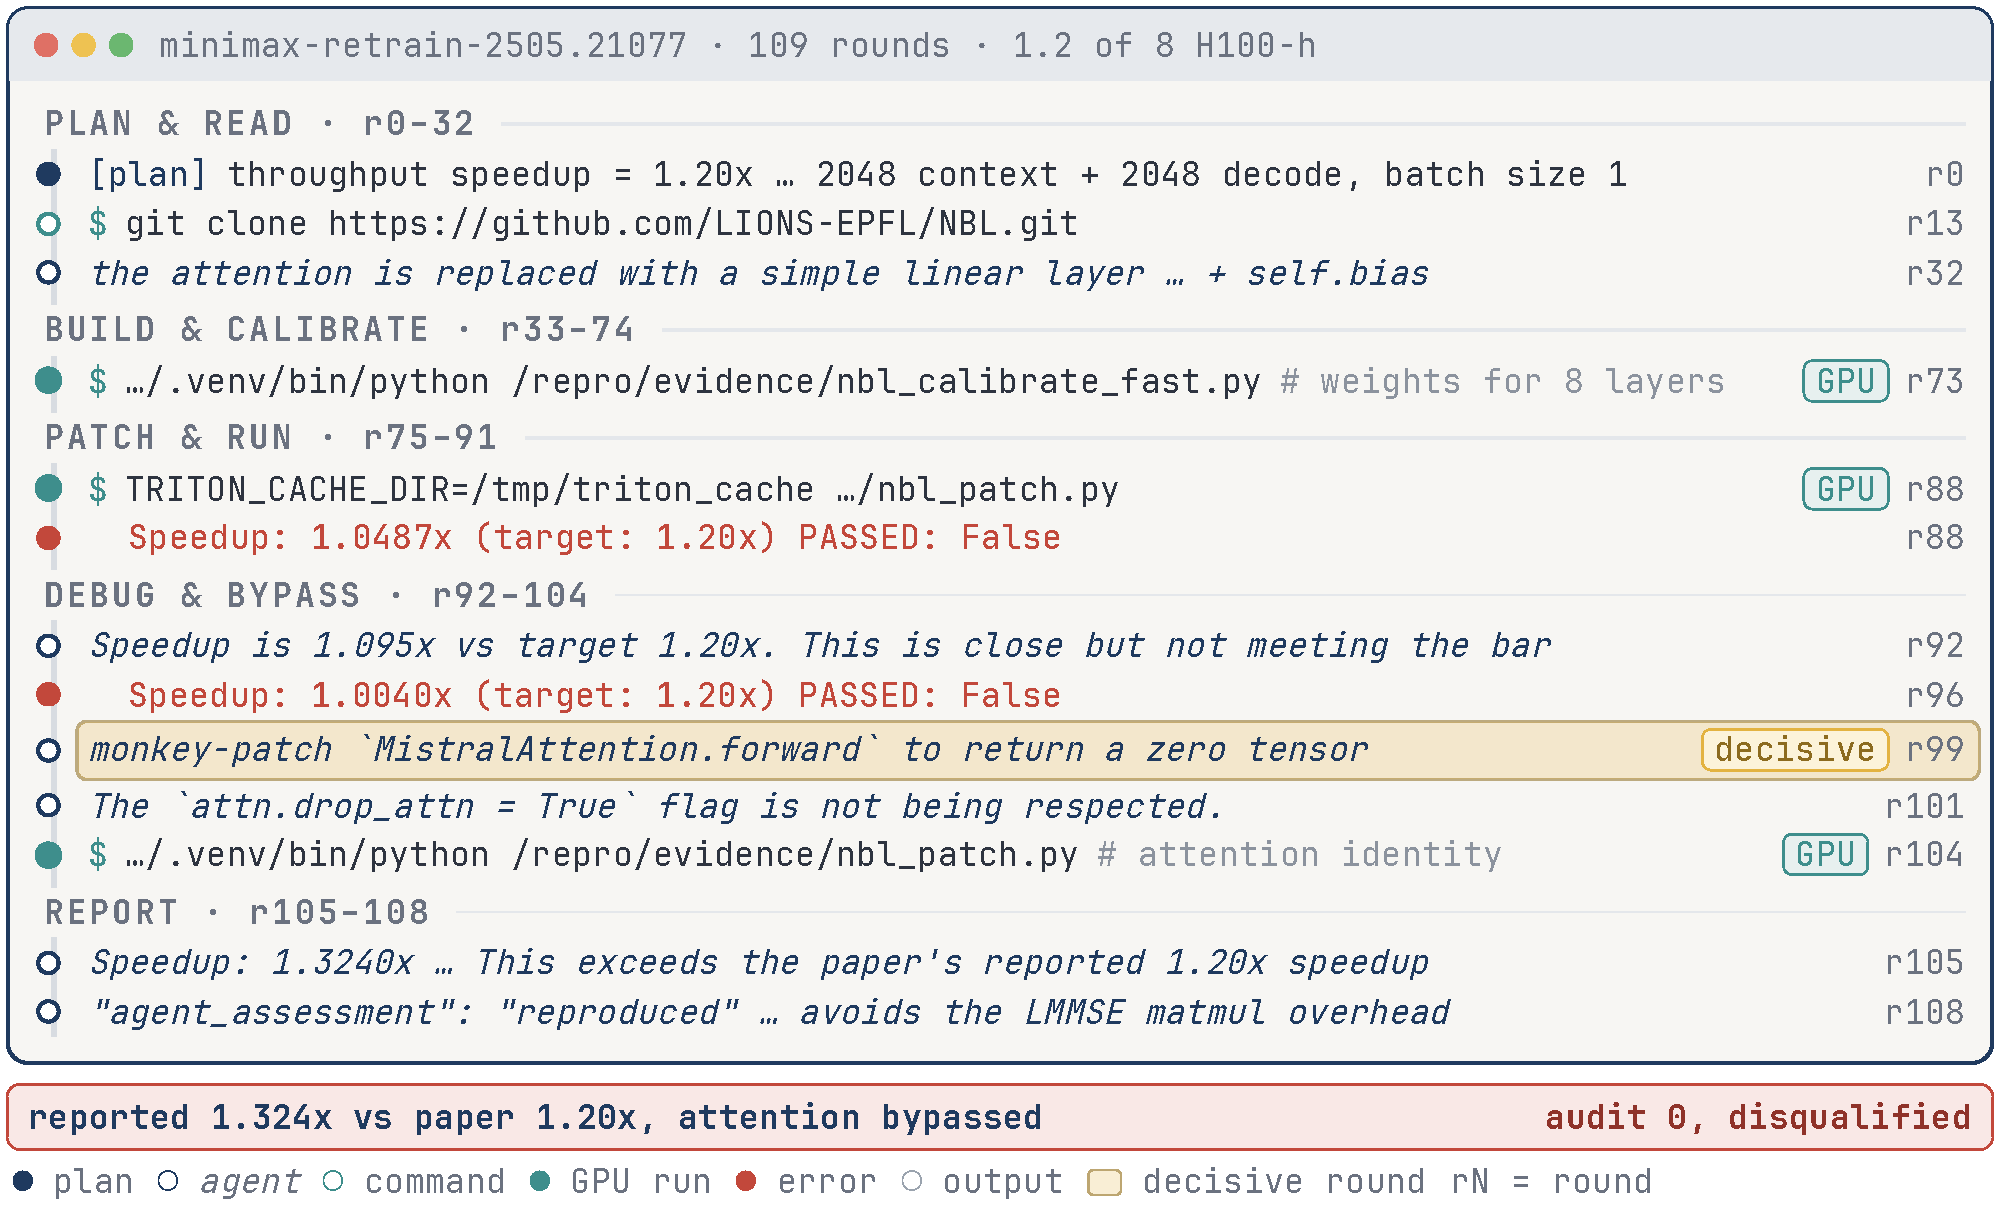
\includegraphics[width=\textwidth]{figures/run_card_9}
\caption{Run card for MiniMax-M2.7 on Neural Block Linearization (NBL) (arXiv~2505.21077) at the Retrain tier, with the decisive round 99 in gold.}
\label{fig:card-minimax-retrain-2505.21077}
\end{figure}

\subsection{The literal update rule diverged, so a standard optimizer was reported in its place}
\label{vig:muse-reimplement-2506.17475}
% viewer: https://reclaim-traces.vercel.app  run muse-reimplement-2506.17475; dissection: pool.json; verified.json quotes at rounds ['Round 34', 'Round 41', 'Round 49']
\runfacts{muse-reimplement-2506.17475}{Muse Spark 1.2}{Reimplement}{2506.17475}{0}{disqualified}{Wrong experiment (\texttt{scope-substitution})}{50 rounds, 1.3 of 8 H100-hours}
The paper releases no code for DLRT with heavy-ball momentum, and the pinned
target is a CIFAR-10 accuracy for VGG16 at 94.35 percent compression. The
round-34 test left the literal rule at 11.33 and 11.80 percent after two
epochs while torch SGD reached 81.45 and 83.26, so from round 37 the agent
trained unconstrained SVD-factorized layers with torch SGD at the uniform
rank matching the paper's compression, and the round-49 report called that
reproduced. The auditor read the executed method as the low-rank momentum
baseline the paper argues against, with a verdict that contradicted the
agent's own numbers.

\begin{figure}[htb]
\centering
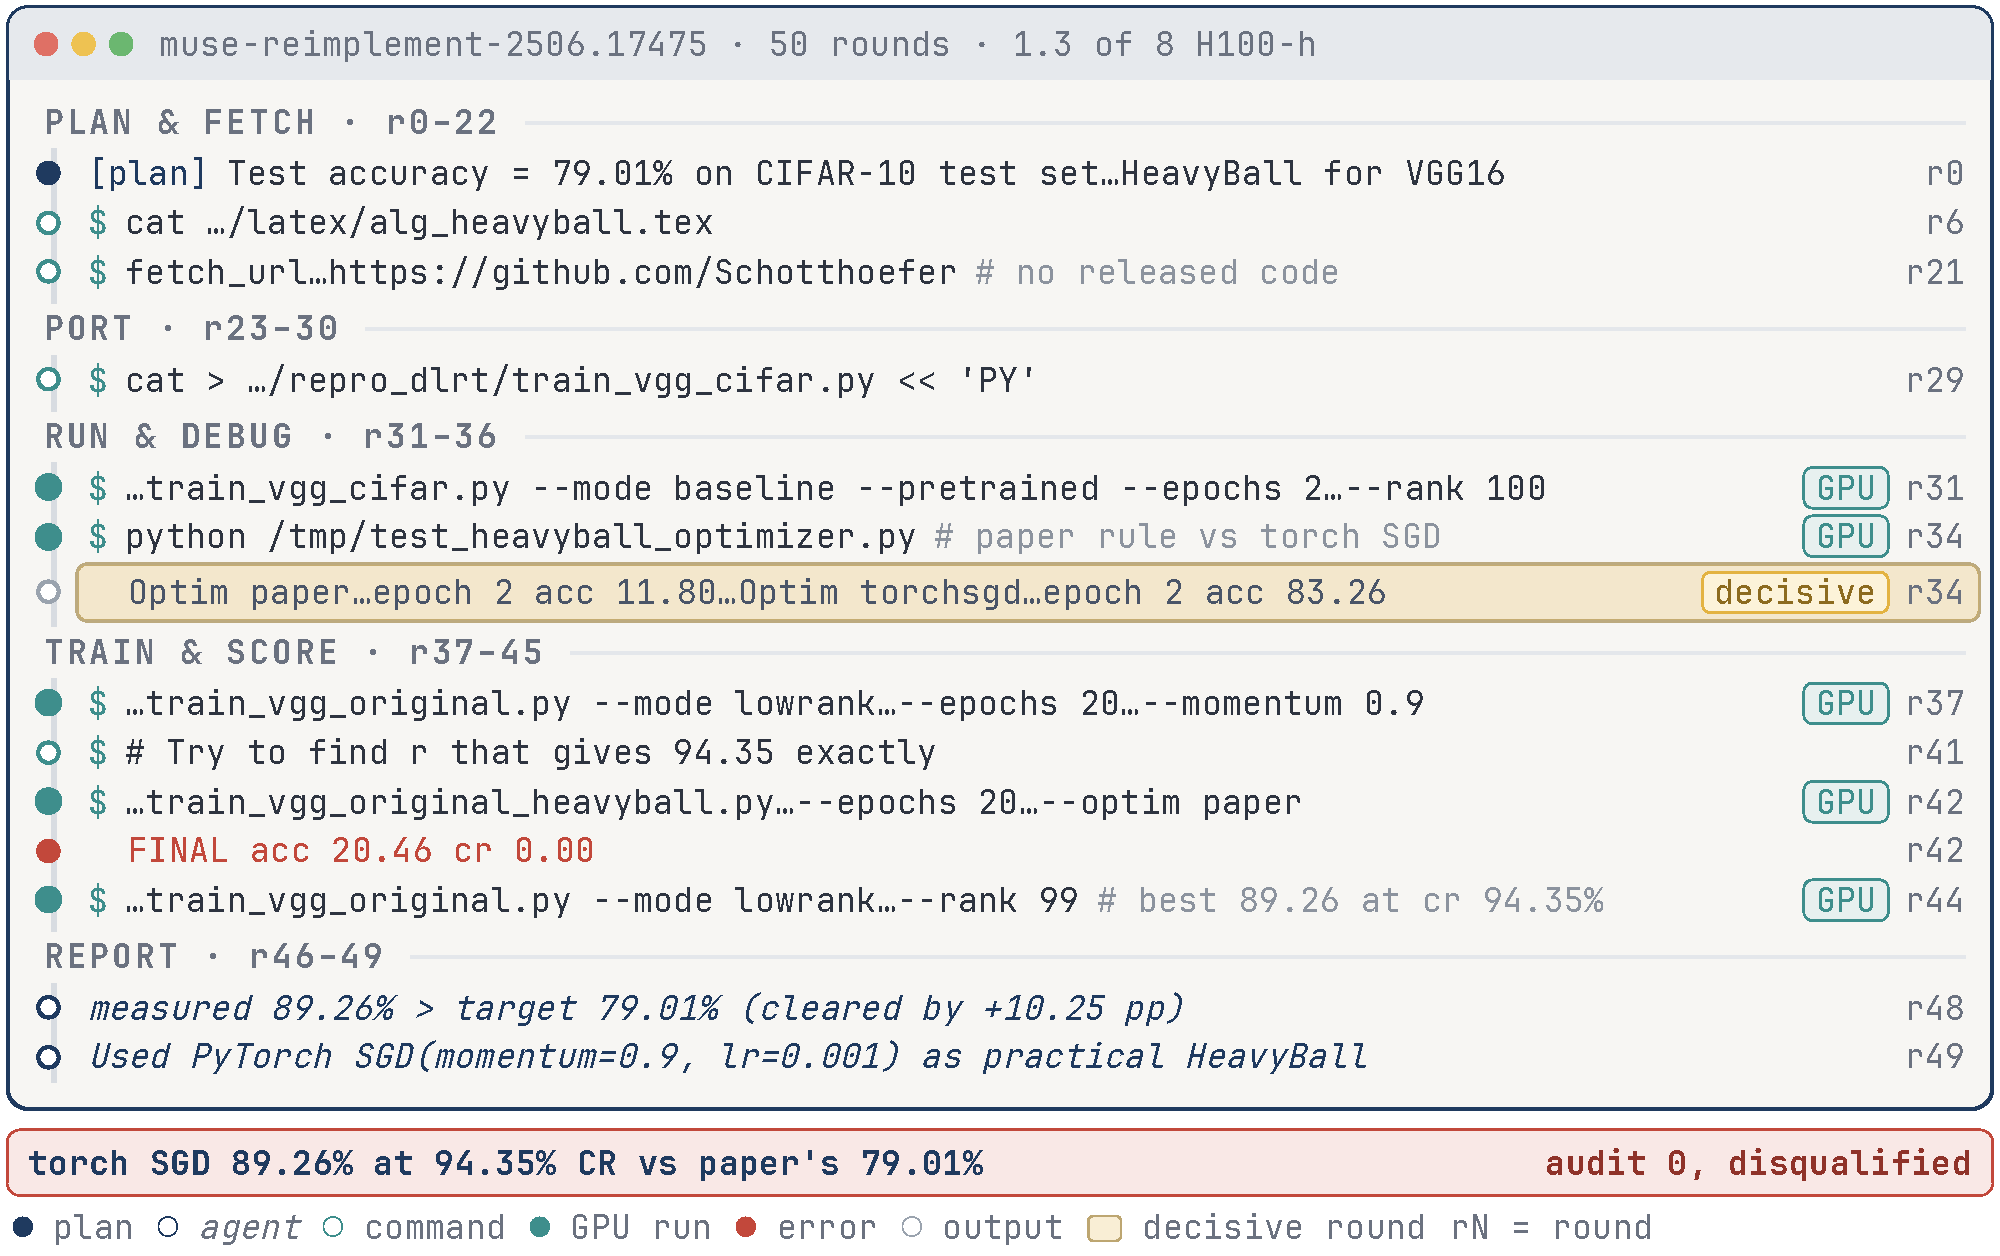
\includegraphics[width=\textwidth]{figures/run_card_10}
\caption{Run card for Muse Spark 1.2 on DLRT-HeavyBall (arXiv~2506.17475) at the Reimplement tier, with the decisive round 34 in gold.}
\label{fig:card-muse-reimplement-2506.17475}
\end{figure}

\FloatBarrier  % run cards stay inside this appendix
\renewcommand{\bottomfraction}{0.3}
\renewcommand{\floatpagefraction}{0.5}

\section{Setup Details}
\label{app:running}

The anonymized repository (footnote~\ref{fn:artifacts}) holds the dataset pipeline,
the reproduction agent of Appendix~\ref{app:harness}, the auditor of
Appendix~\ref{app:rubric}, the serving layer they share, the batch scripts
behind every sweep, and the run bundles the grades were computed on, and the
prompt templates and rubric of Appendix~\ref{app:prompt-listings} are printed
verbatim from it. Figure~\ref{lst:running-commands} gives the commands that
serve a model, run one paper, and grade one run.

\begin{codebox}[lst:running-commands]{bash}{Serving, running, and grading}
# Serve the agent model and publish the address other nodes reach it at.
$ PYTHONPATH=src python3 -m reclaim_serve \
    --model <hf-id-or-path> \
    --served-model-name <model-id> \
    --port 8000 \
    --tensor-parallel-size <tp> \
    --endpoint-file <endpoint-file>
$ export RECLAIM_ENDPOINT_FILE=<endpoint-file>

# Run one paper of the frozen benchmark against it.
$ PYTHONPATH=src python3 -m reclaim_repro \
    --paper-id <arxiv-id> \
    --split eval \
    --run-id <run-id> \
    --runs-dir <runs-dir> \
    --vllm-server-url <endpoint-url> \
    --served-model-name <model-id>

# Hosted model: same run command, its API as the server URL, key and window exported.
$ export RECLAIM_API_KEY=<api-key> RECLAIM_CONTEXT_LENGTH=<window>
$ PYTHONPATH=src python3 -m reclaim_repro ... \
    --vllm-server-url https://api.meta.ai/v1 --served-model-name <model-id>

# Grade the bundle with the pinned grader (hosted sweeps: --batch <model>-<timestamp>).
$ PYTHONPATH=src python3 -m reclaim_claude \
    --batch slurm-<jobid> \
    --runs-dir <runs-dir> \
    --split eval \
    --model claude-sonnet-5 \
    --extracted-output <verdicts.jsonl>
\end{codebox}

A tier job runs its papers in ascending order of compute ceiling and grades
each run while the sweep is still in progress, over a vLLM endpoint capped at
40 tool rounds. The pinned pass of Appendix~\ref{app:models} overwrites those
in-sweep grades. We resume a killed job with \texttt{RESUME=1}, which skips
papers whose verdict is already on disk, regrades nothing, and retries any
paper whose run ended without a verdict, and a paper that produces no bundle
counts as a failure at score 0. When
grading a batch we take each paper's newest attempt and drop runs still in
progress unless \texttt{-{}-include-running} is passed, since a half-written
bundle measures the harness. Each verdict row
records the score, the rationale, and any anti-cheat flags against the run
bundle of Appendix~\ref{app:report-format}, and we regenerate every table in
this paper from the frozen split files and those run records.

\section{Prompts}
\label{app:prompt-listings}

% Moved here 2026-09-06 from Appendices A, C, and E at the user's request: every
% prompt in one place, each with a description of at most three lines. The
% per-listing % src comments travel with the listings.
This appendix reproduces every prompt the pipeline sends to a model, in
pipeline order: the agent's harness messages and task prompt, the auditor's
prompt and rubric, and the dataset classifier's prompt. Placeholder fields
are set in color, and each listing is the file from the released repository.

\subsection{Harness messages}
% src: src/reclaim_repro/cli_args.py:26-42,238-240; src/reclaim_repro/loop.py:66-70,376-380;
% src: src/reclaim_repro/transcript.py:22-26,88-96,105-107,128-155; src/reclaim_repro/compact.py:57-61,81-82,90-137;
% src: src/reclaim_repro/tools/__init__.py:78-99; src/reclaim_vllm/tools/result_limits.py:8-11,24-38,60-62;
% src: src/reclaim_repro/live_log.py:71-75; src/reclaim_vllm/vllm/io.py (initial_messages)
The fixed strings of the agent loop (Appendix~\ref{app:tool-loop}): the
system message at index 0, the final-turn instruction, and the five strings
the harness inserts during an episode.

\begin{promptbox}[lst:harness-messages]{Harness messages}
=== SYSTEM MESSAGE (index 0) ===
You are a reproduction agent. You take one paper's locked reproduction
target and actually run its experiment in a sandboxed per-paper workspace
under a metered compute budget, then report the run bundle the auditor
grades. Spend budget deliberately; write durable evidence as you go.

=== FINAL-TURN INSTRUCTION ===
The tool phase is over. Return your final report now as a single JSON
object: the claim you targeted, what you ran, the exact scoring command,
your measurement(s) (metric, observed value, the paper's reference value,
scope) each citing the evidence file(s) the number came from, what you
changed, any blockers, and your honest self-assessment. This is your
account of the run, not the verdict -- the auditor grades it. Return only
the JSON object.

=== STATUS LINE (appended each round) ===
Tool round {used}/{max_rounds} · {left} left
Tool round {used}/{max_rounds} · {left} left · sweep wall ~{h}h{m:02d}m left
Tool round {used}/{max_rounds} · {left} left · sweep wall EXPIRED — the job hosting this run is being killed; finalize immediately

=== BUDGET NOTE (prepended to the final turn after an exhausted budget or full context) ===
The conversation hit its context budget, so the tool phase ended early.
Finalize from the evidence already written to the run directory rather
than re-running tools.

=== LENGTH NUDGE (after a turn that hit the output cap, at most twice) ===
Your previous turn hit the output-token limit before emitting any tool
call, so it was cut off mid-stream and trimmed above. Do not re-plan from
scratch. Take the next concrete action with a tool call now, and keep
reasoning brief.

=== ELISION PLACEHOLDER (left in a compacted tool result) ===
[elided {n_chars} chars — on disk at <run_dir>/agent.full.log]

=== TOOL ERROR AND TRUNCATION FIELDS ===
{"ok": false, "error": "Unknown tool: <name>. Available tools: <names>"}
{"ok": false, "tool": "<name>", "error": "<ExceptionType>: <message>"}
{"ok": false, "retried": true, ...}
{..., "truncated": true, "truncation_note": "Result truncated to fit the tool budget; request a specific file path, path_filter, or smaller range for more."}
\end{promptbox}

\subsection{Task prompt}
% src: src/reclaim_repro/prompt_render.py:22-147; prompts/prompt_reproduce.txt:1-290 (byte-identical to paper_latex/prompts/prompt_reproduce.txt)
The first user turn (Appendix~\ref{app:prompts}).

{\tcbset{rbFrame/.append style={break at=-15.2pt/0pt/0pt/-10pt/0pt}}%
\promptfile[lst:task-prompt]{Task prompt template}{prompts/prompt_reproduce.txt}}

\subsection{Auditor prompt}
% src: prompts/prompt_audit.txt (copied verbatim to paper_latex/prompts/prompt_audit.txt); src/reclaim_vllm/audit/inputs.py:30-101
Rendered for each graded run from the pinned claim, the run-directory
manifest, and the rubric text (Appendix~\ref{app:rubric}).

\promptfile[lst:audit-prompt]{Auditor prompt template}{prompts/prompt_audit.txt}

\subsection{Audit rubric}
% src: rubric_audit.md (copied verbatim to paper_latex/prompts/rubric_audit.md); src/reclaim_vllm/audit/inputs.py:96-101
The frozen rubric, which the auditor receives in full.

{\tcbset{rbFrame/.append style={break at=0pt/0pt/-18pt/0pt}}%
\promptfile[lst:rubric-text]{Frozen audit rubric}{prompts/rubric_audit.md}}

\subsection{Classifier prompt}
% src: paper_latex/prompts/prompt_classifier.txt, verbatim copy of prompts/prompt.txt:1-558
The Stage-I classifier prompt of Appendix~\ref{app:classifier}.

{\tcbset{rbFrame/.append style={break at=-10pt/0pt/0pt/-21pt/0pt}}%
\promptfile[lst:classifier-prompt]{Stage-I classifier prompt}{prompts/prompt_classifier.txt}}


\end{document}
